\chapter{Zeta jets, Stieltjes antiderivatives and negative polygamma}
\label{ch:07-integration}

The gamma function is the first spectral derivative of Hurwitz zeta at zero.
Further derivatives give a natural language for integrating Stieltjes
functions. Integration in the Hurwitz parameter moves the spectral argument
downward, creating the negative-order polygamma ladder. This chapter develops
that common mechanism before tabulating its moments and rational values.

\section{Below the digamma: \texorpdfstring{$\psi^{(-2)}$}{psi(-2)} at rationals}
\label{integral:sec:psim2}

One integration below the digamma sits $\psi^{(-2)}(z)=\int_0^z\log\Gamma(t)\,dt$.
At denominators $3,4,6$, reflection and distribution reduce the
integral to Clausen values, $\zeta'(-1)$ and logarithms. The odd character
part is Clausen-explicit at general rational points, but the even part
can retain Dirichlet derivatives. The three original examples below are
correct; their earlier extrapolation to every denominator was too broad.

\begin{result}[log-gamma integrals in the Clausen lattice]\label{integral:res:loggamma}
\begin{align*}
\int_0^{1/4}\log\Gamma(t)\,dt
&=\frac{3}{32}+\frac{\log2}{8}+\frac{\log\pi}{8}
+\frac{\Catalan}{4\pi}-\frac{9}{8}\,\zeta'(-1),\\[4pt]
\int_0^{1/3}\log\Gamma(t)\,dt
&=\frac{1}{9}+\frac{\log2}{6}-\frac{\log3}{72}+\frac{\log\pi}{6}
+\frac{\Cl_2(2\pi/3)}{4\pi}-\frac{4}{3}\,\zeta'(-1),\\[4pt]
\int_0^{1/6}\log\Gamma(t)\,dt
&=\frac{5}{72}+\frac{7\log2}{72}+\frac{\log3}{144}+\frac{\log\pi}{12}
+\frac{\Cl_2(\pi/3)}{4\pi}-\frac{5}{6}\,\zeta'(-1).
\end{align*}
\end{result}

The structural punchline: the quarter-point integral carries Catalan
($\Cl_2(\pi/2)=\Catalan$) and the third-point integral carries
$\Cl_2(2\pi/3)=\tfrac23\,\Cl_2(\pi/3)$, two-thirds of Gieseking's constant --- the
``level-3 Catalan'' that had surfaced independently in the
repository's Eisenstein-ladder work --- now arriving from a completely different direction.

\begin{negative}[recorded on purpose]\label{integral:neg:psim2}
(i) The half-point probe $\int_0^{1/2}\log\Gamma$ initially found no relation --- because
$\log\Gamma(1/2)=\tfrac12\log\pi$ made the PSLQ basis $\mathbb{Q}$-dependent, and PSLQ
returned that degeneracy instead of the target. Remove known dependencies
or search modulo their known relation space, and require a nonzero target
coefficient. Unknown arithmetic independence is not a prerequisite for
searching or proving a target identity. (ii) A $\psi^{(-3)}(1/4)$ probe via Cauchy's repeated-integration
kernel produced only a large-coefficient candidate (heights $\sim10^6$) with a weak canary
($10^{-46}$ at $100$ dps) --- \emph{rejected} as a PSLQ false positive. The weight-$3$
level needs a properly prepared basis (presumably $\zeta'(-2)$-equivalents plus
Barnes-$G$-layer logarithms).
\end{negative}

\section{The general log-gamma integral and the fifth-point obstruction}
\begin{proposition}[An exact denominator-five correction]
\label{loggamma:corr:loggamma-five}
Let $\chi_5$ be the quadratic character modulo $5$, with values
$(1,-1,-1,1)$ on residues $1,2,3,4$.  Then
\begin{align}
 \int_0^{1/5}\log\Gamma(t)\,dt
 ={}&\frac{2}{25}+\frac{\log(2\pi)}{10}
       +\frac{\operatorname{Cl}_2(2\pi/5)}{4\pi}
       -\frac65\zeta'(-1) \notag\\
    &+\frac1{20}L'(-1,\chi_5)-\frac{29}{1200}\log5.
 \label{loggamma:corr:loggamma-five-formula}
\end{align}
More generally, for $a>0$,
\begin{equation}\label{loggamma:corr:loggamma-general}
 \int_0^a\log\Gamma(t)\,dt
 =\zeta'(-1,a)-\zeta'(-1)
       +\frac{a-a^2}{2}+\frac a2\log(2\pi).
\end{equation}
\end{proposition}
\begin{proof}
Differentiate $\partial_a\zeta(s,a)=-s\zeta(s+1,a)$ with respect to
$s$ at $s=-1$.  Lerch's identity and $\zeta(0,a)=\tfrac12-a$ give
\[
 \partial_a\zeta'(-1,a)
 =\zeta'(0,a)-\zeta(0,a)
 =\log\Gamma(a)-\tfrac12\log(2\pi)-\tfrac12+a.
\]
The shift identity for Hurwitz zeta shows that
$\zeta'(-1,a)\to\zeta'(-1)$ as $a\downarrow0$, since the additional
term is $-a\log a$.  Integration proves
\eqref{loggamma:corr:loggamma-general}.  These are classical Hurwitz-zeta
identities \cite{hstruct:DLMF}; the integrated theory is also developed by
Espinosa and Moll \cite{loggamma:EspinosaMoll2002b}.

Put $Z_r=\zeta'(-1,r/5)$ and $Z=\zeta'(-1)$.  The Fourier reflection
formula at this weight is
\begin{equation}\label{loggamma:corr:zeta-minus-one-reflection}
 \zeta'(-1,a)-\zeta'(-1,1-a)
       =\frac{\operatorname{Cl}_2(2\pi a)}{2\pi},
       \qquad 0<a<1.
\end{equation}
For completeness, subtract the two Hurwitz Fourier expansions
\[
 \zeta(1-s,a)-\zeta(1-s,1-a)
 =\frac{4\Gamma(s)}{(2\pi)^s}\sin\frac{\pi s}{2}
       \sum_{m\geq1}\frac{\sin(2\pi ma)}{m^s}
\]
and differentiate at $s=2$.  Absolute local convergence of the
series and its logarithmic derivative justifies the differentiation;
the zero of the sine factor leaves precisely
\eqref{loggamma:corr:zeta-minus-one-reflection}.

Differentiating distribution and the character decomposition at $s=-1$
gives
\begin{align*}
 Z_1+Z_2+Z_3+Z_4&=-\frac45 Z-\frac{\log5}{60},\\
 Z_1-Z_2-Z_3+Z_4
   &=\frac15\bigl(L'(-1,\chi_5)+\log5\,L(-1,\chi_5)\bigr).
\end{align*}
Here $L(-1,\chi_5)=-2/5$, obtained directly from
$\zeta(-1,a)=-B_2(a)/2$.  Combining these equations with
$Z_1-Z_4=\operatorname{Cl}_2(2\pi/5)/(2\pi)$ yields
\[
 Z_1=-\frac15 Z+\frac1{20}L'(-1,\chi_5)
       -\frac{29}{1200}\log5
       +\frac{\operatorname{Cl}_2(2\pi/5)}{4\pi}.
\]
Insert this into \eqref{loggamma:corr:loggamma-general} at $a=1/5$.
\end{proof}

The correction concerns the scope of the available reduction laws.
It does not prove that $L'(-1,\chi_5)$ is transcendental or independent
of the other constants in \eqref{loggamma:corr:loggamma-five-formula}.  A precise
replacement for the earlier assertion is: the odd reflection component
is Clausen-explicit, while the even component requires the appropriate
Dirichlet-$L$ derivatives unless further relations have been proved.
The general Hurwitz-jet ladder below agrees with this corrected scope.
\section{Binet's second formula and Malmsten's integrals: the Lambert-kernel face}
\label{integral:sec:binet}

Binet's second formula
\[
\log\Gamma(z)=\Bigl(z-\tfrac12\Bigr)\log z-z+\tfrac12\log(2\pi)
+2\int_0^\infty\frac{\arctan(t/z)}{e^{2\pi t}-1}\,dt
\]
is the integrated Abel--Plana formula with the \emph{Lambert kernel} $1/(e^{2\pi t}-1)$ ---
the same kernel whose moment sums are the Eisenstein $q$-series of the companion CM
article. Malmsten/Vardi log-log integrals $\int_0^1\ln\ln(1/x)\,R(x)\,dx$ are the
\emph{Mellin avatars} of Kummer's Fourier series: expanding the rational kernel $R$ in a
geometric series produces $L'(\chi,1)$-type sums, and Kummer's formula converts
odd-character $L'(1)$ into $\log\Gamma$ at rationals.

\begin{result}\label{integral:res:binet}
Binet's formula replays exactly at $z=1,\tfrac12,\tfrac14$ \dps{residuals $\le10^{-52}$},
turning every $\Gamma$-store atom into a closed-form arctan--Lambert integral; e.g.
\[
\int_0^\infty\frac{\arctan(4t)}{e^{2\pi t}-1}\,dt
=\frac{1}{2}\Bigl[\log\Gamma\bigl(\tfrac14\bigr)-\tfrac12\log2+\tfrac14
-\tfrac12\log(2\pi)\Bigr].
\]
\end{result}

\begin{result}[Vardi's integral \cite{bridge:Vardi}, re-derived blind]\label{integral:res:vardi}
PSLQ over $\{\pi\gamma,\ \pi\log2,\ \pi\log\pi,\ \pi\log\Gamma(1/4)\}$, with the $\gamma$
atom \emph{declined} (coefficient $0$) \dps{canary exact at $80$ dps}:
\[
\int_0^1\frac{\ln\ln(1/x)}{1+x^2}\,dx=\frac{\pi}{4}\,
\ln\!\Bigl(\frac{4\pi^3}{\Gamma(1/4)^4}\Bigr).
\]
The $q=3$ Malmsten variant \dps{canary $3.4\times10^{-81}$; $\gamma$ declined again}:
\[
\int_0^1\frac{\ln\ln(1/x)}{1+x+x^2}\,dx
=\frac{\pi}{6\sqrt3}\,\ln\!\Bigl(\frac{2^8\pi^8}{3^3\,\Gamma(1/3)^{12}}\Bigr).
\]
\end{result}

Both integrals carry exactly the harvested-$\Gamma$-store atoms: the log-log family is a
systematic \emph{integral-representation generator} for the identity stores --- every odd
Dirichlet character (each denominator $q$) yields one such evaluation through Kummer's
formula, with the $\Gamma$-lattice reducer supplying the closed form mechanically.

\section{The log-gamma moment ladder}\label{integral:sec:moments}

\begin{result}[Hurwitz ladder; classical (Whittaker--Watson \cite{bridge:WhittakerWatson})]\label{integral:res:hurwitzladder}
For $\Real z>0$, use the holomorphic branch of $\log\Gamma(z)$
that is real on the positive axis, and the principal logarithm of $z$. Then
\[
\log\Gamma(z)=\Bigl(z-\tfrac12\Bigr)\log z-z+\tfrac12\log(2\pi)
+\frac12\sum_{n\ge2}\frac{n-1}{n(n+1)}\,\zeta(n,z+1)
.
\]
The series is absolutely and locally uniformly convergent in this
half-plane. On $\Real z\ge\sigma>0$, its Hurwitz terms are bounded
by $\zeta(n,1+\sigma)$, a geometrically decaying majorant. The domain
matters: at $z=-1/2$, $\zeta(n,z+1)=(2^n-1)\zeta(n)$ and the
series terms do not tend to zero.
Since $\zeta(n,z+1)$ is $\psi^{(n-1)}(z+1)$ up to factorials, this is a
$\mathbb{Q}$-linear ladder between $\log\Gamma$ and the \emph{entire polygamma tower at
the same point} --- a candidate certificate law binding the $\Gamma$ and trigamma stores
into one linear system.
\end{result}

\begin{result}[second moment; classical (Espinosa--Moll \cite{bridge:EspinosaMoll})]\label{integral:res:em}
With $L=\log(2\pi)$,
\[
\int_0^1\bigl[\log\Gamma(x)\bigr]^2dx
=\frac{\gamma^2}{12}+\frac{\pi^2}{48}+\frac{\gamma L}{6}+\frac{L^2}{3}
-(\gamma+L)\frac{\zeta'(2)}{\pi^2}+\frac{\zeta''(2)}{2\pi^2}
.
\]
The quadratic-moment layer adds $\zeta''(2)$ to the atom inventory.
\end{result}

The numerical cubic moment originally suggested enlarging the constant
basket. Its known Tornheim representation and the convergent certificate
below settle that representation question; reduction to a specified smaller
algebra remains separate.\label{integral:neg:cubic}

% Analytic research contribution.  The parent article supplies theorem environments.
% Compiled mathematics and provenance: manuscript commit afed07429d3d37eceb6c8e9e54cf4da2d3f39d53.
\section{Log-gamma moments: poles, late coefficients, and effective remainders}
\label{gaussian:sec:gamma}
Let
\[
 M_n=\int_0^1\log^n\Gamma(x)\,dx,\qquad L=\log(2\pi),\qquad A=\gamma+L.
\]
The cubic moment is a test of whether an experiment has selected the right
coordinate system. Bailey, D.~Borwein and J.~M.~Borwein evaluated it in
Tornheim derivatives~\cite[Theorem~6]{gaussian:BBB}. A smaller single-zeta
basket can miss that structure; failure of such a search gives no independence
theorem. We give the explicit representation and its convergence proof.

Similarly, the full fixed-order expansion of $M_n/n!$ into the exponential
scales $k^{-n}$ is Theorem~8.1 of Amdeberhan et al.\ \cite{gaussian:ACEMKM}.
The results proved below add an explicit late-coefficient asymptotic, identify
the divergent character of that expansion, and give a uniform remainder
bound when the number of retained terms grows linearly with $n$.
These are refinements of a known expansion, not a claim to have discovered
that expansion or the cubic Tornheim representation.

\subsection{A compact form of the cubic identity}
Define the holomorphic germ near $(1,1,1)$
\[
 T(r,s,t)=\sum_{m,n\ge1}\frac{1}{m^r n^s(m+n)^t}.
\]
A subscript $j$ denotes partial differentiation in its $j$th argument;
all unmarked Tornheim terms in the next formula are evaluated at $(1,1,1)$.
The double sums and all the derivatives used here converge absolutely.

\begin{theorem}[Cubic moment in one Tornheim differential operator]
\label{gaussian:thm:cubic-compact}
With $A=\gamma+L$,
\begin{align}
 M_3={}&\frac{L^3}{8}+\frac{\pi^2L}{32}+\frac{3\zeta(3)}{16}
 +\frac{3L}{4\pi^2}
 \bigl(A^2\zeta(2)-2A\zeta'(2)+\zeta''(2)\bigr)\notag\\
 &+\frac{3}{8\pi^2}
 \left(A^2T-2AT_3+2T_{13}-T_{12}\right).
 \label{gaussian:eq:cubic-compact}
\end{align}
This is an equivalent form of the known cubic evaluation in
\cite[Theorem~6]{gaussian:BBB}.
\end{theorem}

\begin{proof}
Write the Kummer Fourier series as
\[
 \log\Gamma(x)=\frac L2+\frac12 C(x)+\frac1\pi S(x),
 \quad C(x)=\sum_{j\ge1}\frac{\cos(2\pi jx)}j,
 \quad S(x)=\sum_{j\ge1}\frac{A+\log j}{j}\sin(2\pi jx).
\]
Reflection $x\mapsto1-x$ makes $C$ even and $S$ odd.  Parseval gives
\[
 \int_0^1 C^2=\frac12\zeta(2),\qquad
 \int_0^1 S^2=\frac12\bigl(A^2\zeta(2)-2A\zeta'(2)+\zeta''(2)\bigr).
\]
The cosine resonance gives $\int C^3=3\zeta(3)/2$.  Equivalently, one can
differentiate the beta integral for $\int_0^1(2\sin\pi x)^u dx$ three times
at zero and use $C=-\log(2\sin\pi x)$.
For the only remaining cubic term, the elementary product rule for two sines
and one cosine gives
\begin{align*}
 \int_0^1 CS^2
 &=\frac12\sum_{m,n\ge1}
   \frac{(A+\log m)(A+\log(m+n))}{mn(m+n)}\\
 &\hspace{1em}-\frac14\sum_{m,n\ge1}
   \frac{(A+\log m)(A+\log n)}{mn(m+n)}\\
 &=\frac14\left(A^2T-2AT_3+2T_{13}-T_{12}\right).
\end{align*}
Expansion of the cube now proves the formula.

For the convergence justification, first put an Abel factor $r^j$ in every
Fourier series, $0<r<1$.  All products can then be integrated termwise.
The functions $C$ and $S$ belong to every finite $L^p(0,1)$, since the
identities with $\log\Gamma(x)$ and $\log\Gamma(1-x)$ bound them by
endpoint logarithms.  Poisson convolution therefore converges to them in
$L^3$, so the integrated cubic products converge.  In the resulting
resonance sums the logarithmic numerator is bounded by a constant times
$(1+\log(m+n))^2$.  Summing first over $m+n=q$ uses
\[
 \sum_{m=1}^{q-1}\frac{1}{m(q-m)q}=\frac{2H_{q-1}}{q^2},
\]
which proves absolute convergence and legitimizes the Abel limit.
\end{proof}

The double-coordinate derivative in \eqref{gaussian:eq:cubic-compact} can also be
written as a positive sum.  Put
\[
 \mathcal R_A=\sum_{m,n\ge1}
 \frac{(A+\log(m+n))^2-
 \log((m+n)/m)\log((m+n)/n)}{mn(m+n)}.
\]
Symmetry in $m,n$ proves
$\mathcal R_A=A^2T-2AT_3+2T_{13}-T_{12}$.
The numerator is positive: after expansion it is
$A^2+2A\log(m+n)+(\log m+\log n)\log(m+n)-\log m\log n$.
It is bounded above by $(A+\log(m+n))^2$.
Consequently, if $\mathcal R_{A,N}$ restricts $m+n\le N$ and $N\ge3$ is an integer, then
\begin{equation}
 0<\mathcal R_A-\mathcal R_{A,N}
 \le\frac2N\bigl(P(\log N)+P'(\log N)+P''(\log N)+P'''(\log N)\bigr),
 \quad P(u)=(1+u)(A+u)^2.
 \label{gaussian:eq:tornheim-tail}
\end{equation}
Indeed $H_{q-1}\le1+\log q$, and
$(1+\log x)(A+\log x)^2/x^2$ decreases for $x\ge3$.
Integration of the resulting tail gives \eqref{gaussian:eq:tornheim-tail}.
This bound is elementary and rigorous but converges only as
$O(\log^3N/N)$; it is useful as an independent sign and normalization check,
not as the preferred high-precision algorithm.

\subsection{A positive summand form and an explicit tail bound}

The combination in \eqref{gaussian:eq:cubic-compact} can be computed without cancellation
between separate Tornheim constants.  For $k=m+n$, define
\[
 R_A(m,n)=A^2+2A\log k+\log m\log k+\log n\log k-\log m\log n.
\]
Since $A>0$, $\log k\ge\log m,\log n\ge0$, we have $R_A(m,n)>0$.
Writing $p=\log m,q=\log n,r=\log k$, one also has
$r(p+q)-pq\le r^2$: for fixed $r$, the expression is increasing separately
in $p,q\in[0,r]$.  Consequently
\[
 0<R_A(m,n)\le(A+\log k)^2.
\]
Therefore the diagonal partial sums
\[
 C_N=\frac3{32}\sum_{m+n\le N}\frac1{mn(m+n)}
    +\frac{3}{8\pi^2}
       \sum_{m+n\le N}\frac{R_A(m,n)}{mn(m+n)}
\]
increase to the centered cubic moment $M_3-a^3-3aV$.  Moreover,
\begin{align*}
 0<(M_3-a^3-3aV)-C_N
 &\le\sum_{k>N}\frac{2(1+\log k)}{k^2}
       \left(\frac3{32}+\frac{3(A+\log k)^2}{8\pi^2}\right).
\end{align*}
This gives a transparent computable enclosure, although its convergence
is only $O(\log^3N/N)$.  An integral bound may be used once the explicit
summand is decreasing; direct summation can handle the finite initial range.
This positivity observation is an immediate corollary of the Fourier
calculation, not a claim of a new classical-constant evaluation.

\subsection{Exponentially convergent numerical reproduction}

For $t>0$, put
\[
 C(t)=\operatorname{Li}_1(e^{-t})=-\log(1-e^{-t}),\qquad
 F(t)=\left.\partial_s\operatorname{Li}_s(e^{-t})\right|_{s=1}.
\]
The usual Mellin representation of the Tornheim sum gives
\begin{equation}\label{tornheim:cubic:mellinpartials}
 T_{12}=\int_0^\infty F(t)^2\,dt,\quad
 T_{13}=\int_0^\infty F(t)C(t)(\log t+\gamma)\,dt,\quad
 T_3=\int_0^\infty C(t)^2(\log t+\gamma)\,dt.
\end{equation}
For $0<t<2\pi$, cancellation of the two poles in Jonqui\`ere's expansion
produces
\begin{align*}
 C(t)&=-\log t+\sum_{k\ge1}c_kt^k,
 &c_k&=\frac{(-1)^k\zeta(1-k)}{k!},\\
 F(t)&=-\alpha-\gamma\log t-\tfrac12\log^2t+\sum_{k\ge1}b_kt^k,
 &b_k&=\frac{(-1)^k\zeta'(1-k)}{k!},\\
 \alpha&=\gamma_1+\frac{\gamma^2}2+\frac{\pi^2}{12}.
\end{align*}
Here the Stieltjes convention is
$\zeta(1+z)=z^{-1}+\sum_{j\ge0}(-1)^j\gamma_jz^j/j!$.
For computational stability the coefficient formulas can be rewritten as
\begin{align*}
 c_1&=\tfrac12,&b_1&=\tfrac12\log(2\pi),\\
 c_{2j}&=\frac{(-1)^j\zeta(2j)}{j(2\pi)^{2j}},&
 b_{2j}&=c_{2j}\left(\log(2\pi)-\psi(2j)-\frac{\zeta'(2j)}{\zeta(2j)}\right),\\
 c_{2j+1}&=0\quad(j\ge1),&
 b_{2j+1}&=\frac{(-1)^{j+1}\pi\zeta(2j+1)}{(2j+1)(2\pi)^{2j+1}}
 \quad(j\ge1).
\end{align*}
The functional equation of the Riemann zeta function proves these identities.
Elementary bounds $\zeta(k)<2$, $|\zeta'(k)|<2$, $H_{k-1}\le k-1$,
$\gamma<1$, $\log(2\pi)<2$, and $2\pi>6$ give, for $k\ge2$,
\[
 |b_k|\le12\,6^{-k},\qquad |c_k|\le2\,6^{-k}.
\]
Thus after degree $K\ge1$ their remainders on $0<t\le1$ are at most
\[
 \epsilon_b=\frac{12}{5}6^{-K},\qquad
 \epsilon_c=\frac25 6^{-K}.
\]
All integrals of the resulting polynomials in $t$ and $\log t$ are evaluated
using $\int_0^1t^k\log^jt\,dt=(-1)^jj!/(k+1)^{j+1}$.

On $t\ge1$, insert
$C(t)=\sum_{n\ge1}e^{-nt}/n$ and
$F(t)=-\sum_{n\ge1}(\log n)e^{-nt}/n$.  The integral with the logarithmic
factor uses
\[
 \int_1^\infty e^{-kt}(\log t+\gamma)\,dt
 =\frac{E_1(k)+\gamma e^{-k}}k.
\]
Truncate this sum at $m+n\le N$.  A common upper bound for the three
omitted tails is
\[
 B_N=4\sum_{k>N}ke^{-k}
 =\frac{4e^{-(N+1)}((N+1)-Ne^{-1})}{(1-e^{-1})^2}.
\]
For the three integrals in the order $T_{12},T_{13},T_3$, safe total
series-truncation bounds are respectively
\[
 \epsilon_b(12+\epsilon_b)+B_N,\qquad
 5\epsilon_b+15\epsilon_c+2\epsilon_b\epsilon_c+B_N,\qquad
 10\epsilon_c+2\epsilon_c^2+B_N.
\]
For example the elementary estimates
$C(t)\le-\log t+1$ and
$|F(t)|\le4-\log t+\tfrac12\log^2t$ on $(0,1]$ imply all the constants
above.  The sharper bound $\int_0^1|F(t)|dt<6$ follows directly from its
coefficient expansion (one may use $0<\alpha<2$).
An elementary verification of the latter constant bound is available:
the defining limit for $\gamma_1$ and the total variation of
$x\mapsto\log x/x$ on $[1,\infty)$ give $|\gamma_1|\le2/e<3/4$;
combine this with $0<\gamma<3/5$ and $3<\pi<\sqrt{12}$.
This is an analytic truncation certificate; floating-point rounding must
be handled separately to turn an implementation into interval arithmetic.

The independent implementation \texttt{verify\_tornheim.py} evaluates the
three partials and compares \eqref{gaussian:eq:cubic-compact} against direct log-gamma
quadrature.  Its output explicitly labels the rounding qualification.

\subsection{A sign check for an auxiliary identity}

If the June 2012 preprint is used, an auxiliary sign should be checked
before copying its Remark~3.  Put
\[
 S_\gamma=\sum_{m,n\ge1}
        \frac{(\gamma+\log m)(\gamma+\log n)}{mn(m+n)}.
\]
Directly expanding the numerator, with absolutely convergent sums, gives
\[
 T_{12}=S_\gamma+2\gamma\bigl(\zeta'(2,1)+\zeta'(3)\bigr)
                  -2\gamma^2\zeta(3).
\]
The coefficient of $S_\gamma$ is positive.  The displayed minus sign in
equations~(63) and~(65) of the author-hosted June 2012 preprint would make
their right side negative, although $T_{12}>0$.  This issue does not
affect the cubic formula proved above.  This note does not assert that
the same typographical error occurs in the final journal typesetting.



\subsection{Meromorphic moment generating function}
For $\Re z<1$, let
\[
 F(z)=\int_0^1\Gamma(x)^z\,dx
     =\sum_{n\ge0}\frac{M_n}{n!}z^n\quad (|z|<1).
\]
The power uses the real logarithm of $\Gamma(x)>0$.  Introduce the positive
numbers
\begin{equation}
 c_k=\frac1k[u^{k-1}]\Gamma(1-u)^k,\qquad k\ge1.
 \label{gaussian:eq:ck-lagrange}
\end{equation}
Their first values are
\[
 c_1=1,\quad c_2=\gamma,\quad
 c_3=\frac{3\gamma^2+\zeta(2)}2,\quad
 c_4=\frac{8\gamma^3+6\gamma\zeta(2)+\zeta(3)}3.
\]
These agree with the coefficients in \cite[Theorem~8.1]{gaussian:ACEMKM}.

\begin{proposition}[All moment poles and their residues]
\label{gaussian:prop:moment-poles}
The function $F$ extends meromorphically to the whole $z$-plane.  Its only
poles are simple poles at every positive integer, with
\[
 \operatorname*{Res}_{z=k}F(z)=(-1)^k k c_k\ne0.
\]
\end{proposition}
\begin{proof}
Fix $0<a<1$ and expand
\[
 \Gamma(x)^z=x^{-z}\Gamma(1+x)^z
 =x^{-z}\sum_{j=0}^{J-1}b_j(z)x^j+x^{J-z}E_J(x,z).
\]
The $b_j$ are entire functions (in fact polynomials) of $z$, and $E_J$ is
uniformly bounded for $0\le x\le a$ and $z$ in compact subsets of the plane.
Integration from zero to $a$ gives
\[
 \sum_{j=0}^{J-1}\frac{b_j(z)a^{j+1-z}}{j+1-z}
 +\int_0^a x^{J-z}E_J(x,z)\,dx.
\]
The second term is holomorphic for $\Re z<J+1$; the integral from $a$ to
one is entire.  Since $J$ is arbitrary, these formulas give the claimed
continuation.  At $z=k$ the residue is
$-b_{k-1}(k)=(-1)^k[u^{k-1}]\Gamma(1-u)^k$.
Finally
\[
 \log\Gamma(1-u)=\gamma u+\sum_{j\ge2}\frac{\zeta(j)}j u^j
\]
has strictly positive coefficients, so \eqref{gaussian:eq:ck-lagrange} is positive.
\end{proof}

The pole at $k$ contributes $(-1)^{k-1}c_k/k^n$ to the Taylor coefficient
of $F$ at zero.  This explains the exponential scales in the known moment
asymptotics, but an infinite partial-fraction sum cannot be inferred
without controlling the growth of $c_k$.  That growth is decisive.

\subsection{Late coefficients and the inverse reciprocal gamma function}
Set $\phi(u)=\Gamma(1-u)$ and let $\tau$ be the unique point in $(0,1)$
satisfying
\begin{equation}
 -\tau\psi(1-\tau)=1.
 \label{gaussian:eq:critical-tau}
\end{equation}
Equivalently $\psi(-\tau)=0$.  Define
\begin{equation}
 \rho=\frac{\tau}{\Gamma(1-\tau)},\qquad
 \alpha=-\log\rho,\qquad
 v=1+\tau^2\psi'(1-\tau),\qquad
 C=\frac{\tau}{\sqrt{2\pi v}}.
 \label{gaussian:eq:critical-constants}
\end{equation}
Numerically,
\begin{align*}
 \tau&=0.50408300826445540925826930453330249895538518236858\ldots,\\
 \rho&=0.28211580900629804215379660062046372823230190757940\ldots,\\
 \alpha&=1.26543762211086561338203591116547399218544556554213\ldots,\\
 v&=2.27159994608893009911993485126846348661898954658806\ldots,\\
 C&=0.13342776130944528489602057053941782432703493711204\ldots.
\end{align*}
These displayed approximations are numerical evaluations; the theorem uses
the exact definitions \eqref{gaussian:eq:critical-tau}--\eqref{gaussian:eq:critical-constants}.

\begin{theorem}[Late-coefficient asymptotic]
\label{gaussian:thm:late-coefficients}
The coefficients \eqref{gaussian:eq:ck-lagrange} satisfy
\begin{equation}
 c_k=C\rho^{-k}k^{-3/2}\bigl(1+O(k^{-1})\bigr).
 \label{gaussian:eq:ck-asymptotic}
\end{equation}
In fact they have a full expansion in inverse powers of $k$.
The power series $h(w)=\sum_{k\ge1}c_kw^k$ has radius of convergence
$\rho$, converges absolutely on $|w|\le\rho$, and satisfies
\[
 h(w)=w\Gamma(1-h(w)),\qquad h(\rho)=\tau.
\]
For every fixed real $n$, the formal moment series
$\sum_{k\ge1}(-1)^{k-1}c_k/k^n$ diverges, since its terms do not tend to zero.
\end{theorem}

\begin{proof}
Let $D=u\,d/du$.  The function
\[
 \mu(u)=D\log\phi(u)=-u\psi(1-u)
 =\gamma u+\sum_{j\ge2}\zeta(j)u^j
\]
is strictly increasing from zero to infinity on $(0,1)$.  Hence
\eqref{gaussian:eq:critical-tau} has exactly one solution.
Moreover $\phi(u)>1$ there, so $0<\rho<1$ and $\alpha>0$.

Write $\phi(u)=\sum_{j\ge0}a_ju^j$ and introduce an integer-valued random
variable $X$ by
\[
 \Pr(X=j)=\frac{a_j\tau^j}{\phi(\tau)}.
\]
All its probabilities are positive, in particular those at $0$ and $1$;
it has lattice span one.  Analyticity of $\phi$ on $|u|<1$ gives an
exponential moment.  Its mean is $\mu(\tau)=1$ and its variance is
$D^2\log\phi(\tau)=1+\tau^2\psi'(1-\tau)=v>0$.
For independent copies and $S_k=X_1+\cdots+X_k$, coefficient extraction gives
\begin{equation}
 c_k=\frac{\tau\rho^{-k}}k\Pr(S_k=k-1).
 \label{gaussian:eq:coefficient-probability}
\end{equation}
Fourier inversion gives
\[
 \Pr(S_k=k-1)=\frac1{2\pi}\int_{-\pi}^{\pi}
 \left(\frac{\phi(\tau e^{it})}{\phi(\tau)}e^{-it}\right)^k e^{it}\,dt.
\]
For $t\ne0$ modulo $2\pi$, the modulus of the bracket is strictly less
than one, because the distribution has positive mass at $0$ and $1$.
On a small interval around zero its logarithm is
$-vt^2/2+O(t^3)$.  Split off the complement of that interval, whose
contribution is exponentially small, and put $t=y/\sqrt{k}$ in the
remaining integral.  Taylor expansion, dominated by a Gaussian on a
shrinking central interval, gives
\[
 \Pr(S_k=k-1)=\frac1{\sqrt{2\pi vk}}\bigl(1+O(k^{-1})\bigr).
\]
For a fully quantitative split, use $|t|\le k^{-2/5}$, the band
$k^{-2/5}<|t|\le\delta$, and the fixed outer band.  On the middle
band the modulus is at most $e^{-c k^{1/5}}$; on the outer band it is
$O(q^k)$ for some $q<1$.  The nominal $k^{-1/2}$ correction on the
central band is odd and integrates to zero.  Taylor expansion to arbitrary
even order with its analytic remainder gives the full inverse-power expansion.  This elementary saddle argument proves
\eqref{gaussian:eq:ck-asymptotic} and avoids any assumption about unexamined complex
critical values of the reciprocal gamma function.

Lagrange inversion gives the stated functional equation for $h$ near zero.
Equation \eqref{gaussian:eq:ck-asymptotic} proves that its radius is $\rho$ and that
it converges absolutely at the boundary.  On $[0,\tau]$, the function
$f(u)=u/\phi(u)$ increases from zero to $\rho$, with positive derivative
before $\tau$, since $f'(u)=(1-\mu(u))/\phi(u)$.  Its inverse is the
positive real branch of $h$, hence continuity at the boundary gives
$h(\rho)=\tau$.  Finally \eqref{gaussian:eq:ck-asymptotic} proves the stated divergence.
\end{proof}

For completeness, the first correction in \eqref{gaussian:eq:ck-asymptotic} is
\[
 c_k=C\rho^{-k}k^{-3/2}\left(1+\frac{\beta_1}{k}+O(k^{-2})\right),
\]
where, with $\kappa_j=D^j\log\phi(\tau)$,
\begin{align*}
 \beta_1&=-\frac1{2v}+\frac{\kappa_3}{2v^2}
 +\frac{\kappa_4}{8v^2}-\frac{5\kappa_3^2}{24v^3}
 \\
 &=0.30196282878120524112458668271647811378573305248468\ldots.
\end{align*}
This follows by retaining the quartic and squared cubic terms, together
with the factor $e^{it}$, in the Fourier integral.

\subsection{An effective remainder with a growing number of terms}
\begin{theorem}[Explicit truncation bound]
\label{gaussian:thm:effective-moment}
For integers $n\ge1$ and $K\ge1$ with $K\alpha<n$, put
\[
 R_{n,K}=\frac{M_n}{n!}-\sum_{k=1}^{K}\frac{(-1)^{k-1}c_k}{k^n}.
\]
Then, writing $\Gamma(n,z)=\int_z^\infty t^{n-1}e^{-t}\,dt$,
\begin{equation}
 |R_{n,K}|\le
 \frac{\alpha^n}{n!}\left(1+\frac{n\tau}{n-K\alpha}\right)
 +\frac{\tau\rho^{-(K+1)}}{(K+1)^n}
   \frac{\Gamma(n,(K+1)\alpha)}{\Gamma(n)}.
 \label{gaussian:eq:remainder-exact}
\end{equation}
In particular, whenever $n\ge\max\{2,4\alpha^2\}$, the choice
$K=\lfloor n/\alpha-\sqrt n\rfloor$ is positive and gives
\begin{equation}
 |R_{n,K}|\le
 \left(\frac1{\sqrt{2\pi n}}+
       \frac{\tau}{\alpha\sqrt{2\pi}}+
       \tau e^{2\alpha^2}\right)
 \left(\frac{e\alpha}{n}\right)^n.
 \label{gaussian:eq:remainder-optimized}
\end{equation}
\end{theorem}
In particular every integer $n\ge7$ meets the displayed hypothesis.
Indeed $\rho\ge1/(2\sqrt\pi)$ by evaluating $u/\Gamma(1-u)$
at $u=1/2$, and therefore $\alpha\le\log(2\sqrt\pi)<13/10$,
so $4\alpha^2<169/25<7$.

\begin{proof}
The function $\log\Gamma(x)$ decreases strictly from infinity to zero on
$(0,1]$, because $\psi'(x)>0$ and $\psi(1)=-\gamma<0$.
Let $x(y)\in(0,1]$ be its inverse.  The layer-cake formula, or integration
by parts after this monotone change of variables, gives
\begin{equation}
 \frac{M_n}{n!}=\frac1{\Gamma(n)}\int_0^\infty y^{n-1}x(y)\,dy.
 \label{gaussian:eq:moment-inverse}
\end{equation}
For $y\ge\alpha$, Lagrange inversion and continuity on the convergence
circle give
\[
 x(y)=-h(-e^{-y})=\sum_{k\ge1}(-1)^{k-1}c_ke^{-ky}.
\]
The identity initially holds for sufficiently large $y$ and extends along
the negative real inverse branch.  This branch cannot fail before
$w=-\rho$: for $0<x\le1$, the derivative of $1/\Gamma(x)$ is
$-\psi(x)/\Gamma(x)>0$.

For $y\ge\alpha$, positivity and $\sum c_k\rho^k=\tau$ give
\[
 \left|x(y)-\sum_{k=1}^{K}(-1)^{k-1}c_ke^{-ky}\right|
 \le\tau\rho^{-(K+1)}e^{-(K+1)y}.
\]
Integrating this on $[\alpha,\infty)$ produces the second term of
\eqref{gaussian:eq:remainder-exact}.
For the interval $[0,\alpha]$ use $0<x(y)\le1$ and, since $n>k\alpha$,
\[
 \int_0^\alpha y^{n-1}e^{-ky}\,dy
 \le\frac{\alpha^n e^{-k\alpha}}{n-k\alpha}.
\]
To see this inequality, differentiate $y^ne^{-ky}$ and use
$n-ky\ge n-k\alpha$.  Sum over $1\le k\le K$ and bound
$\sum c_ke^{-k\alpha}\le\tau$ to obtain the first term.

For the stated choice of $K$, $n-K\alpha\ge\alpha\sqrt n$.
Let $\theta=(K+1)\alpha/n$.  Then
$1-\alpha/\sqrt n<\theta\le1$ and the hypothesis ensures $\theta\ge1/2$.
Since
\[
 \theta-1-\log\theta\le2(1-\theta)^2\qquad(1/2\le\theta\le1),
\]
we have
\[
 \rho^{-(K+1)}(K+1)^{-n}
 =\left(\frac{e\alpha}{n}\right)^n
   e^{n(\theta-1-\log\theta)}
 \le e^{2\alpha^2}\left(\frac{e\alpha}{n}\right)^n.
\]
Finally use $\Gamma(n,z)/\Gamma(n)\le1$ and the lower Stirling bound
$n!\ge\sqrt{2\pi n}(n/e)^n$.
\end{proof}

For each fixed $K$, retaining one additional term in
\eqref{gaussian:eq:remainder-exact} recovers the usual asymptotic interpretation.
The stronger content of \eqref{gaussian:eq:remainder-optimized} is that $K$ may grow
with $n$.  The bound has the scale $(e\alpha/n)^n$.
The late-coefficient theorem puts the least term near
$(n+3/2)/\alpha$ and gives its magnitude
\[
 C\left(\frac{e\alpha}{n+3/2}\right)^{n+3/2}(1+O(n^{-1})).
\]
The rigorously proved remainder bound is within a polynomial factor of
this scale.  A least-term estimate alone would not prove a remainder bound;
the inverse-function integral is what supplies that missing control.

The following values are numerical diagnostics from an independent integral
in the variable $t=-\log x$, computed at $180$ decimal digits.  The
rightmost column evaluates the explicit bound in
\eqref{gaussian:eq:remainder-optimized}; the inequality itself is proved above.
\begin{center}
\begin{tabular}{rrrr}
\hline
$n$ & $K$ & Observed $|R_{n,K}|$ & Explicit upper bound \\
\hline
$8$ & $3$ & $3.1162\cdot10^{-5}$ & $1.4837\cdot10^{-2}$ \\
$20$ & $11$ & $2.1101\cdot10^{-18}$ & $6.4881\cdot10^{-15}$ \\
$40$ & $25$ & $2.8961\cdot10^{-46}$ & $3.0208\cdot10^{-42}$ \\
$80$ & $54$ & $1.8102\cdot10^{-113}$ & $5.9717\cdot10^{-109}$ \\
\hline
\end{tabular}
\end{center}
The displayed bound decimals have been rounded upward.  They serve as a
scale comparison; exact theorem constants are defined by
\eqref{gaussian:eq:critical-constants}.  Full numerical data are in
\texttt{moment\_diagnostics.json}.

\subsection{A 112-digit rational certificate for the cubic moment}
The file \texttt{certify\_cubic.py} implements a separate high-precision
calculation using integer outward intervals.  No floating-point special
function is trusted.  Put $a=1/2$, $\ell=\log2$ and
\[
 b_1=\gamma,\qquad b_j=\frac{\zeta(j)}j\ (j\ge2),\qquad
 B_M(x)=\sum_{j=1}^{M}b_jx^j.
\]
On $0<x\le a$ we approximate
$\log\Gamma(x)$ by $-\log x+B_M(-x)$; on the upper half of the interval,
put $t=1-x$ and approximate $\log\Gamma(1-t)$ by $B_M(t)$.
Both errors are at most
\[
 D x^{M+1},\qquad D=\frac{2\zeta(2)}{M+1},
\]
with the corresponding variable $x$ or $t$.  This follows from the Taylor
series and $\zeta(j)\le\zeta(2)$ for $j\ge2$.
Define the exact elementary integrals
\[
 J_{j,p}=\int_0^{1/2}x^j(-\log x)^p dx
 =\frac{2^{-j-1}p!}{(j+1)^{p+1}}
 \sum_{r=0}^{p}\frac{((j+1)\ell)^r}{r!}.
\]
If $b^{*r}_j$ are the coefficients of $B_M^r$, the integrated polynomial
approximation is
\[
 V_M=J_{0,3}+3\sum_{j=1}^{M}(-1)^jb_jJ_{j,2}
 +3\sum_{j=2}^{2M}(-1)^jb^{*2}_jJ_{j,1}
 +2\sum_{\substack{j\le3M\\j\text{ even}}}b^{*3}_jJ_{j,0}.
\]
The last sum starts at $j=4$.  Since $0\le\log\Gamma(x)\le-\log x$
on the lower half and $0\le\log\Gamma(1-t)\le1$ on the upper half,
\begin{align}
 |M_3-V_M|\le E_M:={}&3D(J_{M+1,2}+J_{M+1,0})\notag\\
 &+3D^2(J_{2M+2,1}+J_{2M+2,0})+2D^3J_{3M+3,0}.
 \label{gaussian:eq:cubic-certified-error}
\end{align}
Here $\Gamma(1+x)\le1$ follows from log-convexity between $1$ and $2$;
the upper-half bound follows from $\gamma<1$, $\zeta(j)<2$, and
$\sum_{j\ge2}(1/2)^j/j\le1/4$.

For reproducibility, the constant intervals come from the positive
atanh series for $\log2$, the Euler--Maclaurin formula for $\zeta(s)$ at
$N=128$, and the harmonic-number formula for $\gamma$.  With $m=96$, their
respective analytic error bounds are
\[
 \frac{|B_{2m}|}{(2m)!}(s)_{2m-1}N^{-s-2m+1},\qquad
 \frac{|B_{2m}|}{2mN^{2m}}.
\]
The sharper first-omitted-term zeta bound uses the Stieltjes remainder
property, not just an absolute periodic-Bernoulli estimate.  Namely,
\[
 \frac1{1-e^{-t}}=\frac1t+\frac12+2t\sum_{r\ge1}
 \frac1{t^2+4\pi^2r^2}.
\]
Expanding each denominator geometrically through the term preceding
$B_{2m}$ gives a signed remainder bounded in absolute value by
$|B_{2m}|t^{2m-1}/(2m)!$.  Integrate this against
$t^{s-1}e^{-Nt}/\Gamma(s)$ to obtain the stated bound.  This argument
also specifies exactly which Euler--Maclaurin terms are retained:
$j=1,\ldots,m-1$.
The gamma bound follows by expanding the geometric factor in Binet's
integral for the digamma function.  For $s\ge64$ the code instead brackets
the tail of the direct positive sum by the two adjacent integrals.
All rational operations round outwards at a fixed denominator $10^{130}$.
Exact Bernoulli numbers are provided by SymPy; no numerical Bernoulli
approximation is involved.

At $M=360$, the total interval has width less than $2.387\cdot10^{-113}$.
In particular it certifies the displayed digits
\[
 M_3=5.74038880722947428001957168810246146296101300745487\ldots.
\]
The full lower and upper rational endpoints, and the analytic error bound,
are stored in \texttt{cubic\_certificate.json}.  An independent
150-digit mpmath quadrature lies inside this proved interval; that numerical
check is a diagnostic, whereas \eqref{gaussian:eq:cubic-certified-error} and the
outward arithmetic supply the certificate.

\begin{figure}[htbp]
\centering
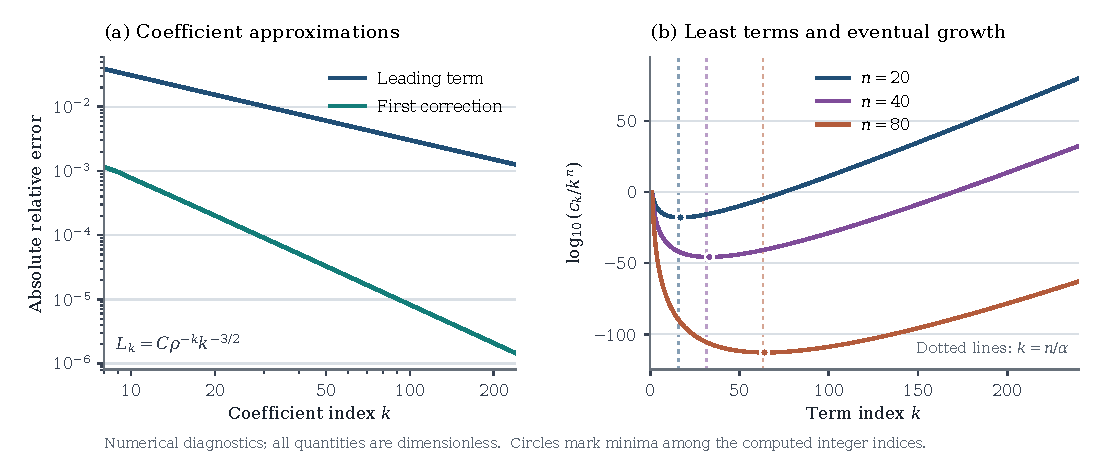
\includegraphics[width=\linewidth]{../reports/gaussian-parity-reductions/figures/14-exact-reductions-moment_asymptotics.pdf}
\caption{Numerical diagnostics for the proved coefficient and moment
asymptotics. Left: absolute relative errors of
\(C\rho^{-k}k^{-3/2}\) and
\(C\rho^{-k}k^{-3/2}(1+\beta_1/k)\), using coefficients computed from
their positive defining recurrence. Right:
\(\log_{10}(c_k/k^n)\) for \(n=20,40,80\). Dotted vertical lines
mark \(k=n/\alpha\); circles mark the sampled minima.
All plotted quantities are dimensionless. The figure illustrates
the theorems and supplies no independent error certificate.}
\label{gaussian:fig:moment-asymptotics}
\end{figure}

\section{Sharp truncation of the log-gamma moment expansion}
Use the constants $\tau,\rho,C$ of the preceding late-coefficient theorem,
and put $\Lambda=-\log\rho$. In this section write $b_k=c_k>0$ for those
positive coefficients, and $\widetilde c_k=(-1)^{k-1}b_k$. The real inverse
$g(t)$ of $1/\Gamma(x)$ on $0\le x\le1$ satisfies $g(t)=-h(-t)$, where
$h(w)=w\Gamma(1-h(w))$ is the earlier inverse germ. Thus
$g(t)=\sum_{k\ge1}\widetilde c_k t^k$ near zero. The moment integral is
\[
 m_n:=M_n/n!=\frac1{\Gamma(n)}\int_0^\infty y^{n-1}g(e^{-y})\,dy.
\]
The first relative coefficient $d_1$ below is the earlier $\beta_1$.
Set $P=\psi'(-\tau)$, $Q=\psi''(-\tau)$, and $R=\psi^{(3)}(-\tau)$; equivalently
$d_1=R/(8P^2)-5Q^2/(24P^3)$.

\begin{lemma}[The dominant inverse singularity]\label{sharp:lem:slit}
The germ $g$ continues to a slit disk of radius greater than $\rho$,
with its only singularity on $|t|=\rho$ at $t=-\rho$, a square-root branch point.
\end{lemma}
\begin{proof}
The positive inverse $h$ has $h(\rho)=\tau$ and is absolutely convergent on
that circle. Its positive coefficients of degrees one and two imply
$|h(t)|<\tau$ at every other point of the circle. With
$\Phi(u)=\Gamma(1-u)$, one then has
$|t\Phi'(h(t))|\le\rho\Phi'(|h(t)|)<\rho\Phi'(\tau)=1$.
The implicit-function theorem continues the inverse across those points.
At $t=\rho$, local inversion at the simple critical point gives a convergent
square-root expansion. Compactness supplies a slightly larger slit disk;
replace $t$ by $-t$ for $g$. This verifies the usual smooth implicit-function
hypotheses directly.\cite{sharp:FS}
\end{proof}
\subsection{A uniform Taylor-remainder lemma}

The next statement is the key passage from fixed-order asymptotics to
optimal truncation. It explicitly crosses the radius of convergence on
the positive real axis; merely summing an infinite Taylor tail there
would be invalid.

\begin{lemma}[Uniform inverse remainder]\label{sharp:lem:inverse-remainder}
For some \(\delta>0\), uniformly for
\(t\in[\rho e^{-\delta},\rho e^\delta]\), put \(r=t/\rho\). Then
\begin{equation}\label{sharp:eq:inverse-remainder}
 \frac{g(t)-\sum_{k=1}^{N-1}\widetilde c_kt^k}{\widetilde c_Nt^N}
 =\frac1{1+r}+\frac{3r}{2N(1+r)^2}+O(N^{-2}).
\end{equation}
On each of the remaining real intervals
\(0<t\leq\rho e^{-\delta}\) and
\(\rho e^\delta\leq t\leq1\), the same normalized remainder is
bounded uniformly in \(N\) sufficiently large.
\end{lemma}

\begin{proof}
The preceding theorem gives a slit disk of continuation for \(g\),
with its only singularity at \(-\rho\).
Choose its outer radius \(R>\rho\), and then \(\delta>0\) so small that
\(\rho e^\delta<R\) and \(\rho e^\delta<1\).
Cauchy's integral formula for \(g(t)\), less its first \(N-1\)
Taylor terms, has kernel \(t^N/(z^N(z-t))\). Deform its contour to the
two banks of the negative cut and an outer contour.
The coefficient \(\widetilde c_N\) uses kernel \(z^{-N-1}\).
On the cut \(z=-s\), the ratio of these kernels, after removing
\(t^N\), is
\[
 \frac{z}{z-t}=\frac{s}{s+t}.
\]
The jump of \(g\) at \(s=\rho\) is a nonzero constant times
\((s-\rho)^{1/2}(1+O(s-\rho))\), with a complete expansion.
The coefficient integral is thus a Watson-type endpoint integral
whose normalized variable \(u=(s-\rho)/\rho\) has
\[
 \langle u\rangle=\frac{3}{2N}+O(N^{-2}),
 \qquad \langle u^2\rangle=O(N^{-2}).
\]
These formulas follow directly by comparing
\(\int_0^\epsilon u^{j+1/2}(1+u)^{-N-1}\dd u\)
with its beta integral extended to infinity. Terms outside a fixed
small neighborhood of zero are exponentially smaller.
Expanding
\[
 \frac{s}{s+t}
 =\frac1{1+r}+\frac{r}{(1+r)^2}u+O(u^2)
\]
proves \eqref{sharp:eq:inverse-remainder}.
The outer contour contributes \(O(R^{-N})\) to the coefficient and
\(O((t/R)^N)\) to the remainder; after normalization these errors are
exponentially small uniformly on the stated compact \(t\)-interval.
This contour argument defines and estimates the actual analytic
remainder on both sides of \(t=\rho\).

It remains to bound the two outer real intervals.
The estimate \(b_k\asymp\rho^{-k}k^{-3/2}\) implies that, below
\(\rho e^{-\delta}\), the absolutely convergent tail is bounded by
a constant times \(b_Nt^N\). Above \(\rho e^\delta\), use
\[
 \sum_{k<N}\frac{b_kt^k}{b_Nt^N}
 \ll\sum_{k<N}(N/k)^{3/2}(\rho/t)^{N-k}.
\]
Splitting at \(k=N/2\) bounds this uniformly by a geometric series
plus an exponentially small term times a polynomial in \(N\).
Furthermore \(0\leq g(t)\leq1\), whereas \(b_Nt^N\) grows
exponentially uniformly on this interval. This proves the last claim.
\end{proof}

\subsection{Sharp optimal truncation}

\begin{theorem}[Half the first omitted term]\label{sharp:thm:optimal-moment}
Let \(n,N\) tend to infinity through positive integers with
\(\eta=N\Lambda-n\) in a fixed bounded interval. Then
\begin{equation}\label{sharp:eq:optimal-moment}
 \boxed{\displaystyle
 m_n-\sum_{k=1}^{N-1}\frac{(-1)^{k-1}b_k}{k^n}
 =\frac{(-1)^{N-1}b_N}{N^n}
 \left(\frac12+\frac{3-2\eta}{8N}+O(N^{-2})\right).}
\end{equation}
The \(O\)-constant is uniform for bounded \(\eta\).
The ratio in parentheses has a complete asymptotic expansion in
\(1/N\), with coefficients computable from the local inverse expansion
and gamma moments.
In particular, taking the nearest integer to \((n+3/2)/\Lambda\)
gives a rigorously justified least-term approximation. The error
eventually has the sign of the first omitted term and is asymptotic
to one half of that term.
\end{theorem}

\begin{proof}
Subtract the finite sum under \eqref{gaussian:eq:moment-inverse}, using
\[
 \frac1{(n-1)!}\int_0^\infty y^{n-1}e^{-ky}\dd y=k^{-n}.
\]
With \(Y\) having the gamma density
\(N^ny^{n-1}e^{-Ny}/(n-1)!\), the error divided by \(\widetilde c_N/N^n\) is
the expectation of the normalized inverse remainder at \(t=e^{-Y}\).

The gamma distribution concentrates at \(\Lambda\):
\[
 \E Y=\frac nN=\Lambda-\frac\eta N,\qquad
 \operatorname{Var}Y=\frac n{N^2}.
\]
For every fixed small \(\delta>0\), its probability outside
\([\Lambda-\delta,\Lambda+\delta]\) is \(O(e^{-a_\delta N})\).
This follows from its moment-generating function
\((1-u/N)^{-n}\) and Chernoff's inequality.
The uniform outer bounds in Lemma~\ref{sharp:lem:inverse-remainder}
therefore make the outer contribution exponentially small.

On the middle interval, the leading kernel is
\[
 L(Y-\Lambda)=\frac1{1+e^{\Lambda-Y}},\qquad
 L(v)=\frac12+\frac v4-\frac{v^3}{48}+O(v^4).
\]
Writing \(V=Y-\Lambda\), its centered gamma moments give
\[
 \E V=-\frac\eta N,\qquad
 \E V^3=O(N^{-2}),\qquad \E V^4=O(N^{-2}),
\]
uniformly for bounded \(\eta\). Thus
\(\E L(V)=1/2-\eta/(4N)+O(N^{-2})\).
It is essential here to use the signed third moment; an absolute
cubic bound alone would lose half a power.
The correction kernel in \eqref{sharp:eq:inverse-remainder} is
\[
 \frac{3e^{-V}}{2N(1+e^{-V})^2}.
\]
Its value at zero is \(3/(8N)\), and its first derivative vanishes
there, so its expectation is \(3/(8N)+O(N^{-2})\).
Adding these terms proves \eqref{sharp:eq:optimal-moment}.
The contour calculation and the Taylor/gamma-moment calculation can
both be continued to arbitrary fixed order. Gamma central moments
are polynomials in \(n\) and \(N^{-1}\); their parity and degree give
integer powers of \(N^{-1}\).
\end{proof}

The theorem strengthens the classical expansion in two ways.
It allows \(N\) to grow linearly with \(n\), and it estimates the
actual error after truncation. The least-term estimate alone would
not justify either conclusion. No global sign assertion for every
\(n,N\) is needed.

\begin{corollary}[Second correction]\label{sharp:cor:moment-second}
Under the hypotheses of Theorem~\ref{sharp:thm:optimal-moment}, the normalized
error has the more precise expansion
\begin{align}
 \frac{m_n-\sum_{k<N}\widetilde c_k/k^n}{\widetilde c_N/N^n}
 &=\frac12+\frac{3-2\eta}{8N}\notag\\
 &\quad+\frac1{N^2}
 \left(\frac{d_1}{4}+\frac{\Lambda(6\eta-13)}{96}\right)
 +O(N^{-3}).\label{sharp:eq:moment-second}
\end{align}
\end{corollary}

\begin{proof}
Here are the additional local coefficients, so that the assertion is
independently reproducible. Let \(v=B-\tau\), and use \(P,Q,R\)
from \eqref{sharp:lem:slit}. The characteristic inverse satisfies
\[
 \log\frac{B/\Gamma(1-B)}{\rho}
 =-\frac{P}{2}v^2+\frac{Q}{6}v^3-\frac{R}{24}v^4+O(v^5).
\]
Putting \(w=\sqrt{1-t/\rho}\) and
\(\alpha_*=\sqrt{2/P}\), inversion gives
\[
 B(t)=\tau-\alpha_* w+\frac{Q}{3P^2}w^2+\mu w^3+O(w^4),
 \qquad
 D:=\frac{\mu}{\alpha_*}
 =-\frac14+\frac{R}{12P^2}-\frac{5Q^2}{36P^3}.
\]
Thus the positive cut density for \(B\) is
\((\alpha_*/\pi)u^{1/2}(1+Du+O(u^2))\), where \(u=t/\rho-1\).
Transfer gives \(d_1=3/8+3D/2\), proving
\eqref{sharp:lem:slit} as well. The normalized endpoint moments are
\[
 \langle u\rangle=\frac{3}{2N}
       +\frac{9/4+3D/2}{N^2}+O(N^{-3}),\qquad
 \langle u^2\rangle=\frac{15}{4N^2}+O(N^{-3}),\qquad
 \langle u^3\rangle=O(N^{-3}).
\]
They follow from beta integrals and the displayed cut density.
The coefficient of \(N^{-2}\) in the inverse remainder at \(r=t/\rho\)
is therefore
\[
 K_2(r)=\frac{r}{(1+r)^2}\left(\frac94+\frac{3D}{2}\right)
                    -\frac{15r}{4(1+r)^3},\qquad K_2(1)=d_1/4.
\]
For the gamma average, put
\(K_1(v)=3e^{-v}/[2(1+e^{-v})^2]\) and \(V=Y-\Lambda\).
Taylor expansion through degree five, using
\(\E|V|^6=O(N^{-3})\), gives
\[
 \E L(V)=\frac12-\frac{\eta}{4N}
       +\frac{\Lambda(3\eta-2)}{48N^2}+O(N^{-3}),\qquad
 \E K_1(V)=\frac38-\frac{3\Lambda}{32N}+O(N^{-2}).
\]
For example \(\E V^3=\Lambda(2-3\eta)N^{-2}+O(N^{-3})\);
the signed fifth moment is \(O(N^{-3})\).
Also \(\E K_2(e^{-V})=K_2(1)+O(N^{-1})\).
The uniform outer bound again makes all outer contributions
exponentially small. Combining the three terms proves
\eqref{sharp:eq:moment-second}.
\end{proof}

\begin{figure}[t]
 \centering
 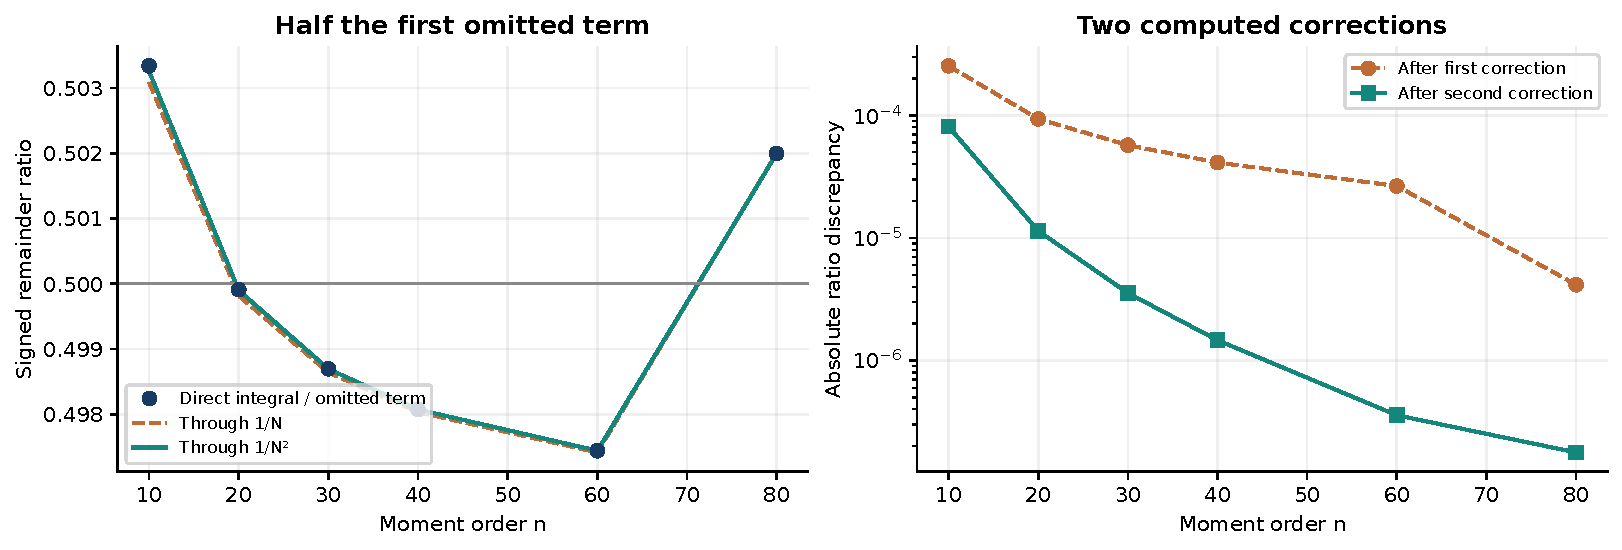
\includegraphics[width=\textwidth]{../reports/reflection-euler-tornheim/figures/moment_remainders.pdf}
 \caption{The signed error divided by the first omitted term, at a
 truncation near \((n+3/2)/\Lambda\). The first-correction formula tracks
 the small changes caused by rounding the truncation index. The plot is
 numerical corroboration; Theorem~\ref{sharp:thm:optimal-moment} supplies the proof.}
 \label{sharp:fig:moments}
\end{figure}

\subsection{A convergent identity with an explicit tail bound}

An asymptotic series should not be used as an infinite exact sum.
The same inverse coordinate gives an exact convergent alternative.

\begin{proposition}[Cutoff identity]\label{sharp:prop:cutoff}
For \(n\geq1\) and \(Y>\Lambda\),
\begin{equation}\label{sharp:eq:cutoff}
 m_n=\frac1{(n-1)!}\int_0^Y y^{n-1}g(e^{-y})\dd y
      +\sum_{k\geq1}\frac{\widetilde c_k}{k^n}Q(n,kY),
 \qquad
 Q(n,z)=e^{-z}\sum_{j=0}^{n-1}\frac{z^j}{j!}.
\end{equation}
The sum is absolutely convergent. If \(Y>\log4\), the absolute tail
after \(k=K\) is at most
\begin{equation}\label{sharp:eq:cutoff-bound}
 \frac{(4e^{-Y})^{K+1}}{2(1-4e^{-Y})}
 \sum_{j=0}^{n-1}\frac{Y^j}{j!(K+1)^{n-j}}.
\end{equation}
\end{proposition}

\begin{proof}
Split \eqref{gaussian:eq:moment-inverse} at \(Y\), substitute the convergent inverse
series on the tail, and integrate term by term.
The coefficient growth theorem proves absolute convergence.
For the elementary explicit bound, note that
\[
 \frac{1/2}{\Phi(1/2)}=\frac1{2\sqrt\pi}>\frac14.
\]
The smaller solution to \(B=t\Phi(B)\) at \(t=1/4\) is therefore
less than \(1/2\); equivalently \(B(1/4)<1/2\).
Positivity gives \(b_k\leq4^k/2\).
For \(k>K\) and \(j\leq n-1\), \(k^{j-n}\leq(K+1)^{j-n}\).
The geometric tail now gives \eqref{sharp:eq:cutoff-bound}.
\end{proof}

The numerical implementation uses ordinary high-precision arithmetic
and explicitly distinguishes analytic truncation bounds from interval
rounding bounds. Formula \eqref{sharp:eq:cutoff} is also suitable for a future
ball-arithmetic evaluator: the finite inverse integral and all constant
evaluations can be enclosed separately.


% Parent document supplies amsmath, amssymb, amsthm, and theorem environments.
% Bibliography key ACEMKM is specified in gamma_provenance.txt.
\section{Reflected log-gamma moments and their late coefficients}
\label{reflected:sec:reflected-moments}

Set $f(x)=\log\Gamma(x)$ for $0<x<1$, and define
\[
 M_{n,m}=\int_0^1 f(x)^n f(1-x)^m\,dx,
 \qquad n,m\in\mathbb Z_{\ge0}.
\]
These integrals already occur as $T_{n+m,n}$ in
Amdeberhan et al.\ \cite[Section~5]{gaussian:ACEMKM}.  Their symmetry
$M_{n,m}=M_{m,n}$ and the identities obtained by expanding Euler's
reflection formula are therefore classical.  The asymptotic question here
is different: keep the reflected exponent $m$ fixed and let $n$ tend to
infinity.  The factor $f(1-x)^m$ vanishes to order $m$ at the endpoint
that produces the factorial growth.  This shifts the first exponential
scale from $1$ to $m+1$ without removing the eventual divergence of the
full expansion.  Theorem~\ref{reflected:gam:thm:late} identifies its late terms,
including their signs and the first relative correction.

\subsection{The meromorphic transform and all finite asymptotic orders}

Put
\[
 B(x)=\log\Gamma(1-x)
 =\gamma x+\sum_{j\ge2}\frac{\zeta(j)}j x^j,
 \qquad |x|<1,
\]
where $\gamma$ is Euler's constant.  For $k\ge1$ define
\begin{equation}\label{reflected:gam:eq:residue-coefficients}
 A_{k,m}=\frac1k[x^{k-1}]\exp\{kB(-x)\}B(x)^m.
\end{equation}
The convention $B(x)^0=1$ is in force.  In particular $A_{k,m}=0$
when $k\le m$.  Every coefficient is a finite polynomial over
$\mathbb Q$ in $\gamma,\zeta(2),\ldots,\zeta(k-1)$.

\begin{theorem}[Reflected moment expansion]\label{reflected:gam:thm:expansion}
For each fixed integer $m\ge0$, the function
\[
 F_m(z)=\int_0^1\Gamma(x)^z f(1-x)^m\,dx
\]
is holomorphic for $\operatorname{Re}z<m+1$, has Taylor expansion
\[
 F_m(z)=\sum_{n\ge0}\frac{M_{n,m}}{n!}z^n
 \qquad (|z|<m+1),
\]
and extends meromorphically to $\mathbb C$.  Its only possible poles
are simple poles at integers $k\ge m+1$, with
\begin{equation}\label{reflected:gam:eq:poles}
 \operatorname*{Res}_{z=k}F_m(z)=-kA_{k,m}.
\end{equation}
The first pole is present.  For every fixed integer $K\ge m+1$,
\begin{equation}\label{reflected:gam:eq:fixed-expansion}
 \frac{M_{n,m}}{n!}
 =\sum_{k=m+1}^{K}\frac{A_{k,m}}{k^n}
   +O_{m,K}\bigl((K+1)^{-n}\bigr),\qquad n\longrightarrow\infty.
\end{equation}
Consequently
\begin{equation}\label{reflected:gam:eq:leading}
 M_{n,m}\sim \frac{\gamma^m n!}{(m+1)^{n+1}}.
\end{equation}
\end{theorem}

\begin{proof}
As $x\downarrow0$, $f(x)=-\log x+O(x)$ and
$B(x)=\gamma x+O(x^2)$.  At the other endpoint,
$f(x)=O(1-x)$ and $f(1-x)=O(1+|\log(1-x)|)$.
These estimates prove absolute convergence and compact domination in
the asserted half-plane, including after any number of differentiations
in $z$.  They also justify the Taylor expansion near zero.

Fix $0<a<1$ and an integer $J\ge1$.  Taylor expansion in $x$ gives
\[
 \Gamma(1+x)^z B(x)^m
 =\sum_{j=0}^{J-1}b_{j,m}(z)x^j+x^J E_{J,m}(x,z),
\]
where each $b_{j,m}$ is an entire function of $z$, and the remainder is
uniformly bounded for $0\le x\le a$ and $z$ in compact sets.
The integral over $[0,a]$ is therefore
\[
 \sum_{j=0}^{J-1}\frac{b_{j,m}(z)a^{j+1-z}}{j+1-z}
 +\int_0^a x^{J-z}E_{J,m}(x,z)\,dx.
\]
The last integral is holomorphic for $\operatorname{Re}z<J+1$.
The integral over $[a,1]$ is entire, since its logarithmic singularity
at $1$ is integrable uniformly for $z$ in compact sets.  Letting $J$
increase gives the continuation.  At $z=k$ its residue is
$-b_{k-1,m}(k)=-kA_{k,m}$.  Since $B(x)^m$ starts with
$\gamma^m x^m$, the first nonzero coefficient is
$A_{m+1,m}=\gamma^m/(m+1)>0$.

For the asymptotic assertion, subtract the polar functions
\[
 \sum_{k=m+1}^{K+1}\frac{kA_{k,m}}{k-z}
\]
from $F_m(z)$.  The difference is holomorphic on $|z|<K+2$.
Cauchy's estimate on any circle $K+1<R<K+2$ bounds its $n$th Taylor
coefficient by $O_{m,K,R}(R^{-n})$.  Restoring the term at $K+1$
proves \eqref{reflected:gam:eq:fixed-expansion}, even if that particular coefficient
happens to vanish.  Taking $K=m+1$ proves \eqref{reflected:gam:eq:leading}.
\end{proof}

The first three coefficients are explicit.  Write $k=m+3$ in the last line:
\begin{align}
 A_{m+1,m}&=\frac{\gamma^m}{m+1},\label{reflected:gam:eq:first-three}\\
 A_{m+2,m}&=\frac{\gamma^{m-1}}{m+2}
 \left(\frac{m\zeta(2)}2-(m+2)\gamma^2\right),\notag\\
 A_{m+3,m}&=\frac{\gamma^m}{k}
 \left\{\frac{m\zeta(3)}{3\gamma}
 +\frac{m(m-1)\zeta(2)^2}{8\gamma^2}
 +\frac{k(1-m)\zeta(2)}2+\frac{k^2\gamma^2}2\right\}.\notag
\end{align}
These displays also apply to $m=0$, since $\gamma>0$ and factors of
$m$ remove the superfluous terms.  For example,
\begin{align*}
 \frac{M_{n,1}}{n!}
 &=\frac{\gamma}{2^{n+1}}
 +\frac{\zeta(2)/2-3\gamma^2}{3^{n+1}}
 +\frac{\zeta(3)/3+8\gamma^3}{4^{n+1}}+O(5^{-n}),\\
 \frac{M_{n,2}}{n!}
 &=\frac{\gamma^2}{3^{n+1}}
 +\frac{\gamma\zeta(2)-4\gamma^3}{4^{n+1}}+O(5^{-n}).
\end{align*}
The second displayed correction is positive, whereas the corresponding
correction for $m=1$ is negative.  Thus strict alternation from the first
term cannot be imported from the unreflected family.  The two signs can,
for instance, be checked using the elementary enclosures
$0.577<\gamma<0.578$ and $1.644<\zeta(2)<1.646$.
Eventual alternation has a different, precise rule.

\subsection{Late coefficients and a universal inverse-gamma scale}

Let $\phi(u)=\Gamma(1-u)$ and $D=u\,d/du$.  Define $\tau\in(0,1)$ by
\begin{equation}\label{reflected:gam:eq:critical}
 D\log\phi(\tau)=-\tau\psi(1-\tau)=1,
\end{equation}
and put
\begin{equation}\label{reflected:gam:eq:constants}
 \rho=\frac{\tau}{\phi(\tau)},\quad
 v=D^2\log\phi(\tau)=1+\tau^2\psi'(1-\tau),\quad
 C=\frac{\tau}{\sqrt{2\pi v}},\quad
 b=-\log\Gamma(1+\tau).
\end{equation}
The equation for $\tau$ has a unique solution: its left side equals
$\gamma u+\sum_{j\ge2}\zeta(j)u^j$, which is strictly increasing from
zero to infinity.  Also $0<\rho<1$ and $b>0$, the latter by strict
log-convexity of $\Gamma$ between $1$ and $2$.  Numerically,
$\tau=0.5040830082\ldots$ and $\rho=0.2821158090\ldots$.
Only the exact definitions are used below.

\begin{theorem}[Late reflected coefficients]\label{reflected:gam:thm:late}
For every fixed nonnegative integer $m$,
\begin{equation}\label{reflected:gam:eq:late}
 A_{k,m}=(-1)^{k+m-1}C b^m\rho^{-k}k^{-3/2}
 \left(1+\frac{\beta_m}{k}+O_m(k^{-2})\right).
\end{equation}
There is a full asymptotic expansion in integer powers of $1/k$.
To specify the first correction, set
$G(u)=\log\Gamma(1+u)$, $H_m(u)=G(u)^m$, and
$\kappa_j=D^j\log\phi(\tau)$.  All quantities on the right below
are evaluated at $u=\tau$:
\begin{equation}\label{reflected:gam:eq:beta}
 \beta_m=
 -\frac{(D+1)^2H_m}{2vH_m}
 +\frac{\kappa_3(D+1)H_m}{2v^2H_m}
 +\frac{\kappa_4}{8v^2}
 -\frac{5\kappa_3^2}{24v^3}.
\end{equation}
In particular, every sufficiently large possible pole in
Theorem~\ref{reflected:gam:thm:expansion} is present.  More explicitly,
\[
 \operatorname{Res}_{z=k}F_m(z)
 =(-1)^{k+m}C b^m\rho^{-k}k^{-1/2}
   \left(1+\frac{\beta_m}{k}+O_m(k^{-2})\right),
\]
so the eventual residue sign is $(-1)^{k+m}$.  For every fixed real $n$, the formal series
$\sum_{k\ge m+1}A_{k,m}/k^n$ diverges because its terms do not tend to zero.
\end{theorem}

\begin{proof}
Replacing $x$ by $-u$ in \eqref{reflected:gam:eq:residue-coefficients} gives
\[
 A_{k,m}=\frac{(-1)^{k-1}}k[u^{k-1}]\phi(u)^k H_m(u).
\]
The function $H_m$ is holomorphic for $|u|<1$.  If
$\phi(u)=\sum_{j\ge0}a_ju^j$, all the $a_j$ are strictly positive,
since $\log\phi$ has positive coefficients.  Thus
\[
 p_j=\frac{a_j\tau^j}{\phi(\tau)}
\]
is a probability distribution with exponential moments, mean one,
variance $v>0$, and positive mass at both $0$ and $1$.  It follows
that the function
\[
 Q(t)=\frac{\phi(\tau e^{it})}{\phi(\tau)}e^{-it}
\]
has modulus strictly less than one for $0<|t|\le\pi$, while
\[
 \log Q(t)=-\frac v2t^2-\frac{i\kappa_3}6t^3
 +\frac{\kappa_4}{24}t^4+O(t^5)
\]
near zero.  Cauchy's coefficient formula becomes
\begin{equation}\label{reflected:gam:eq:cauchy}
 A_{k,m}=
 \frac{(-1)^{k-1}\tau\rho^{-k}}{2\pi k}
 \int_{-\pi}^{\pi}Q(t)^k e^{it}H_m(\tau e^{it})\,dt.
\end{equation}

Fix a sufficiently small $\delta>0$.  On $\delta\le|t|\le\pi$
the integral is $O(q^k)$ for some $q<1$.  On
$k^{-2/5}\le|t|\le\delta$ it is $O(e^{-c k^{1/5}})$, because
$|Q(t)|\le e^{-ct^2}$.  The analytic amplitude is bounded on the
whole circle.  On the remaining interval set $t=y/\sqrt{k}$.
Gaussian domination and Taylor expansion to any fixed order, with
an analytic remainder, give a full expansion.  Odd terms integrate
to zero, so only integer powers of $1/k$ occur.  The leading integral is
\[
 H_m(\tau)\sqrt{\frac{2\pi}{vk}}
 =(-1)^m b^m\sqrt{\frac{2\pi}{vk}},
\]
which proves the leading term in \eqref{reflected:gam:eq:late}.

For the first correction, the amplitude derivatives at $t=0$ are
$H_m$, $i(D+1)H_m$, and $-(D+1)^2H_m$.
The Gaussian moments of degrees $2$, $4$, and $6$ contribute,
respectively, the amplitude's quadratic term, the amplitude--cubic
cross term together with the quartic phase term, and the square of
the cubic phase term.  Their normalized sum is exactly
\eqref{reflected:gam:eq:beta}.  Expanding two further even orders gives a
relative $O_m(k^{-2})$ remainder after the displayed correction.
Since $C b^m>0$ and $\rho<1$, the assertions about nonvanishing,
signs, and divergence follow at once.
\end{proof}

This proof uses the circle $|u|=\tau$ and a strict modulus inequality;
it does not presume a classification of all complex critical values
of the reciprocal gamma function.  The same circle governs every fixed
reflected exponent.  With $\alpha=-\log\rho$, the continuous minimum
of the leading term magnitude $\rho^{-k}k^{-n-3/2}$ occurs at
$k=(n+3/2)/\alpha$.  A least-term calculation alone does not bound the
remainder.  The next result supplies an explicit bound with a growing
number of terms.

\subsection{An effective remainder despite the initial sign changes}

\begin{theorem}[Explicit reflected truncation bound]\label{reflected:gam:thm:effective}
Let $m\ge0$, $n\ge1$, and $K\ge1$ be integers, put
$\alpha=-\log\rho$ and $T_m=\tau B(\tau)^m$, and suppose $K\alpha<n$.
With
\[
 R^{(m)}_{n,K}=\frac{M_{n,m}}{n!}
             -\sum_{k=1}^K\frac{A_{k,m}}{k^n},
 \qquad \Gamma(n,s)=\int_s^\infty t^{n-1}e^{-t}\,dt,
\]
one has the entirely explicit estimate
\begin{align}\label{reflected:gam:eq:effective}
 |R^{(m)}_{n,K}|\le{}&\frac{\alpha^n}{n!}
 \left(m!+\frac{nT_m}{n-K\alpha}\right)\notag\\
 &+\frac{T_m\rho^{-K-1}}{(K+1)^n}
          \frac{\Gamma(n,(K+1)\alpha)}{\Gamma(n)}.
\end{align}
If $n\ge\max\{2,4\alpha^2\}$ and
$K=\lfloor n/\alpha-\sqrt n\rfloor$, then $K\ge1$ and
\begin{equation}\label{reflected:gam:eq:optimized}
 |R^{(m)}_{n,K}|\le
 \left(\frac{m!}{\sqrt{2\pi n}}+
       \frac{T_m}{\alpha\sqrt{2\pi}}+T_m e^{2\alpha^2}\right)
 \left(\frac{e\alpha}{n}\right)^n.
\end{equation}
This bound holds for every $m$, but no useful uniform relative error is
asserted when $m$ grows with $n$.
\end{theorem}
\begin{proof}
The function $f$ decreases from infinity to zero on $(0,1]$:
$\psi'(x)>0$ and $\psi(1)=-\gamma<0$.  Let $x(y)$ denote its inverse,
and set $W_m(x)=\int_0^x B(t)^m\,dt$.  Tonelli's theorem applied to
$f(x)^n=n\int_0^{f(x)}y^{n-1}\,dy$ gives
\begin{equation}\label{reflected:gam:eq:layercake}
 \frac{M_{n,m}}{n!}
 =\frac1{\Gamma(n)}\int_0^\infty y^{n-1}W_m(x(y))\,dy.
\end{equation}

Let $h(q)$ be the local solution of $h=q\phi(h)$ with $h(0)=0$.
Lagrange inversion gives positive coefficients
\[
 h(q)=\sum_{k\ge1}c_kq^k,
 \qquad c_k=\frac1k[u^{k-1}]\phi(u)^k.
\]
The $m=0$ case of Theorem~\ref{reflected:gam:thm:late} proves that its radius
is $\rho$ and that the series converges absolutely on $|q|\le\rho$.
The map $u\mapsto u/\phi(u)$ increases strictly from $0$ to $\rho$
on $[0,\tau]$, so inversion along this interval and continuity imply
$h(\rho)=\tau$.  No other inverse branch is used.

Lagrange--B\"urmann inversion now gives
\[
 W_m(x(y))=\sum_{k\ge1}A_{k,m}e^{-ky}
 \qquad(y\ge\alpha).
\]
Indeed $x(y)=-h(-e^{-y})$ initially for large $y$, and then throughout
$y>\alpha$ by analytic continuation along the strictly monotone real
inverse.  The endpoint follows by absolute convergence.  To prove that
convergence and obtain its quantitative majorant, define
\[
 d_{k,m}=\frac1k[u^{k-1}]\phi(u)^k B(u)^m\ge0.
\]
Coefficientwise absolute values in $B(-u)^m$ are $B(u)^m$.
Consequently $|A_{k,m}|\le d_{k,m}$, while another application of
Lagrange--B\"urmann gives
\[
 \sum_{k\ge1}d_{k,m}\rho^k=W_m(h(\rho))=W_m(\tau)
 \le\tau B(\tau)^m=T_m.
\]
Here $B$ has positive Taylor coefficients and is increasing on $[0,\tau]$.
Thus on $y\ge\alpha$,
\[
 \left|W_m(x(y))-\sum_{k=1}^K A_{k,m}e^{-ky}\right|
 \le T_m\rho^{-K-1}e^{-(K+1)y}.
\]
Its integral in \eqref{reflected:gam:eq:layercake} is the second term of
\eqref{reflected:gam:eq:effective}.

On $0\le y\le\alpha$, use $0\le W_m(x(y))\le M_{m,0}\le m!$.
The last inequality follows from
$0\le\log\Gamma(x)\le-\log x$, since log-convexity gives
$\Gamma(1+x)\le1$ for $0\le x\le1$.  Also, for $k\le K$,
\[
 \int_0^\alpha y^{n-1}e^{-ky}\,dy
 \le\frac{\alpha^n e^{-k\alpha}}{n-k\alpha}.
\]
This follows by differentiating $y^ne^{-ky}$ and using
$n-ky\ge n-k\alpha>0$.  Summing with
$\sum|A_{k,m}|\rho^k\le T_m$ proves the first term of
\eqref{reflected:gam:eq:effective}.

For the stated choice of $K$, $n-K\alpha\ge\alpha\sqrt n$ and
$\theta=(K+1)\alpha/n$ lies in $[1/2,1]$.
The inequality $\theta-1-\log\theta\le2(1-\theta)^2$ gives
\[
 \rho^{-K-1}(K+1)^{-n}
 \le e^{2\alpha^2}(e\alpha/n)^n.
\]
Finally, $\Gamma(n,s)\le\Gamma(n)$ and
$n!\ge\sqrt{2\pi n}(n/e)^n$ yield \eqref{reflected:gam:eq:optimized}.
\end{proof}

\subsection{Sharp truncation for every fixed reflected exponent}
The reflected coefficient expansion and the sharp inverse remainder now
combine. This statement uses the two incoming developments together;
it is stronger than their separate absolute-bound and unreflected results.
Write $\Lambda=-\log\rho$, and retain $\beta_m$ from
\eqref{reflected:gam:eq:beta}.

\begin{corollary}[Half the first omitted reflected term]
\label{reflected:cor:sharp}
Fix an integer $m\ge0$. Let $n,N\to\infty$ through positive integers,
with $\eta=N\Lambda-n$ in a fixed bounded interval. Then
\begin{align}\label{reflected:eq:sharp}
 \frac{M_{n,m}/n!-\sum_{k=1}^{N-1}A_{k,m}/k^n}{A_{N,m}/N^n}
 ={}&\frac12+\frac{3-2\eta}{8N}\notag\\
 &+\frac1{N^2}\left[\frac{\beta_m}{4}
       +\frac{\Lambda(6\eta-13)}{96}\right]+O_m(N^{-3}),
\end{align}
uniformly for bounded $\eta$. In particular the error eventually has
sign $(-1)^{N+m-1}$ and is asymptotic to half the first omitted term.
The denominator is nonzero for every sufficiently large $N$.
\end{corollary}
\begin{proof}
Set $W_m(x)=\int_0^x B(u)^m\,du$ and $G_m(t)=W_m(g(t))$, where $g$ is
the real inverse used in the preceding sharp-moment section.
Lagrange--B\"urmann inversion gives
$G_m(t)=\sum_{k\ge1}A_{k,m}t^k$ near zero. The layer-cake formula
\eqref{reflected:gam:eq:layercake} becomes
\[
 M_{n,m}/n!=\frac1{\Gamma(n)}\int_0^\infty y^{n-1}G_m(e^{-y})\,dy.
\]
Since $W_m$ is holomorphic on $|x|<1$, it can be composed with the
slit-disk inverse of Lemma~\ref{sharp:lem:slit}. At the dominant point
$g(-\rho)=-\tau$ its derivative is
\[
 W_m'(-\tau)=B(-\tau)^m
       =\bigl(\log\Gamma(1+\tau)\bigr)^m=(-b)^m\ne0.
\]
Thus $G_m$ has the same sole dominant square-root singularity, with a
nonzero leading amplitude. Its late coefficients have the relative
coefficient $\beta_m$ established in Theorem~\ref{reflected:gam:thm:late}.
The Cauchy cut-contour argument in Lemma~\ref{sharp:lem:inverse-remainder}
therefore applies to $G_m$ with the same leading kernel
$1/(1+t/\rho)$ and the same $3/(2N)$ endpoint-moment correction.
The sign of the leading jump cancels against $A_{N,m}$ in this ratio.
The second normalized cut coefficient at $t=\rho$ is $\beta_m/4$,
by the same square-root transfer and beta-moment calculation used in
Corollary~\ref{sharp:cor:moment-second}.

The outer real-interval bounds also persist. Above the convergence
radius, the finite coefficient sum is bounded using
$|A_{k,m}|\asymp_m\rho^{-k}k^{-3/2}$, while $0\le G_m(t)\le m!$ for
$0\le t\le1$. The finitely many exceptional early coefficients contribute
only an exponentially small term after normalization. Below the radius,
the absolute Taylor tail gives the corresponding uniform bound.
Average the normalized remainder against the gamma density with shape
$n$ and rate $N$. Its signed moments are exactly those used in the
unreflected calculation. The first two corrections are consequently
\eqref{reflected:eq:sharp}, with $d_1$ replaced by $\beta_m$; the analytic
cut expansion and moments through degree six give the stated uniform
$O_m(N^{-3})$ remainder. Eventual nonvanishing and the sign follow from
\eqref{reflected:gam:eq:late}.
\end{proof}
This fixed-$m$ corollary does not supply uniform relative estimates when
$m$ grows with $n$. That joint regime remains a separate problem.

\subsection{An exact identity coupling all reflected residues}

The coefficients across different $m$ satisfy a finite identity in which
Euler's constant and all odd zeta values cancel.

\begin{proposition}[Reflection sum for the residues]\label{reflected:gam:prop:residue-sum}
For every integer $k\ge1$,
\begin{equation}\label{reflected:gam:eq:residue-sum}
 \sum_{m=0}^{k-1}\frac{k^m}{m!}A_{k,m}
 =\begin{cases}
 0,&k\text{ even},\\[2pt]
 \displaystyle\frac{\pi^{k-1}}{k\,2^{k-1}}
 \binom{k-1}{(k-1)/2},&k\text{ odd}.
 \end{cases}
\end{equation}
\end{proposition}
\begin{proof}
Because $B(x)^m$ has order $m$, extending the sum over $m$ to infinity
does not affect $[x^{k-1}]$.  Euler's reflection formula gives
\[
 \sum_{m=0}^{k-1}\frac{k^m}{m!}A_{k,m}
 =\frac1k[x^{k-1}]\bigl(\Gamma(1+x)\Gamma(1-x)\bigr)^k
 =\frac1k[x^{k-1}]\left(\frac{\pi x}{\sin\pi x}\right)^k.
\]
The coefficient is zero for even $k$.  For odd $k$, compute it as
the residue at $x=0$ of $(\pi/\sin\pi x)^k\,dx$.
The local change of variable $t=\sin\pi x$ gives
\[
 [x^{k-1}]\left(\frac{\pi x}{\sin\pi x}\right)^k
 =\pi^{k-1}[t^{k-1}](1-t^2)^{-1/2},
\]
and the binomial expansion proves \eqref{reflected:gam:eq:residue-sum}.
\end{proof}

For example, the cases $k=2,3$ read
$A_{2,0}+2A_{2,1}=0$ and
$A_{3,0}+3A_{3,1}+\tfrac92 A_{3,2}=\pi^2/6$.
They are exact identities among the asymptotic coefficients, rather
than convergent sums of the moment expansions.  No summation over
the late index $k$ is used.

\subsection{A recorded log-sine conjecture has a formal proof}

There is also a small but useful correction to the logical status of
a claim in the literature.  The author preprint of \cite{gaussian:ACEMKM}
labels a coefficient identity as Conjecture~5.5 and motivates it using
transcendence assumptions on $\log 2$ and $\log\pi$.
For the canonical formal polynomials supplied by the beta integral,
the coefficient identity needs none of those assumptions.  Under the
preprint's assumptions these formal coefficients coincide with its
uniquely specified numerical coefficients, so the result also proves
that stated implication.  We do not assert uniqueness of arbitrary
numerical expressions in zeta values and logarithms, nor priority over
any later treatment.

Define polynomials $\mathcal P_N(X)$ by
\begin{equation}\label{reflected:gam:eq:appell-egf}
 \sum_{N\ge0}\mathcal P_N(X)\frac{z^N}{N!}
 =\exp\left\{Xz+\sum_{j\ge2}
       \frac{(1-2^{1-j})\zeta(j)}jz^j\right\}.
\end{equation}
\begin{proposition}[Unconditional coefficient and translation identities]
\label{reflected:gam:prop:appell}
For $N\ge0$,
\begin{align}
 \int_0^1[-\log\sin(\pi x)]^N\,dx&=\mathcal P_N(\log2),\label{reflected:gam:eq:logsine}\\
 [X^j]\mathcal P_N(X)&=\binom Nj \mathcal P_{N-j}(0),\qquad 0\le j\le N,\notag\\
 \sum_{j=0}^N\binom Nj M_{j,N-j}&=\mathcal P_N(\log(2\pi)).\notag
\end{align}
Moreover, the coefficients admit the finite partition formula
\begin{equation}\label{reflected:gam:eq:appell-partitions}
 \mathcal P_N(X)=N!\!\sum_{r_1+2r_2+\cdots+Nr_N=N}
 \frac{X^{r_1}}{r_1!}
 \prod_{j=2}^N\frac1{r_j!}
 \left(\frac{(1-2^{1-j})\zeta(j)}j\right)^{r_j}.
\end{equation}
\end{proposition}
\begin{proof}
For $\operatorname{Re}z<1$, the beta integral gives
\[
 \int_0^1\sin(\pi x)^{-z}\,dx
 =\frac{\Gamma((1-z)/2)}{\sqrt\pi\,\Gamma(1-z/2)}.
\]
Expanding its logarithm at zero gives the right side of
\eqref{reflected:gam:eq:appell-egf} with $X=\log2$; its degree-$j$ coefficient
for $j\ge2$ is $(1-2^{1-j})\zeta(j)/j$.
Extracting Taylor coefficients proves \eqref{reflected:gam:eq:logsine}.
The factor $e^{Xz}$ gives $[X^j]\mathcal P_N=\binom Nj\mathcal P_{N-j}(0)$ by
formal coefficient extraction.  Euler's reflection formula turns
the sum of mixed moments into the integral of
$(\log\pi-\log\sin\pi x)^N$, which translates $X$ by $\log\pi$.
Expanding each exponential factor separately proves
\eqref{reflected:gam:eq:appell-partitions}.  All formal operations in a fixed
degree involve only finitely many coefficients.
\end{proof}

The constant-column generating function has the additional factorization
\begin{equation}\label{reflected:gam:eq:even-odd-factor}
 \sum_{N\ge0}\mathcal P_N(0)\frac{z^N}{N!}
 =\sqrt{\frac{\tan(\pi z/2)}{\pi z/2}}
 \exp\left\{\sum_{\substack{j\ge3\\j\text{ odd}}}
       \frac{(1-2^{1-j})\zeta(j)}jz^j\right\},
\end{equation}
where the square root is the formal branch with constant term one.
Indeed, multiplying the left side by its value at $-z$ and applying
the reflection formula yields $\tan(\pi z/2)/(\pi z/2)$.
The even logarithmic part is therefore the displayed square root.
This makes the multiplicative factorization of its formal odd-zeta
monomial coefficients explicit, while the even-zeta contribution has
an elementary trigonometric generating function.

\paragraph{Verification and remaining questions.}
The accompanying script \src{code/verify_reflected_moments.py} checks the
three coefficient formulas by exact symbolic arithmetic, checks finite
reflection sums and the formal Appell formulas, and compares independent
quadrature with the fixed-order expansion.  It also compares the late
coefficients with \eqref{reflected:gam:eq:late} and \eqref{reflected:gam:eq:beta}.
The numerical calculations are diagnostics; the preceding analytic and
formal arguments are the proofs.
The fixed-reflected-exponent signed remainder is now supplied by
Corollary~\ref{reflected:cor:sharp}. Uniformity when $m$ increases with
$n$ remains a substantive next question.
In the former regime the endpoint approximation
$B(x)^m\approx\gamma^m x^m$ need not be uniform, so the fixed-$m$
theorem does not settle the simultaneous large-exponent problem.


\section{The Stieltjes layer}\label{integral:sec:stieltjes}

Differentiating $L(s,\chi)=q^{-s}\sum_k\chi(k)\,\zeta(s,k/q)$ at $s=1$ gives the exact
ladder
\[
L'(\chi,1)=-\ln q\;L(1,\chi)-\frac1q\sum_k\chi(k)\,\gamma_1\!\Bigl(\frac{k}{q}\Bigr),
\]
so every Malmsten log-log integral is a statement about \emph{first generalized Stieltjes
constants} $\gamma_1(k/q)$ --- Blagouchine's program, equivalent to Deninger's
$\zeta''(0,a)$ layer via the functional equation.

\begin{result}[even-character Malmsten integral]\label{integral:res:evenchi}
\dps{verified to $10^{-51}$; even character mod 5; $\varphi$ the golden ratio}
\[
\int_0^1\ln\ln\frac1x\cdot\frac{(1-x)(1-x^2)}{1-x^5}\,dx
=-(\gamma+\ln5)\,\frac{2\ln\varphi}{\sqrt5}
-\frac{\gamma_1(\tfrac15)-\gamma_1(\tfrac25)-\gamma_1(\tfrac35)+\gamma_1(\tfrac45)}{5}.
\]
\end{result}

\begin{result}[the parity dichotomy]\label{integral:res:parity}
The dichotomy is empirically sharp. The \emph{odd} $\gamma_1$-combination reduces exactly
as differentiated-Kummer predicts \dps{verified blind}:
\[
\gamma_1\!\bigl(\tfrac13\bigr)-\gamma_1\!\bigl(\tfrac23\bigr)
=-\frac{\pi}{\sqrt3}\Bigl(\gamma+4\ln2-\tfrac12\ln3+4\ln\pi-6\ln\Gamma\bigl(\tfrac13\bigr)\Bigr),
\]
which is \emph{Malmsten's 1846 reflection identity} \cite{bridge:Malmsten} (long misattributed
to Almkvist--Meurman). The even combination did not reduce in the tested standard basket
\dps{PSLQ junk at coefficient height $10^8$ --- honest negative}; pushing Blagouchine's
rational-arguments theorem \cite{bridge:BlagouchineJNT} through it collapses everything except a $\zeta''$-block
\dps{derived and verified to $10^{-50}$}:
\[
\gamma_1\!\bigl(\tfrac15\bigr)-\gamma_1\!\bigl(\tfrac25\bigr)
-\gamma_1\!\bigl(\tfrac35\bigr)+\gamma_1\!\bigl(\tfrac45\bigr)
=\sqrt5\,\Bigl[\zeta''\bigl(0,\tfrac15\bigr)-\zeta''\bigl(0,\tfrac25\bigr)
-\zeta''\bigl(0,\tfrac35\bigr)+\zeta''\bigl(0,\tfrac45\bigr)\Bigr]
-2\sqrt5\,\ln\varphi\,\bigl(\gamma+\ln10\pi\bigr).
\]
\end{result}

The canonical atom for the even layer is thus the even-character $\zeta''(0,l/q)$
combination (Deninger's layer \cite{bridge:Deninger}); Malmsten integrals, even $\gamma_1$-combinations, and even
$L'(\chi,1)$ are all elementary-equivalent to it. Two practical records: Blagouchine's
particular value $\gamma_1(1/4)$ was re-verified exactly against \texttt{mpmath}'s
generalized Stieltjes constants, and the reduction coefficients live in
$\mathbb{Q}(\sqrt q)$ --- rational-coefficient PSLQ baskets \emph{miss} the relation, so a
$\sqrt q$-weighted basket or direct derivation is required.
\section{The common Hurwitz-jet calculus}\label{stieltjes:sec:intro}

The generalized Stieltjes constants $\gamma_n(x)$ are defined by the Laurent
expansion of the Hurwitz zeta function at its pole,
\begin{equation}\label{stieltjes:eq:laurent}
\zeta(s,x)=\frac{1}{s-1}+\sum_{n\ge0}\frac{(-1)^n}{n!}\,\gamma_n(x)\,(s-1)^n ,
\end{equation}
so that $\gamma_0(x)=-\psi(x)$ and $\gamma_n(1)=\gamma_n$ are the classical
Stieltjes constants, $\gamma_0=\gamma$. Although universally called
\emph{constants}, the $\gamma_n(x)$ are real-analytic functions of the
argument on $(0,\infty)$, and it is this function-theoretic point of view we
adopt. Following Blagouchine \cite{stieltjes:BlagouchineRJ,bridge:BlagouchineJNT} we write
\[
\Gamma_{\!n}(p)\;:=\;\int_1^p\gamma_n(x)\,dx ,
\qquad\text{so that }\ \Gamma_{\!n}(1)=0 ,
\]
for the antiderivative normalized at $1$. (The notation is Blagouchine's; the
clash with the Euler $\Gamma$-function is resolved by the subscript, and
indeed $\Gamma_{\!0}(p)=-\ln\Gamma(p)$, as Theorem~\ref{stieltjes:thm:ladder} makes
plain.) Throughout, $\zeta^{(k)}(s_0,a):=\partial_s^k\zeta(s,a)\big|_{s=s_0}$
and $\zeta^{(k)}(s_0):=\zeta^{(k)}(s_0,1)$ denote derivative jets with respect
to the \emph{order}; $\Lambda_q:=\gamma+\ln(2\pi q)$; $H_n=\sum_{i\le n}1/i$ and
$H_n^{(2)}=\sum_{i\le n}1/i^2$ are harmonic numbers; $\Glaisher$ is the
Glaisher--Kinkelin constant, $\ln\Glaisher=\tfrac1{12}-\zeta'(-1)$; and
\[
S_j\Bigl(\frac pq\Bigr):=\sum_{k=1}^{q-1}\sin\frac{2\pi kp}{q}\,
\zeta^{(j)}\Bigl(0,\frac kq\Bigr),
\qquad
S_0\Bigl(\frac pq\Bigr)=\tfrac12\cot\frac{\pi p}{q},
\quad
S_1\Bigl(\frac pq\Bigr)=\sum_{k=1}^{q-1}\sin\frac{2\pi kp}{q}\,\ln\Gamma\Bigl(\frac kq\Bigr)
\]
(the closed forms for $S_0,S_1$ use $\zeta(0,a)=\tfrac12-a$,
$\zeta'(0,a)=\ln\Gamma(a)-\tfrac12\lntwopi$, and
$\sum_k\sin(2\pi kp/q)=0$).

The starting observation is elementary but organizing: differentiating
\eqref{stieltjes:eq:laurent} in $x$ against $\partial_x\zeta(s,x)=-s\,\zeta(s+1,x)$
identifies every derivative and antiderivative of every $\gamma_n$ with a
derivative jet of the Hurwitz zeta function at an \emph{integer} value of
$s$. Antiderivatives live at $s=0$; the functions themselves at $s=1$; their
$x$-derivatives at $s=2$ \cite{stieltjes:Coffey} — a single ladder.

The preceding gamma-integral examples are the first rung of this
calculus. We now prove the integration identity, build its spectral jets,
and use reflection and distribution to compute rational arguments.
All source residuals in this chapter are historical; locally rerun checks
are recorded separately in the verification directory.

\section{Underived Stieltjes grids and character coordinates}
Expanding the Hurwitz distribution identity at $s=1$ gives
\begin{align*}
\sum_{j=0}^{d-1}\gamma_1((x+j)/d)
&=d\gamma_1(x)+d\log d\,\psi(x)-\frac d2\log^2d,\\
\sum_{j=0}^{d-1}\gamma_2((x+j)/d)
&=d\left[\gamma_2(x)-2\log d\,\gamma_1(x)
-\log^2d\,\psi(x)+\frac13\log^3d\right].
\end{align*}
For a nonprincipal character,
\[
L'(1,\chi)=-\log q\,L(1,\chi)
-\frac1q\sum_{p=1}^{q}\chi(p)\gamma_1(p/q).
\]
For a real quadratic character $\chi_D$,
$\zeta_{\mathbb Q(\sqrt D)}(s)=\zeta(s)L(s,\chi_D)$ shows
$L'(1,\chi_D)/L(1,\chi_D)=\gamma_{\mathbb Q(\sqrt D)}-\gamma$,
where the first term is the field's Euler--Kronecker constant.
The source's exact finite matrices for $3\le q\le30$ left
$\varphi(q)/2-1$ coordinates after distribution and first-constant
reflection. Their negative searches constrain the selected baskets,
without proving independence of Euler--Kronecker constants.
The reflection formulas below retain the conductor factor
$\gamma+\log(2\pi q)$: the earlier printed $q=5$ specialization without
$\log5$ was corrected in the source reports.

\section{The ladder}\label{stieltjes:sec:ladder}

\begin{theorem}[antiderivative ladder]\label{stieltjes:thm:ladder}
For $n\ge0$ and $p>0$,
\begin{equation}\label{stieltjes:eq:chain}
\frac{d}{dp}\,\zeta^{(n+1)}(0,p)=(-1)^{n+1}(n+1)\,\gamma_n(p),
\end{equation}
and consequently
\begin{equation}\label{stieltjes:eq:antideriv}
\Gamma_{\!n}(p)=\frac{(-1)^{n+1}}{n+1}\Bigl[\zeta^{(n+1)}(0,p)-\zeta^{(n+1)}(0)\Bigr].
\end{equation}
\end{theorem}

\begin{proof}
Differentiating $\partial_x\zeta(s,x)=-s\,\zeta(s+1,x)$ is legitimate
termwise for $\operatorname{Re}s>1$ and extends by analytic continuation.
Expand both sides around $s=0$: on the right,
$-s\,\zeta(s+1,x)=-s\bigl[\tfrac1s+\sum_k\tfrac{(-1)^k}{k!}\gamma_k(x)s^k\bigr]
=-1-\sum_k\tfrac{(-1)^k}{k!}\gamma_k(x)s^{k+1}$,
whose $s^{n+1}$-coefficient is $(-1)^{n+1}\gamma_n(x)/n!$. On the left the
$s^{n+1}$-coefficient is $\partial_x\zeta^{(n+1)}(0,x)/(n+1)!$. Equating gives
\eqref{stieltjes:eq:chain}; integrating from $1$ to $p$ gives \eqref{stieltjes:eq:antideriv}.
\end{proof}

The differential form \eqref{stieltjes:eq:chain} is Lemma~2 of
Chakraborty--Kanemitsu--Kuzumaki \cite{stieltjes:CKK} (for $n=1$ it is Deninger's
$R'$-law \cite{bridge:Deninger}); the integrated form \eqref{stieltjes:eq:antideriv} is
eq.~(2.16) of Connon \cite{stieltjes:Connon}. For $n=0$,
$\zeta'(0,p)=\ln\Gamma(p)-\tfrac12\lntwopi$ recovers
$\Gamma_{\!0}(p)=-\ln\Gamma(p)$.

\begin{theorem}[interpolation of power sums of logarithms]\label{stieltjes:thm:interp}
For $k\ge1$ and integer $N\ge0$,
\[
\Gamma_{\!k-1}(N+1)\;=\;-\frac1k\sum_{j=1}^{N}\ln^k j .
\]
\end{theorem}

\begin{proof}
From $\zeta(s,N+1)=\zeta(s)-\sum_{j=1}^N j^{-s}$,
$\zeta^{(k)}(0,N+1)=\zeta^{(k)}(0)-\sum_j(-\ln j)^k
=\zeta^{(k)}(0)-(-1)^k\sum_j\ln^k j$. Insert into \eqref{stieltjes:eq:antideriv} with
$n=k-1$.
\end{proof}

Thus $\Gamma_{\!k-1}$ is an analytic interpolant of the power sums
$\sum\ln^k j$ (up to the factor $-1/k$), exactly as $\ln\Gamma$ interpolates
$\ln N!$: the heuristic ``differentiate $1^r+\dots+N^r=\zeta(-r)-\zeta(-r,N+1)$
$k$ times at $r=0$'' becomes precise through
Theorem~\ref{stieltjes:thm:ladder}.

\begin{corollary}[unit translates]\label{stieltjes:cor:translates}
For $k\ge0$ and integer $n\ge1$,
\[
\int_n^{n+1}\gamma_k(x)\,dx=-\frac{\ln^{k+1}n}{k+1};
\qquad\text{in particular }\ \int_1^2\gamma_k(x)\,dx=0 .
\]
\end{corollary}

\noindent
(The case $n=1$ is eqs.~(2.18)--(2.19) of \cite{stieltjes:Connon}.)

\section{Zeta jets and the conversion dictionary}\label{stieltjes:sec:jets}

Making \eqref{stieltjes:eq:antideriv} explicit requires the constants
$\zeta^{(k)}(0)$ and, for the moment evaluations of
Section~\ref{stieltjes:sec:moments}, the jets at negative integers. All of them follow
mechanically from the functional equation
$\zeta(s)=2^s\pi^{s-1}\sin(\pi s/2)\,\Gamma(1-s)\,\zeta(1-s)$
by expanding $\Gamma(1-s)=\exp\bigl(\gamma s+\sum_{k\ge2}\zeta(k)s^k/k\bigr)$
and the Laurent series of $\zeta(1-s)$ at the pole.

\begin{proposition}[jets at $0$]\label{stieltjes:prop:jets0}
With $L:=\lntwopi$,
\begin{align*}
\zeta'(0)&=-\tfrac{L}{2},\\
\zeta''(0)&=\tfrac{\gamma^2}{2}+\gamma_1-\tfrac{\pi^2}{24}-\tfrac{L^2}{2},\\
\zeta'''(0)&=\gamma^3+3\gamma\gamma_1+\tfrac32\gamma_2-\zeta(3)
+\tfrac32\gamma^2L+3\gamma_1L-\tfrac{\pi^2}{8}L-\tfrac{L^3}{2},\\
\zeta^{(4)}(0)&=\tfrac32\gamma^4+4\gamma^3L+6\gamma^2\gamma_1+3\gamma^2L^2
+\tfrac{\pi^2}{4}\gamma^2+12\gamma\gamma_1L+6\gamma\gamma_2
+6\gamma_1L^2+\tfrac{\pi^2}{2}\gamma_1\\
&\quad+6\gamma_2L+2\gamma_3
-\tfrac{L^4}{2}-\tfrac{\pi^2}{4}L^2-4\zeta(3)L-\tfrac{19\pi^4}{480}.
\end{align*}
\end{proposition}

\begin{proposition}[fifth jet at $0$]\label{stieltjes:prop:jets0def}
With $L:=\lntwopi$,
\begin{align*}
\zeta^{(5)}(0)
&=2\gamma^5+\tfrac{15}{2}\,\gamma^4L
+\gamma^3\Bigl(10L^2+\tfrac{5\pi^2}{6}\Bigr)
+\gamma^2\Bigl(5L^3+\tfrac{5\pi^2}{4}\,L+10\,\zeta(3)\Bigr)\\
&\quad+\gamma\gamma_1\Bigl(30L^2+\tfrac{5\pi^2}{2}\Bigr)
+\gamma_1\Bigl(10\gamma^3+30\gamma^2L+10L^3+\tfrac{5\pi^2}{2}\,L+20\,\zeta(3)\Bigr)\\
&\quad+\gamma_2\Bigl(15\gamma^2+30\gamma L+15L^2+\tfrac{5\pi^2}{4}\Bigr)
+\gamma_3\,(10\gamma+10L)+\tfrac52\,\gamma_4\\
&\quad-\zeta(3)\Bigl(10L^2+\tfrac{5\pi^2}{6}\Bigr)-12\,\zeta(5)
-\tfrac{L^5}{2}-\tfrac{5\pi^2}{12}\,L^3-\tfrac{19\pi^4}{96}\,L .
\end{align*}
\end{proposition}

The values $\zeta''(0)$ and $\zeta'''(0)$ are classical (Ramanujan
\cite{stieltjes:Berndt}; Apostol \cite{stieltjes:Apostol85}; Choudhury \cite{stieltjes:Choudhury}).
Apostol's Theorem~3 \cite{stieltjes:Apostol85} in fact gives a closed form of
$\zeta^{(n)}(0)$ at every order, in terms of the Laurent coefficients of
$\Gamma(s)\zeta(s)$ at $s=1$, and prints the example $n=4$ in that
vocabulary; we have not located the fully expanded forms above — nor any
explicit form of $\zeta^{(5)}(0)$ — in print. The pattern continues to
every order by the same expansion, which packages into the following
closed recurrence.

\begin{remark}[explicit recurrence for the jets at $0$]\label{stieltjes:rem:jetrec}
In $\zeta(s)=\chi(s)\,\zeta(1-s)$ with
$\chi(s)=2^s\pi^{s-1}\sin(\pi s/2)\,\Gamma(1-s)$,
the simple zero of $\chi$ at $s=0$ cancels the pole of $\zeta(1-s)$; factor
it out as $\chi(s)=\tfrac{s}{2}\,e^{g(s)}$ with
$g(s):=\ln\bigl(2\chi(s)/s\bigr)
=\ln\bigl[(2\pi)^s\,\tfrac{\sin(\pi s/2)}{\pi s/2}\,\Gamma(1-s)\bigr]$,
analytic on $|s|<1$ and real on $(-1,1)$ (the bracket is positive there),
$g(0)=0$. From $\ln\Gamma(1-s)=\gamma s+\sum_{k\ge2}\zeta(k)s^k/k$ and
$\ln\bigl[\sin(\pi s/2)\big/(\pi s/2)\bigr]=-\sum_{m\ge1}\zeta(2m)(s/2)^{2m}/m$,
\[
g(s)=(\gamma+L)\,s+\sum_{k\ge2}c_k s^k,\qquad
c_k=\frac{\zeta(k)}{k}\cdot\begin{cases}1,&k\ \text{odd},\\
1-2^{1-k},&k\ \text{even},\end{cases}
\]
so $c_2=\tfrac{\pi^2}{24}$, $c_3=\tfrac{\zeta(3)}{3}$,
$c_4=\tfrac{7\pi^4}{2880}$, $c_5=\tfrac{\zeta(5)}{5}$. Since
$s\,\zeta(1-s)=-1+\sum_{m\ge1}\gamma_{m-1}\,s^m/(m-1)!$ is entire, the
Leibniz rule gives
\[
\zeta^{(n)}(0)=\frac12\sum_{k=0}^{n}\binom{n}{k}\,
B_k\bigl(1!\,c_1,2!\,c_2,\dots,k!\,c_k\bigr)\,h_{n-k},
\qquad h_0=-1,\quad h_m=m\,\gamma_{m-1}\ (m\ge1),
\]
where $c_1=\gamma+L$ and $B_k$ is the complete Bell polynomial,
$B_k\bigl(g'(0),\dots,g^{(k)}(0)\bigr)=\bigl(e^{g}\bigr)^{(k)}(0)$: $B_0=1$,
$B_1=c_1$, $B_2=c_1^2+2c_2$, $B_3=c_1^3+6c_1c_2+6c_3$. The cases $n=0,1$
recover $\zeta(0)=-\tfrac12$ and $\zeta'(0)=-\tfrac{L}{2}$; $n=2,\dots,5$
reproduce the two propositions verbatim.
\end{remark}

\begin{proposition}[jets at $-1$ and $-2$]\label{stieltjes:prop:jetsneg}
Expanding the functional equation around $s=-1$ (where $\zeta(2-\varepsilon)$
is regular) and $s=-2$ (a trivial zero) gives, with $L=\lntwopi$:
\begin{align}
\zeta(-1)&=-\tfrac1{12},\qquad
\zeta'(-1)=\frac{\zeta'(2)}{2\pi^2}+\frac{1-\gamma-L}{12},\label{stieltjes:eq:zpm1}\\
\zeta''(-1)&=-\frac{\zeta''(2)}{2\pi^2}+\frac{\zeta'(2)}{\pi^2}(\gamma+L-1)
-\frac{(\gamma+L)^2}{12}+\frac{\gamma+L}{6}+\frac{\pi^2}{144},\label{stieltjes:eq:zppm1}\\
\zeta(-2)&=0,\qquad
\zeta'(-2)=-\frac{\zeta(3)}{4\pi^2},\qquad
\zeta''(-2)=\frac{\zeta(3)}{4\pi^2}\,(3-2\gamma-2L)+\frac{\zeta'(3)}{2\pi^2}.
\label{stieltjes:eq:zm2}
\end{align}
\end{proposition}

\begin{remark}[Glaisher spelling]\label{stieltjes:rem:glaisher}
Since $\ln\Glaisher=\tfrac1{12}-\zeta'(-1)$, eq.~\eqref{stieltjes:eq:zpm1} is
equivalent to
\[
\zeta'(2)=\zeta(2)\bigl(\gamma+\lntwo+\lnpi-12\ln\Glaisher\bigr),
\]
the form returned by Mathematica's
\texttt{FunctionExpand[Zeta$'$[2]]}. Either spelling may be used in all the
moment formulas below; we keep $\zeta'(2),\zeta''(2),\zeta'(3)$ as the
canonical second-layer constants.
\end{remark}

\section{Reflection formulas}\label{stieltjes:sec:reflection}

Hurwitz's formula (see, e.g., \cite[Ch.~12]{stieltjes:ApostolBook}), for $0<p/q<1$,
\[
\zeta\Bigl(1-s,\frac pq\Bigr)
=\frac{2\,\Gamma(s)}{(2\pi q)^{s}}
\sum_{k=1}^{q}\Bigl[\cos\Bigl(\frac{\pi s}{2}-\frac{2\pi kp}{q}\Bigr)\Bigr]
\zeta\Bigl(s,\frac kq\Bigr),
\]
expanded around $s=0$, expresses every $\gamma_n(p/q)$ through the jets
$\zeta^{(j)}(0,k/q)$, $j\le n+1$. Taking the part odd under
$p\mapsto q-p$ isolates the sine sums $S_j$ and yields reflection formulas.
Write
$E(s):=\exp\bigl(-\Lambda_qs+\sum_{k\ge2}(-1)^k\zeta(k)s^k/k\bigr)=\sum_i e_is^i$
for the prefactor expansion
($2\Gamma(s)(2\pi q)^{-s}=\tfrac2s\,E(s)$).

\begin{theorem}[reflection, general mechanism]\label{stieltjes:thm:reflgen}
For $n\ge1$ and $0<p<q$,
\[
\gamma_n\Bigl(\frac pq\Bigr)-\gamma_n\Bigl(1-\frac pq\Bigr)
\;=\;4\,n!\!\!\sum_{i+2l+1+j\,=\,n+1}\!\! e_i\,
\frac{(-1)^l(\pi/2)^{2l+1}}{(2l+1)!}\,\frac{S_j(p/q)}{j!}\,.
\]
Explicitly, with $\Lambda=\Lambda_q=\gamma+\ln 2\pi q$ (the letter
distinguishes it from the Glaisher constant $\Glaisher$):
\begin{align}
\gamma_2\Bigl(\tfrac pq\Bigr)-\gamma_2\Bigl(1-\tfrac pq\Bigr)
&=2\pi S_2-4\pi \Lambda\,S_1+\Bigl(2\Lambda^2+\tfrac{\pi^2}{6}\Bigr)\pi S_0,
\label{stieltjes:eq:refl2}\\
\gamma_3\Bigl(\tfrac pq\Bigr)-\gamma_3\Bigl(1-\tfrac pq\Bigr)
&=2\pi S_3-6\pi \Lambda\,S_2+\Bigl(6\Lambda^2+\tfrac{\pi^2}{2}\Bigr)\pi S_1
-\Bigl(2\Lambda^3+\tfrac{\pi^2}{2}\Lambda+4\zeta(3)\Bigr)\pi S_0,
\label{stieltjes:eq:refl3}\\
\gamma_4\Bigl(\tfrac pq\Bigr)-\gamma_4\Bigl(1-\tfrac pq\Bigr)
&=2\pi S_4-8\pi \Lambda\,S_3+\bigl(12\Lambda^2+\pi^2\bigr)\pi S_2
-\bigl(8\Lambda^3+2\pi^2\Lambda+16\zeta(3)\bigr)\pi S_1\notag\\
&\qquad
+\Bigl(2\Lambda^4+\pi^2\Lambda^2+16\Lambda\,\zeta(3)+\tfrac{19\pi^4}{120}\Bigr)\pi S_0 .
\label{stieltjes:eq:refl4}
\end{align}
\end{theorem}

\begin{proof}
Split the cosine, $\cos(\pi s/2-\theta)=\cos(\pi s/2)\cos\theta
+\sin(\pi s/2)\sin\theta$. Under $p\mapsto q-p$ the cosine sums are even and
the sine sums odd, so the odd part of $\zeta(1-s,p/q)$ equals
$\tfrac2s\,E(s)\sin(\pi s/2)\sum_j S_j\,s^j/j!$. By \eqref{stieltjes:eq:laurent},
$\zeta(1-s,p/q)=-\tfrac1s+\sum_n\gamma_n(p/q)\,s^n/n!$, whose odd part has
$s^n$-coefficient $\tfrac1{2\,n!}\bigl[\gamma_n(p/q)-\gamma_n(1-p/q)\bigr]$.
Matching coefficients of $s^{n}$ (i.e.\ $s^{n+1}$ of
$E\cdot\sin\cdot\sum S_js^j/j!$) gives the general formula; instantiating
$e_0=1$, $e_1=-\Lambda$, $e_2=\tfrac{\Lambda^2}2+\tfrac{\pi^2}{12}$,
$e_3=-\tfrac{\Lambda^3}6-\tfrac{\pi^2}{12}\Lambda-\tfrac{\zeta(3)}3$,
$e_4=\tfrac{\Lambda^4}{24}+\tfrac{\pi^2}{24}\Lambda^2+\tfrac{\zeta(3)}3\Lambda
+\tfrac{\pi^4}{288}+\tfrac{\pi^4}{360}$ yields
\eqref{stieltjes:eq:refl2}--\eqref{stieltjes:eq:refl4}.
\end{proof}

Formula \eqref{stieltjes:eq:refl2} is eq.~(89) of Blagouchine \cite{bridge:BlagouchineJNT},
where a footnote records that it also appears in unpublished work of
D.~Connon; \eqref{stieltjes:eq:refl3} and \eqref{stieltjes:eq:refl4} appear to be new. The same
expansion, one order down, recovers Malmsten's reflection formula for
$\gamma_1$ \cite{bridge:BlagouchineJNT}; an elementary alternative proof of that
$n=1$ case, via Kummer's Fourier expansion of $\ln\Gamma$ rather than
Hurwitz's functional equation, is given by Kouba \cite{stieltjes:Kouba}. For $q=3$
and $q=4$ the sums collapse
($S_j(\tfrac13)=\tfrac{\sqrt3}{2}\bigl[\zeta^{(j)}(0,\tfrac13)-\zeta^{(j)}(0,\tfrac23)\bigr]$,
$S_j(\tfrac14)=\zeta^{(j)}(0,\tfrac14)-\zeta^{(j)}(0,\tfrac34)$), so
\eqref{stieltjes:eq:refl2}--\eqref{stieltjes:eq:refl4} can be \emph{inverted} to express the odd
jet differences through the Stieltjes differences
$\gamma_n(p)-\gamma_n(1-p)$ — the key to Section~\ref{stieltjes:sec:values}.

\section{Moments}\label{stieltjes:sec:moments}

\begin{theorem}[Hurwitz transform and variants]\label{stieltjes:thm:transform}
For $m\ge1$ and $\operatorname{Re}s<1$,
\begin{equation}\label{stieltjes:eq:transform}
\int_0^1 x^m\,\zeta(s,x)\,dx
=-\sum_{j=1}^{m}\frac{m!}{(m-j+1)!}\,
\frac{\zeta(s-j)}{(s-1)(s-2)\cdots(s-j)} ,
\end{equation}
and $\int_0^1\zeta(s,x)\,dx=0$. The same recursion with boundary terms
$\zeta(\sigma,\tfrac12)=(2^\sigma-1)\zeta(\sigma)$ and
$\zeta(\sigma,2)=\zeta(\sigma)-1$ gives the analogous closed forms for
$\int_{1/2}^1$ and $\int_1^2$.
\end{theorem}

\begin{proof}
Since $\zeta(s,x)=-\partial_x\zeta(s-1,x)/(s-1)$, integration by parts gives
$I_m(s)=-\zeta(s-1)/(s-1)+\tfrac{m}{s-1}I_{m-1}(s-1)$ for $m\ge1$.
In the stated half-plane the factor $x^m$ kills the lower boundary.
For the base case $m=0$, the shift relation gives equal limits of
$\zeta(s-1,x)$ at $x=0+$ and $x=1$ when $\Real s<1$; these
generally nonzero values cancel, giving $I_0(s)=0$. Unrolling yields
\eqref{stieltjes:eq:transform},
which then extends meromorphically in $s$.
\end{proof}

For the unit interval, \eqref{stieltjes:eq:transform} is Theorem~3.7 of
Espinosa--Moll \cite{stieltjes:EspinosaMoll1}. Expanding \eqref{stieltjes:eq:transform} at
$s=1+t$ against
$\int_0^1x^m\zeta(1+t,x)\,dx=\tfrac{1}{(m+1)t}+M_0-M_1t+\tfrac{M_2}{2}t^2-\cdots$,
where $M_k=\int_0^1x^m\gamma_k(x)\,dx$, reads off every Stieltjes moment.
The expansion
$1/[(t-1)\cdots(t-j+1)]=\tfrac{(-1)^{j-1}}{(j-1)!}\bigl(1+H_{j-1}t
+\tfrac{H_{j-1}^2+H_{j-1}^{(2)}}{2}t^2+\cdots\bigr)$
gives the coefficients in closed form:

\begin{theorem}[general first moment]\label{stieltjes:thm:moment}
For every integer $m\ge1$,
\[
\int_0^1 x^m\,\gamma_1(x)\,dx
=\sum_{j=1}^{m}(-1)^{j-1}\binom{m}{j-1}
\biggl[\frac{\zeta''(1-j)}{2}+H_{j-1}\,\zeta'(1-j)
+\frac{H_{j-1}^2+H_{j-1}^{(2)}}{2}\,\zeta(1-j)\biggr].
\]
The $\gamma_n$-moment carries the analogous formula with the order-$(n+1)$
jet leading and complete homogeneous symmetric functions of
$1,\tfrac12,\dots,\tfrac1{j-1}$ as coefficients.
\end{theorem}

Combining Theorems \ref{stieltjes:thm:transform} and \ref{stieltjes:thm:moment} with the
dictionary of Proposition~\ref{stieltjes:prop:jetsneg} produces the following table.
Items \eqref{stieltjes:eq:mom-half}--\eqref{stieltjes:eq:mom-halfx} are restated from the
corpus that motivated this work; the remaining evaluations appear to be
new.
\begin{align}
\int_{1/2}^{1}\gamma_1(x)\,dx
&=\frac{\gamma_1}{2}+\frac{\gamma^2}{4}-\frac{\pi^2}{48}
+\frac{\ln^2 2}{2}-\frac{\ln^2\pi}{4},
\label{stieltjes:eq:mom-half}\\
\int_{1}^{2}x\,\gamma_1(x)\,dx
&=1+\frac{\gamma_1}{2}+\frac{\gamma^2}{4}-\frac{\pi^2}{48}
-\frac{\ln^2 2\pi}{4},
\label{stieltjes:eq:mom-12x}\\
\int_{0}^{1}x^2\,\gamma_1(x)\,dx
&=\frac{\gamma_1}{2}+\frac{\gamma^2}{3}-\frac{\pi^2}{36}
-\frac{\ln^2 2\pi}{6}+\frac{\gamma}{6}\ln 2\pi
-\frac{\zeta'(2)}{\pi^2}\,(\gamma+\ln 2\pi)+\frac{\zeta''(2)}{2\pi^2},
\label{stieltjes:eq:mom-sq}\\
\int_{1/2}^{1}x\,\gamma_1(x)\,dx
&=\frac{\gamma_1}{2}+\frac{5\gamma^2}{16}-\frac{5\pi^2}{192}
+\frac{\ln^2 2}{8}-\frac{\ln 2\,\ln\pi}{6}-\frac{3\ln^2\pi}{16}
+\gamma\Bigl(\frac{\ln 2}{12}+\frac{\ln\pi}{8}\Bigr)\notag\\
&\qquad
-\frac{\zeta'(2)}{4\pi^2}\,(3\gamma+2\ln 2+3\ln\pi)
+\frac{3\,\zeta''(2)}{8\pi^2},
\label{stieltjes:eq:mom-halfx}\\[2pt]
\int_{0}^{1}x\,\gamma_1(x)\,dx
&=\frac{\zeta''(0)}{2}
=\frac{\gamma^2}{4}+\frac{\gamma_1}{2}-\frac{\pi^2}{48}-\frac{\ln^2 2\pi}{4},
\label{stieltjes:eq:mom-x}\\
\int_{0}^{1}x^3\,\gamma_1(x)\,dx
&=\frac{3\gamma^2}{8}+\frac{\gamma_1}{2}-\frac{\pi^2}{32}
+\frac{\gamma\ln2\pi}{4}-\frac{\ln^2 2\pi}{8}
-\frac{3\,\bigl(\zeta(3)+2\zeta'(2)\bigr)}{4\pi^2}\,(\gamma+\ln2\pi)\notag\\
&\qquad+\frac{3\,\bigl(\zeta'(3)+\zeta''(2)\bigr)}{4\pi^2},
\label{stieltjes:eq:mom-x3}\\
\int_{1}^{2}x^2\,\gamma_1(x)\,dx
&=\frac94+\frac{3\gamma_1}{2}+\frac{5\gamma^2}{6}-\frac{5\pi^2}{72}
+\frac{\gamma\ln2\pi}{6}-\frac{2\ln^2 2\pi}{3}
-\frac{\zeta'(2)}{\pi^2}(\gamma+\ln2\pi)+\frac{\zeta''(2)}{2\pi^2},
\label{stieltjes:eq:mom-12x2}\\[2pt]
\int_{0}^{1}x\,\gamma_2(x)\,dx
&=-\frac{\zeta'''(0)}{3}
=\frac{\zeta(3)}{3}-\frac{\gamma^3}{3}-\gamma\gamma_1-\frac{\gamma_2}{2}
-\frac{\gamma^2}{2}\ln2\pi-\gamma_1\ln2\pi
+\frac{\pi^2}{24}\ln2\pi+\frac{\ln^3 2\pi}{6},
\label{stieltjes:eq:mom-g2}\\
\int_{1}^{2}x\,\gamma_2(x)\,dx
&=\int_{0}^{1}x\,\gamma_2(x)\,dx-2,
\qquad
\int_{1/2}^{1}\gamma_2(x)\,dx=-\Gamma_{\!2}\bigl(\tfrac12\bigr) .
\label{stieltjes:eq:mom-g2b}
\end{align}
At $m=3$ the constants $\zeta(3)$ and $\zeta'(3)$ enter through
\eqref{stieltjes:eq:zm2}, and each further unit of $m$ opens one more column of jets
at the next negative integer; the second moment of $\gamma_1$ over
$[1/2,1]$ and the higher $\gamma_2$-moments are equally mechanical but
bulkier, and we omit them.

\section{Explicit values of \texorpdfstring{$\Gamma_{\!n}$}{Gamma\_n}}
\label{stieltjes:sec:values}

\subsection{The first antiderivative}

\begin{theorem}[$\Gamma_{\!1}$ in closed form]\label{stieltjes:thm:G1law}
For all $p>0$,
\[
\Gamma_{\!1}(p)=c+\tfrac12\,\zeta''(0,p),
\qquad
c:=-\tfrac12\zeta''(0)
=\frac{\pi^2}{48}+\frac{\ln^2 2\pi}{4}-\frac{\gamma^2}{4}-\frac{\gamma_1}{2}.
\]
Moreover $\int_0^1\Gamma_{\!1}(x)\,dx=c$, equivalently
\eqref{stieltjes:eq:mom-x} (since $\int_0^1\zeta''(0,x)\,dx=0$
\cite{bridge:Deninger,stieltjes:Coffey}).
\end{theorem}

\begin{theorem}[half-integral and even-sum values]\label{stieltjes:thm:G1half}
\begin{align*}
\Gamma_{\!1}\bigl(\tfrac12\bigr)
&=\frac{\pi^2}{48}-\frac{\gamma^2}{4}-\frac{\gamma_1}{2}
-\frac{\ln^2 2}{4}-\frac{\ln 2\,\ln 2\pi}{2}+\frac{\ln^2 2\pi}{4},\\
\Gamma_{\!1}\bigl(\tfrac13\bigr)+\Gamma_{\!1}\bigl(\tfrac23\bigr)
&=2c-\frac{\ln^2 3}{4}-\frac{\ln 3\,\ln 2\pi}{2},\qquad
\Gamma_{\!1}\bigl(\tfrac14\bigr)+\Gamma_{\!1}\bigl(\tfrac34\bigr)
=2c-\frac{3\ln^2 2}{4}-\frac{\ln 2\,\ln 2\pi}{2},\\
\Gamma_{\!1}\bigl(\tfrac16\bigr)+\Gamma_{\!1}\bigl(\tfrac56\bigr)
&=2c-\frac{\ln 2\,\ln 3}{2}.
\end{align*}
\end{theorem}

\begin{proof}
$\zeta(s,\tfrac12)=(2^s-1)\zeta(s)$ gives
$\zeta''(0,\tfrac12)=-\tfrac12\ln^22-\ln2\,\lntwopi$; the multiplication
identities $\zeta(s,\tfrac13)+\zeta(s,\tfrac23)=(3^s-1)\zeta(s)$,
$\zeta(s,\tfrac14)+\zeta(s,\tfrac34)=(4^s-2^s)\zeta(s)$,
$\zeta(s,\tfrac16)+\zeta(s,\tfrac56)=(6^s-3^s-2^s+1)\zeta(s)$, twice
differentiated at $s=0$, give the even sums (for $q=6$ the
$\zeta(0)$-coefficient $\ln^26-\ln^23-\ln^22=2\ln2\ln3$ and the
$\zeta'(0)$-coefficient $\ln6-\ln3-\ln2=0$ produce the strikingly short
third identity). Apply Theorem~\ref{stieltjes:thm:G1law}.
\end{proof}

\begin{theorem}[third and quarter values]\label{stieltjes:thm:G1thirds}
\begin{align*}
\Gamma_{\!1}\bigl(\tfrac13\bigr)
&=\frac{\pi^{2}}{72}-\frac{\ln ^{2}2\pi}{3}+\frac{\ln ^{2}3}{24}
-\frac{2}{3}\,\ln 3\,\ln 2 \pi
-\frac{\gamma}{12}\,\bigl(4 \gamma+8 \ln 2 \pi-\ln 3\bigr)
+\bigl(\gamma+\ln 6 \pi\bigr) \ln \Gamma\bigl(\tfrac{1}{3}\bigr)\\
&\quad-\frac{\gamma_{1}}{2}
+\frac{\sqrt{3}}{12 \pi}\,\Bigl(\gamma_{2}\bigl(\tfrac{1}{3}\bigr)-\gamma_{2}\bigl(\tfrac{2}{3}\bigr)\Bigr),\\
\Gamma_{\!1}\bigl(\tfrac14\bigr)
&=\frac{\pi^{2}}{96}-\frac{3}{8} \ln ^{2}\pi-\frac{9}{4}\,\ln 2\,\ln 2 \pi
-\frac{\gamma}{8}\,\bigl(3 \gamma+8 \ln 2+6 \ln \pi\bigr)
+\bigl(\gamma+\ln 8 \pi\bigr) \ln \Gamma\bigl(\tfrac{1}{4}\bigr)\\
&\quad-\frac{\gamma_{1}}{2}
+\frac{1}{8 \pi}\,\Bigl(\gamma_{2}\bigl(\tfrac{1}{4}\bigr)-\gamma_{2}\bigl(\tfrac{3}{4}\bigr)\Bigr),
\end{align*}
and $\Gamma_{\!1}(\tfrac23)$, $\Gamma_{\!1}(\tfrac34)$ follow from
Theorem~\ref{stieltjes:thm:G1half}. Furthermore, with the abbreviation
$D_j:=\zeta^{(j)}(0,\tfrac13)-\zeta^{(j)}(0,\tfrac23)$,
\[
\Gamma_{\!1}\bigl(\tfrac16\bigr)-\Gamma_{\!1}\bigl(\tfrac56\bigr)
=\frac{\ln2\,\ln18}{6}
+\ln2\,\Bigl(2\ln\Gamma\bigl(\tfrac13\bigr)+\frac{\ln3}{6}-\ln2-\ln\pi\Bigr)
+D_2 ,
\]
which together with the even sum of Theorem~\ref{stieltjes:thm:G1half} gives
$\Gamma_{\!1}(\tfrac16)$ and $\Gamma_{\!1}(\tfrac56)$ explicitly — in the
\emph{same} obstruction atom $\gamma_2(\tfrac13)-\gamma_2(\tfrac23)$, since
inverting \eqref{stieltjes:eq:refl2} at $q=3$ expresses
$D_2=\tfrac{2}{\sqrt3}S_2(\tfrac13)$ through it.
\end{theorem}

\begin{proof}
By Theorem~\ref{stieltjes:thm:G1law} everything reduces to the single jets
$\zeta''(0,p)$ at $p=\tfrac13,\tfrac14,\tfrac16$. Their even parts are in
Theorem~\ref{stieltjes:thm:G1half}; their odd parts are the inversions of
\eqref{stieltjes:eq:refl2} at $q=3,4$:
\[
S_2=\frac{1}{2\pi}\Bigl[\gamma_2\bigl(\tfrac pq\bigr)-\gamma_2\bigl(1-\tfrac pq\bigr)
+4\pi \Lambda\,S_1-\Bigl(2\Lambda^2+\tfrac{\pi^2}{6}\Bigr)\pi S_0\Bigr],
\]
with $S_1(\tfrac13)=\tfrac{\sqrt3}{2}\bigl(2\ln\Gamma(\tfrac13)-\ln\tfrac{2\pi}{\sqrt3}\bigr)$,
$S_0(\tfrac13)=\tfrac{1}{2\sqrt3}$,
$S_1(\tfrac14)=2\ln\Gamma(\tfrac14)-\ln(\pi\sqrt2\,)$,
$S_0(\tfrac14)=\tfrac12$.
For $q=6$, the Dirichlet character $\chi_{-3}$ gives
$\zeta(s,\tfrac16)-\zeta(s,\tfrac56)=(6^s+3^s)\,L(s,\chi_{-3})$ while
$\zeta(s,\tfrac13)-\zeta(s,\tfrac23)=3^s\,L(s,\chi_{-3})$; eliminating the
jets of $L(s,\chi_{-3})$ at $s=0$
($L(0,\chi_{-3})=\tfrac13$,
$L'(0,\chi_{-3})=2\ln\Gamma(\tfrac13)+\tfrac{\ln3}{6}-\ln2-\ln\pi$)
yields the displayed transport identity.
\end{proof}

\subsection{The second and third antiderivatives}

\begin{theorem}[$\Gamma_{\!2}$ values]\label{stieltjes:thm:G2}
\begin{align*}
\Gamma_{\!2}\bigl(\tfrac12\bigr)
&=\frac{\gamma_{2}}{2}+\frac{\gamma^{3}}{3}-\frac{\zeta(3)}{3}+\ln ^{3}2
-\frac{\ln ^{3}\pi}{6}
+\frac{\ln \pi}{24}\,\bigl(12 \gamma^{2}-\pi^{2}+24 \ln ^{2}2\bigr)
+(\gamma+\ln \pi)\,\gamma_{1},
\end{align*}
and at the third and quarter points, with
$Z_3(\tfrac1q):=\zeta'''(0,\tfrac1q)+\zeta'''(0,1-\tfrac1q)$ and
$D_3(\tfrac1q):=\zeta'''(0,\tfrac1q)-\zeta'''(0,1-\tfrac1q)$,
\[
\Gamma_{\!2}\bigl(\tfrac1q\bigr)
=-\frac13\Bigl[\frac{Z_3+D_3}{2}-\zeta'''(0)\Bigr],
\qquad q\in\{3,4\},
\]
where the even parts are elementary,
\[
Z_3\bigl(\tfrac13\bigr)=-\tfrac{\ln^33}{2}-\tfrac{3\ln^23\,\ln2\pi}{2}+3\ln3\,\zeta''(0),
\qquad
Z_3\bigl(\tfrac14\bigr)=\partial_s^3\bigl[(4^s-2^s)\zeta(s)\bigr]_{s=0},
\]
and the odd parts are the inversions of \eqref{stieltjes:eq:refl3}:
$D_3=\frac{2}{\sqrt3}S_3$ at $q=3$, $D_3=S_3$ at $q=4$, with
\[
S_3=\frac{1}{2\pi}\Bigl[\gamma_3\bigl(\tfrac1q\bigr)-\gamma_3\bigl(1-\tfrac1q\bigr)
+6\pi \Lambda\,S_2-\Bigl(6\Lambda^2+\tfrac{\pi^2}{2}\Bigr)\pi S_1
+\Bigl(2\Lambda^3+\tfrac{\pi^2}{2}\Lambda+4\zeta(3)\Bigr)\pi S_0\Bigr]
\]
and $S_2$ as in the proof of Theorem~\ref{stieltjes:thm:G1thirds}. Thus
$\Gamma_{\!2}(\tfrac13)$ and $\Gamma_{\!2}(\tfrac14)$ are explicit in the
constants
$\bigl\{\gamma,\gamma_1,\gamma_2,\zeta(3),\ln2,\ln3,\ln\pi,
\ln\Gamma(\tfrac1q),\,
\gamma_2(\tfrac1q)-\gamma_2(1-\tfrac1q),\,
\gamma_3(\tfrac1q)-\gamma_3(1-\tfrac1q)\bigr\}$,
the two Stieltjes differences being the only non-classical ingredients.
\end{theorem}

\begin{proof}
$\Gamma_{\!2}(p)=-\tfrac13[\zeta'''(0,p)-\zeta'''(0)]$ by
Theorem~\ref{stieltjes:thm:ladder}. At $p=\tfrac12$ use
$\zeta'''(0,\tfrac12)=\partial_s^3[(2^s-1)\zeta(s)]_{s=0}
=\ln^32\,\zeta(0)+3\ln^22\,\zeta'(0)+3\ln2\,\zeta''(0)$ and
Proposition~\ref{stieltjes:prop:jets0}; at $p=\tfrac13,\tfrac14$ split into even and
odd parts as displayed.
\end{proof}

\begin{corollary}[$\Gamma_{\!2}$ even sums]\label{stieltjes:cor:G2even}
With $L=\ln2\pi$,
\begin{align*}
\Gamma_{\!2}\bigl(\tfrac13\bigr)+\Gamma_{\!2}\bigl(\tfrac23\bigr)
&=\tfrac23\,\zeta'''(0)-\ln3\,\zeta''(0)+\tfrac{L}{2}\ln^23+\tfrac{\ln^33}{6},\\
\Gamma_{\!2}\bigl(\tfrac14\bigr)+\Gamma_{\!2}\bigl(\tfrac34\bigr)
&=\tfrac23\,\zeta'''(0)-\ln2\,\zeta''(0)+\tfrac{3L}{2}\ln^22+\tfrac{7\ln^32}{6},\\
\Gamma_{\!2}\bigl(\tfrac16\bigr)+\Gamma_{\!2}\bigl(\tfrac56\bigr)
&=\tfrac23\,\zeta'''(0)+L\,\ln2\,\ln3+\tfrac{\ln2\,\ln3\,\ln6}{2},
\end{align*}
so that $\Gamma_{\!2}(\tfrac23)$, $\Gamma_{\!2}(\tfrac34)$ follow from
Theorem~\ref{stieltjes:thm:G2}; as in Theorem~\ref{stieltjes:thm:G1half}, the $\zeta''(0)$-term
vanishes at $q=6$ because $\ln6-\ln3-\ln2=0$. (Generally, with the
inclusion--exclusion combination
$\zeta(s,\tfrac1q)+\zeta(s,1-\tfrac1q)=\bigl(\sum_ic_im_i^s\bigr)\zeta(s)$,
the even sum equals $\tfrac23\zeta'''(0)+\tfrac16\sum_ic_i\ln^3m_i
+\tfrac{L}{2}\sum_ic_i\ln^2m_i-\zeta''(0)\sum_ic_i\ln m_i$.)
\end{corollary}

\begin{theorem}[$\Gamma_{\!3}$ values]\label{stieltjes:thm:G3}
\begin{align*}
\Gamma_{\!3}\bigl(\tfrac12\bigr)
&=-\frac{7\ln^4 2}{4}+\frac{\ln^4\pi}{8}-\frac{3\gamma^4}{8}
-\frac{\gamma_3}{2}+\frac{19\pi^4}{1920}
+\gamma_1\Bigl(3\ln^2 2-\frac{3\gamma^2}{2}-\frac{3\ln^2\pi}{2}-\frac{\pi^2}{8}\Bigr)\\
&\quad-\frac{3\gamma_2}{2}(\gamma+\ln\pi)
+\zeta(3)\ln\pi
+\gamma^2\Bigl(\frac{3\ln^2 2}{2}-\frac{3\ln^2\pi}{4}-\frac{\pi^2}{16}\Bigr)
-\gamma^3\ln\pi-3\gamma\gamma_1\ln\pi\\
&\quad-3\ln\pi\,\ln^3 2-\frac{3\ln^2 2\,\ln^2\pi}{2}
-\frac{\pi^2\ln^2 2}{8}+\frac{\pi^2\ln^2\pi}{16},
\end{align*}
and $\Gamma_{\!3}(\tfrac13)$, $\Gamma_{\!3}(\tfrac14)$ are given by
$\Gamma_{\!3}(\tfrac1q)=\tfrac14[\zeta^{(4)}(0,\tfrac1q)-\zeta^{(4)}(0)]$ with
the even part $\partial_s^4[(q\text{-orbit})\,\zeta(s)]_{s=0}$ as in
Theorem~\ref{stieltjes:thm:G2} and the odd part inverted from \eqref{stieltjes:eq:refl4}; the
resulting expressions are explicit in the same vocabulary augmented by
$\gamma_4(\tfrac1q)-\gamma_4(1-\tfrac1q)$.
\end{theorem}

\subsection{The fourth antiderivative at \texorpdfstring{$1/2$}{1/2}}

\begin{theorem}[$\Gamma_{\!4}(1/2)$]\label{stieltjes:thm:G4}
\begin{align*}
\Gamma_{\!4}\bigl(\tfrac12\bigr)
&=\frac{\gamma_4}{2}+3\ln^5 2-\frac{12\,\zeta(5)}{5}-\frac{\ln^5\pi}{10}
+\frac{2\gamma^5}{5}+\frac{3\gamma^4\ln\pi}{2}\\
&\quad+\gamma_1\Bigl(2\gamma^3-12\ln^3 2+2\ln^3\pi+4\zeta(3)
+\frac{\pi^2\ln\pi}{2}-12\ln\pi\,\ln^2 2+6\gamma^2\ln\pi\Bigr)\\
&\quad+\gamma\gamma_1\Bigl(\frac{\pi^2}{2}-12\ln^2 2+6\ln^2\pi\Bigr)
+\gamma_2\Bigl(3\gamma^2-6\ln^2 2+3\ln^2\pi+\frac{\pi^2}{4}+6\gamma\ln\pi\Bigr)\\
&\quad+2\gamma_3\,(\gamma+\ln\pi)
+\zeta(3)\Bigl(4\ln^2 2-2\ln^2\pi-\frac{\pi^2}{6}\Bigr)\\
&\quad+\gamma^2\Bigl(\ln^3\pi-6\ln^3 2+2\zeta(3)-6\ln\pi\,\ln^2 2
+\frac{\pi^2\ln\pi}{4}\Bigr)
+\gamma^3\Bigl(2\ln^2\pi-4\ln^2 2+\frac{\pi^2}{6}\Bigr)\\
&\quad+\frac{\pi^2\ln^3 2}{2}+2\ln^2 2\,\ln^3\pi+6\ln^3 2\,\ln^2\pi
+7\ln\pi\,\ln^4 2\\
&\quad-\frac{19\pi^4\ln\pi}{480}-\frac{\pi^2\ln^3\pi}{12}
+\frac{\pi^2\ln\pi\,\ln^2 2}{2}.
\end{align*}
\end{theorem}

\begin{proof}
$\Gamma_{\!4}(\tfrac12)=-\tfrac15[\zeta^{(5)}(0,\tfrac12)-\zeta^{(5)}(0)]$, with
\[
\zeta^{(5)}\bigl(0,\tfrac12\bigr)=\partial_s^5\bigl[(2^s-1)\zeta(s)\bigr]_{s=0}
=\sum_{k=0}^{4}\binom5k\,\ln^{5-k}2\;\zeta^{(k)}(0)
\]
(the $k=5$ term carries the factor $2^0-1=0$) and
Proposition~\ref{stieltjes:prop:jets0def}.
\end{proof}

The pattern of Theorems \ref{stieltjes:thm:G2}--\ref{stieltjes:thm:G4} is general: each rung
$\Gamma_{\!n}$ adds the next Stieltjes constant $\gamma_n$ and the functional-equation zeta terms,
and one degree to the logarithmic monomials at $p=\tfrac12$; at
$p=\tfrac13,\tfrac14$ it adds the single new obstruction atom
$\gamma_{n+1}(p)-\gamma_{n+1}(1-p)$, delivered by the order-$(n+1)$
reflection formula of Theorem~\ref{stieltjes:thm:reflgen}. At denominators such as $5,8,12$ the even character decomposition introduces additional coordinates (the multiplication identities no
longer close over the principal character), and the values
$\Gamma_{\!n}(p/q)$ additionally involve the even-character combinations of
$\zeta^{(n+1)}(0,\cdot)$ — the obstruction layer studied, at $n=1$, in
\cite{bridge:BlagouchineJNT}.

\section{The negative-order polygamma floor}\label{stieltjes:sec:negapoly}

The ladder of Section~\ref{stieltjes:sec:ladder} integrates the coefficient functions of the Laurent expansion at $s=1$ in their argument. The same Hurwitz-jet calculus has a second, equally
natural direction, and this section — a second main act rather than an
appendix — follows it downward. Integrating in the \emph{argument} at the
$s$-jet floor produces the polygamma functions of negative integer order
("negapolygamma", a term Adamchik \cite{stieltjes:Adamchik98} credits to Gosper):
for real $z>0$,
\[
\psi^{(-1)}(z)=\ln\Gamma(z),\qquad
\psi^{(-n)}(z)=\int_0^z\psi^{(-(n-1))}(t)\,dt
=\frac{1}{(n-2)!}\int_0^z(z-t)^{n-2}\ln\Gamma(t)\,dt ,
\]
which is precisely Mathematica's \texttt{PolyGamma[-n,\,z]} (all
identities below are stated on $0<z<1$, where the rational arguments
live, and extend to $z>0$ by the same formulas wherever both sides are
defined). Everything built for the Stieltjes side transfers wholesale:
the ladder identity has a one-line analogue, the reflection mechanism of
Section~\ref{stieltjes:sec:reflection} reappears at the jet floor with bare Clausen
values in place of the sine sums $S_j$, the obstruction constants again
organize along Dirichlet characters — and the bridge identities for those
constants close a circle the Stieltjes side leaves open. The tools:
a one-line ladder, reflection and multiplication laws, bridge identities,
and explicit rational-argument values.

\subsection{The ladder}

\begin{theorem}\label{stieltjes:thm:negladder}
For $n\ge2$ and $z>0$,
\[
\psi^{(-n)}(z)=\frac{\zeta'(1-n,z)-\zeta'(1-n)}{(n-1)!}+Q_n(z),
\]
where $Q_n$ is an explicit polynomial with coefficients in
$\mathbb{Q}\bigl[\ln 2\pi,\,\zeta'(-1),\dots,\zeta'(2-n)\bigr]$:
\begin{align*}
Q_2(z)&=\tfrac{z}{2}\ln2\pi+\tfrac{z(1-z)}{2},\\
Q_3(z)&=\tfrac{z^2}{4}\ln2\pi-\tfrac{z^3}{4}+\tfrac{3z^2}{8}-\tfrac{z}{24}
-z\,\zeta'(-1),\\
Q_4(z)&=\tfrac{z^3}{12}\ln2\pi-\tfrac{11z^4}{144}+\tfrac{11z^3}{72}
-\tfrac{5z^2}{144}-\tfrac{z^2}{2}\zeta'(-1)-\tfrac{z}{2}\zeta'(-2),
\end{align*}
and in general $Q_n$ has leading term $-H_{n-1}z^n/n!$ and
$\ln2\pi$-coefficient $z^{n-1}/(2\,(n-1)!)$.
\end{theorem}

\begin{proof}
$\int_0^z\zeta(s,t)\,dt=-[\zeta(s-1,z)-\zeta(s-1)]/(s-1)$ for
$\operatorname{Re}s<1$; differentiating at $s=-k$,
\[
\int_0^z\zeta'(-k,t)\,dt
=\frac{\zeta'(-k-1,z)-\zeta'(-k-1)}{k+1}
+\frac{\zeta(-k-1,z)-\zeta(-k-1)}{(k+1)^2},
\]
with $\zeta(-m,z)=-B_{m+1}(z)/(m+1)$. Iterate from
$\psi^{(-1)}=\zeta'(0,z)+\tfrac12\ln2\pi$: each step shifts the single
$\zeta'$-atom by one and deposits Bernoulli and constant terms into the
polynomial.
\end{proof}

An equivalent expansion is Adamchik's Proposition~2 \cite{stieltjes:Adamchik98}; the
spelling above isolates the one $z$-dependent transcendental.

\subsection{Reflection}

\begin{theorem}[reflection at the jet floor]\label{stieltjes:thm:negrefl}
For every integer $k\ge0$ and $0<z<1$,
\[
\zeta'(-k,z)+(-1)^k\,\zeta'(-k,1-z)
=(-1)^{\lfloor k/2\rfloor}\,\frac{k!}{(2\pi)^k}\,
\operatorname{Cl}_{k+1}(2\pi z),
\]
where $\operatorname{Cl}_{2m}(\theta)=\operatorname{Im}\operatorname{Li}_{2m}(e^{i\theta})$,
$\operatorname{Cl}_{2m+1}(\theta)=\operatorname{Re}\operatorname{Li}_{2m+1}(e^{i\theta})$.
\end{theorem}

\begin{proof}
In Hurwitz's formula, written as
$\zeta(1-s,z)=\tfrac{2\Gamma(s)}{(2\pi)^s}
[\cos(\tfrac{\pi s}{2})C_s(z)+\sin(\tfrac{\pi s}{2})S_s(z)]$ with
$C_s,S_s$ the cosine/sine Dirichlet series, the combination even (odd)
under $z\mapsto1-z$ keeps only the $C$ ($S$) term. At the integer
$s=k+1$, exactly one of $\cos\tfrac{\pi s}{2}$, $\sin\tfrac{\pi s}{2}$
vanishes, and it is the one attached to the parity-matching combination;
differentiating in $s$ there, the product rule retains only the term in
which $d/ds$ falls on the vanishing trigonometric factor, so a single
\emph{bare} Clausen value survives and no derivative of the Dirichlet
series enters. Collecting constants gives the display.
\end{proof}

For $k\ge1$ this is the real part of Adamchik's Proposition~1
\cite{stieltjes:Adamchik98}, stated there for every positive integer order with the
Bernoulli term as the imaginary part (equivalently Miller--Adamchik
\cite{stieltjes:MillerAdamchik}, eq.~(21)); the bare-Clausen real spelling, the
$k=0$ inclusion, and the mechanism note are the reformulation here. $k=0$
is Kummer-flavoured ($\operatorname{Cl}_1(2\pi z)=-\ln(2\sin\pi z)$). The
parity-\emph{opposite} combination does not close: it produces the series
$\sum\ln n\,\{\cos|\sin\}(2\pi nz)/n^{k+1}$ — the generalized-Glaisher
atoms of \S\ref{stieltjes:sec:negbridges}.

Propagating Theorem~\ref{stieltjes:thm:negrefl} through the ladder yields reflection
formulas at the $\psi^{(-n)}$-level — a relation which Espinosa and Moll
\cite{stieltjes:EspinosaMoll04} record as not known to them ("\emph{We have been
unable to find a generalization of the other well-known functional
relation for the polygamma function}"):

\begin{theorem}[negapolygamma reflection]\label{stieltjes:thm:psirefl}
\begin{align*}
\psi^{(-2)}(z)-\psi^{(-2)}(1-z)
&=\frac{\operatorname{Cl}_2(2\pi z)}{2\pi}
+\Bigl(z-\tfrac12\Bigr)\ln2\pi,\\
\psi^{(-3)}(z)+\psi^{(-3)}(1-z)
&=-\frac{\operatorname{Cl}_3(2\pi z)}{4\pi^2}
+\Bigl(\tfrac{z^2}{2}-\tfrac{z}{2}+\tfrac14\Bigr)\ln2\pi
-\zeta'(-1)-\zeta'(-2)+\tfrac1{12},\\
\psi^{(-4)}(z)-\psi^{(-4)}(1-z)
&=-\frac{\operatorname{Cl}_4(2\pi z)}{8\pi^3}
+\Bigl(\tfrac{z^3}{6}-\tfrac{z^2}{4}+\tfrac{z}{4}-\tfrac1{12}\Bigr)\ln2\pi\\
&\qquad+\Bigl(\tfrac12-z\Bigr)\bigl(\zeta'(-1)+\zeta'(-2)\bigr)
+\tfrac{z}{12}-\tfrac1{24},\\
\psi^{(-5)}(z)+\psi^{(-5)}(1-z)
&=\frac{\operatorname{Cl}_5(2\pi z)}{16\pi^4}
+\Bigl(\tfrac{z^4}{24}-\tfrac{z^3}{12}+\tfrac{z^2}{8}-\tfrac{z}{12}
+\tfrac1{48}\Bigr)\ln2\pi\\
&\qquad+\Bigl(\tfrac{z-z^2}{2}\Bigr)\bigl(\zeta'(-1)+\zeta'(-2)\bigr)\\
&\qquad-\tfrac{\zeta'(-1)}{6}-\tfrac{\zeta'(-2)}{4}-\tfrac{\zeta'(-3)}{6}
-\tfrac{\zeta'(-4)}{12}
+\tfrac{z^2-z}{24}+\tfrac{49}{4320}.
\end{align*}
\end{theorem}

\subsection{Multiplication}

Differentiating the Hurwitz distribution relation at $s=-k$ gives, for all
$k\ge0$, $m\ge2$,
\begin{equation}\label{stieltjes:eq:negmult}
\sum_{j=0}^{m-1}\zeta'\Bigl(-k,\,z+\frac jm\Bigr)
=m^{-k}\Bigl[\zeta'(-k,mz)-\ln m\,\frac{B_{k+1}(mz)}{k+1}\Bigr]
\end{equation}
($k=0$ is Gauss's multiplication theorem for $\ln\Gamma$), and through the
ladder,
\[
\sum_{j=0}^{m-1}\psi^{(-n)}\Bigl(z+\frac jm\Bigr)
=m^{1-n}\Bigl[\psi^{(-n)}(mz)-\ln m\,\frac{B_n(mz)}{n!}\Bigr]
+\rho_{n,m}(z)
\]
with elementary $\rho_{n,m}$; for $n=2$,
\[
\rho_{2,m}(z)=\frac{(m-1)(2z+1)}4\ln2\pi+\frac{m^2-1}{12m}
-\frac{m^2-1}{m}\,\zeta'(-1),
\]
so only the \emph{rational} part of the remainder is $(m^2-1)/(12m)$. The
$\psi$-level law is, in the "balanced" convention of their negapolygamma
\cite{stieltjes:EspinosaMoll2}, Theorem~3.2 of Espinosa--Moll \cite{stieltjes:EspinosaMoll04};
the form above is its transcription to the Wolfram convention.

\subsection{Bridges}\label{stieltjes:sec:negbridges}

At rational arguments the layers $\zeta'(-k,p/q)$ decompose along
Dirichlet characters, and two laws organize the resulting constants.

\begin{proposition}[trivial-zero bridges]\label{stieltjes:prop:tzbridge}
Let $\chi$ be primitive or principal, $k\ge1$.
If $\chi(-1)=(-1)^{k}$ (so that $L(-k,\chi)=0$, since
$B_{k+1}(\chi)\ne0$ exactly when $\chi(-1)=(-1)^{k+1}$), then $L'(-k,\chi)$
is an elementary multiple of $L(k+1,\bar\chi)$. For the principal character and
$\chi_{-4}$:
\[
\zeta'(-2k)=\frac{(-1)^k(2k)!}{2(2\pi)^{2k}}\,\zeta(2k+1),
\qquad
\beta'(1-2k)=(-1)^{k+1}(2k-1)!\,\frac{2^{2k-1}}{\pi^{2k-1}}\,\beta(2k),
\]
so in particular $\beta'(-1)=2G/\pi$ ($G$ Catalan's constant) and
$\beta'(-3)=-48\,\beta(4)/\pi^3$.
\end{proposition}

\begin{theorem}[harmonic-number bridge]\label{stieltjes:thm:hbridge}
Let $\chi$ be a primitive character mod $q$ with $\chi(-1)=(-1)^{k+1}$ (so
that $L(-k,\chi)\ne0$; for $\chi$ principal read $\zeta$ and require $k$
odd). Then
\[
\frac{L'(k+1,\chi)}{L(k+1,\chi)}
+\overline{\biggl(\frac{L'(-k,\chi)}{L(-k,\chi)}\biggr)}
=\gamma+\ln\frac{2\pi}{q}-H_k .
\]
For real $\chi$ the conjugation bar is invisible; for complex $\chi$ it is
essential — equivalently, the bridge pairs $\chi$ at $s=k+1$ with
$\bar\chi$ at $s=-k$, and the un-conjugated sum has the purely imaginary
defect $2i\operatorname{Im}[L'(-k,\chi)/L(-k,\chi)]$.
\end{theorem}

\begin{proof}
Write the completed function
$\Lambda(s)=(q/\pi)^{(s+\delta)/2}\,\Gamma\bigl(\tfrac{s+\delta}{2}\bigr)
L(s,\chi)$ with $\delta=(1-\chi(-1))/2$, so
$\Lambda(s)=\varepsilon\overline{\Lambda}(1-\bar s)$, whose logarithmic
derivative at real $s$ gives
$\Lambda'/\Lambda(s)=-\overline{\Lambda'/\Lambda(1-s)}$; at $s=k+1$,
\[
\frac{L'(k+1,\chi)}{L(k+1,\chi)}
+\overline{\biggl(\frac{L'(-k,\chi)}{L(-k,\chi)}\biggr)}
=-\ln\frac q\pi-\frac12\,
\psi\Bigl(\frac{k+1+\delta}2\Bigr)-\frac12\,\psi\Bigl(\frac{\delta-k}2\Bigr).
\]
Since $\chi(-1)=(-1)^{k+1}$ means $\delta\equiv k+1\pmod 2$, the argument
$(\delta-k)/2$ is a (possibly negative) half-integer, where
$\cot\pi x=0$; the reflection formula thus gives
$\psi\bigl(\tfrac{\delta-k}2\bigr)=\psi\bigl(\tfrac{k+2-\delta}2\bigr)$,
and $\bigl\{\tfrac{k+1+\delta}2,\tfrac{k+2-\delta}2\bigr\}$ is a
duplication pair $\{x,x+\tfrac12\}$ with $2x=k+1$. Hence the two digammas
sum to $2\psi(k+1)-2\ln2=2(H_k-\gamma)-2\ln2$, and the display follows.
\end{proof}

Consequently, at each level $-k$ every character direction of the grid
$\{\zeta'(-k,j/q)\}$ either reduces (trivial-zero bridge: to the
$\zeta(k+1)$/Catalan-family values) or carries exactly one new constant
(the parity-opposite $L'$), the harmonic-number bridge converting freely
between its $s=k+1$ and $s=-k$ spellings. Exact rational row-reduction of
the full known-relation lattice (all reflection rows and all-divisor
multiplication rows) makes this quantitative:

\begin{corollary}[Uniform negative-jet ranks]\label{stieltjes:prop:jetrank}
For all $q\ge3$ and $k\ge1$, the formal negative-jet grid modulo the
specified reflection, distribution and endpoint rows has residual
dimension $\varphi(q)/2-1$ for odd $k$, and $\varphi(q)/2$ for even $k$.
\end{corollary}
The exact character proof is given in
Corollary~\ref{dist:cor:dist-all-ranks}. The original $112$-cell finite
experiment supported the result; the polynomial normal form now proves
it for every denominator and order. This does not assert arithmetic
independence of the remaining $L$-derivative coordinates.

\subsection{Rational values}\label{stieltjes:sec:negvalues}

\begin{theorem}[the half-argument tower]\label{stieltjes:thm:neghalf}
For every $n\ge2$,
\[
\psi^{(-n)}\bigl(\tfrac12\bigr)
=\frac{(2^{1-n}-2)\,\zeta'(1-n)-2^{1-n}\ln2\cdot B_n/n}{(n-1)!}
+Q_n\bigl(\tfrac12\bigr);
\]
in lowest cases
\[
\psi^{(-2)}\bigl(\tfrac12\bigr)
=\frac32\ln\Glaisher+\frac{5\ln2}{24}+\frac{\ln\pi}{4}
\quad\text{(classical)},\qquad
\psi^{(-3)}\bigl(\tfrac12\bigr)
=\frac{7\,\zeta(3)}{32\pi^2}+\frac{\ln\Glaisher}{2}+\frac{\ln2\pi}{16}.
\]
\end{theorem}

\begin{theorem}[third- and quarter-argument values at $n=3,4$]
\label{stieltjes:thm:negthirds}
\begin{align*}
\psi^{(-3)}\bigl(\tfrac14\bigr)
&=\frac{35\,\zeta(3)}{256\pi^2}+\frac{\beta'(3)}{4\pi^3}
+\frac{\ln\Glaisher}{4}+\frac{\ln2\pi}{128}-\frac{\gamma}{128},\\
\psi^{(-3)}\bigl(\tfrac13\bigr)
&=\frac{13\,\zeta(3)}{72\pi^2}+\frac{\sqrt3\,L'(3,\chi_{-3})}{8\pi^3}
+\frac{\ln\Glaisher}{3}+\frac{7\ln2\pi}{324}-\frac{\gamma}{162},
\end{align*}
via the exact spellings
$\beta'(-2)=\tfrac14\bigl(3-2\gamma-2\ln\tfrac\pi2\bigr)+16\beta'(3)/\pi^3$
and
$L'(-2,\chi_{-3})=\tfrac29\bigl(\ln\tfrac3{2\pi}+\tfrac32-\gamma\bigr)
+\tfrac{9\sqrt3}{2\pi^3}L'(3,\chi_{-3})$;
and at the next level the parity alternates, so that
$\psi^{(-4)}(\tfrac14)$ is explicit with \emph{no} new constant:
\[
\psi^{(-4)}\bigl(\tfrac14\bigr)
=\frac{\zeta'(-3,\tfrac14)-\zeta'(-3)}{6}+Q_4\bigl(\tfrac14\bigr),
\qquad
\zeta'\bigl(-3,\tfrac14\bigr)
=\frac{Z+D}{2}
\]
with the even part
$Z=(4^{-3}-2^{-3})\zeta'(-3)+(4^{-3}\ln4-2^{-3}\ln2)\zeta(-3)$ and the odd
part $D=-48\,\beta(4)/(64\pi^3)$ from Proposition~\ref{stieltjes:prop:tzbridge}.
\end{theorem}

\begin{remark}
$\psi^{(-3)}(\tfrac12)$ appears in Adamchik \cite{stieltjes:Adamchik98}; the
flattened quarter- and third-values appear to be new — notably,
Mathematica's \texttt{FunctionExpand} reduces
\texttt{PolyGamma[-3,\,1/2]} fully but leaves the jet
$\zeta'(-2,\tfrac14)$ unevaluated inside \texttt{PolyGamma[-3,\,1/4]}: the
atom $\beta'(3)$ is exactly what is missing. The same atom resolves a
naive integer-relation search over $\{\zeta(3)/\pi^2,
\ln\Glaisher,\text{logs}\}$, which must fail for this value.
\end{remark}

\begin{corollary}[reflection and transport companions]
\label{stieltjes:cor:psi3companions}
With the same atoms as Theorem~\ref{stieltjes:thm:negthirds},
\begin{align*}
\psi^{(-3)}\bigl(\tfrac23\bigr)
&=\frac{13\,\zeta(3)}{72\pi^2}-\frac{\sqrt3\,L'(3,\chi_{-3})}{8\pi^3}
+\frac{2\ln\Glaisher}{3}+\frac{19\ln2\pi}{162}+\frac{\gamma}{162},\\
\psi^{(-3)}\bigl(\tfrac34\bigr)
&=\frac{35\,\zeta(3)}{256\pi^2}-\frac{\beta'(3)}{4\pi^3}
+\frac{3\ln\Glaisher}{4}+\frac{19\ln2\pi}{128}+\frac{\gamma}{128},\\
\psi^{(-3)}\bigl(\tfrac16\bigr)
&=\frac{\zeta(3)}{12\pi^2}+\frac{5\sqrt3\,L'(3,\chi_{-3})}{32\pi^3}
+\frac{\ln\Glaisher}{6}-\frac{\ln2\pi}{1296}-\frac{\ln2}{648}
-\frac{5\gamma}{648},\\
\psi^{(-3)}\bigl(\tfrac56\bigr)
&=\frac{\zeta(3)}{12\pi^2}-\frac{5\sqrt3\,L'(3,\chi_{-3})}{32\pi^3}
+\frac{5\ln\Glaisher}{6}+\frac{235\ln2\pi}{1296}+\frac{\ln2}{648}
+\frac{5\gamma}{648}.
\end{align*}
\end{corollary}

\begin{proof}
The first two from Theorem~\ref{stieltjes:thm:psirefl} with
$\operatorname{Cl}_3(2\pi/3)=-\tfrac49\zeta(3)$ and
$\operatorname{Cl}_3(\pi/2)=-\tfrac3{32}\zeta(3)$; the sixths from the
transport $\zeta(s,\tfrac16)-\zeta(s,\tfrac56)=(6^s+3^s)\,L(s,\chi_{-3})$
differentiated at $s=-2$, the even part being
$\zeta'(-2,\tfrac16)+\zeta'(-2,\tfrac56)=\tfrac23\zeta'(-2)$ by
inclusion--exclusion. The entire sixth family thus rides on the one atom
$L'(3,\chi_{-3})$.
\end{proof}

\subsection{Denominators 5, 8, 12: quadratic and quartic atoms}
\label{stieltjes:sec:negq5812}

The denominators $5$, $8$, $12$ are the first where
Proposition~\ref{stieltjes:prop:jetrank} forces genuinely new constants beyond the
$\chi_{-3}$/$\chi_{-4}$ families: at $k=1$ each grid carries one new atom
(the even real quadratic direction), and at $k=2$, $q=5$ the residual
space is two-dimensional (a conjugate quartic pair).

\begin{theorem}[the $k=1$ grids]\label{stieltjes:thm:negq5812}
Write $Z_1=\zeta'(-1)$ and let $\chi_q$ be the even real quadratic
primitive character mod $q\in\{5,8,12\}$ (Legendre mod $5$; Kronecker
$(8|\cdot)$, $(12|\cdot)$), with the exact values
$L(-1,\chi_5)=-\tfrac25$, $L(-1,\chi_8)=-1$, $L(-1,\chi_{12})=-2$. Then
for $\gcd(p,q)=1$,
\begin{align*}
\zeta'\bigl(-1,\tfrac p5\bigr)
&=-\frac{Z_1}{5}+\frac{\operatorname{Cl}_2(2\pi p/5)}{4\pi}
+\chi_5(p)\Bigl[\frac{L'(-1,\chi_5)}{20}-\frac{\ln5}{50}\Bigr]
-\frac{\ln5}{240},\\
\zeta'\bigl(-1,\tfrac p8\bigr)
&=-\frac{Z_1}{32}+\frac{\operatorname{Cl}_2(\pi p/4)}{4\pi}
+\chi_8(p)\Bigl[\frac{L'(-1,\chi_8)}{32}-\frac{3\ln2}{32}\Bigr]
+\frac{\ln2}{384},\\
\zeta'\bigl(-1,\tfrac p{12}\bigr)
&=\frac{Z_1}{24}+\frac{\operatorname{Cl}_2(\pi p/6)}{4\pi}
+\chi_{12}(p)\Bigl[\frac{L'(-1,\chi_{12})}{48}-\frac{\ln2}{12}
-\frac{\ln3}{24}\Bigr]
+\frac{\ln3}{576},
\end{align*}
whence $\psi^{(-2)}(p/q)=\zeta'(-1,p/q)-Z_1+Q_2(p/q)$ through the ladder;
for instance
\[
\psi^{(-2)}\bigl(\tfrac15\bigr)
=-\frac{6Z_1}{5}+\frac{\operatorname{Cl}_2(2\pi/5)}{4\pi}
+\frac{L'(-1,\chi_5)}{20}-\frac{29\ln5}{1200}+\frac{\ln2\pi}{10}
+\frac2{25}.
\]
\end{theorem}

\begin{proof}
On each grid the two reflection rows
(Theorem~\ref{stieltjes:thm:negrefl}), the multiplication rows
\eqref{stieltjes:eq:negmult} for every divisor (non-coprime entries
reduced through the sub-grids $q\in\{2,3,4,6\}$), and the character row
$\sum_p\chi_q(p)\,\zeta'(-1,\tfrac pq)
=\tfrac1q\bigl[L'(-1,\chi_q)+\ln q\,L(-1,\chi_q)\bigr]$ form a system of
full rank $\varphi(q)=4$; solving it and reducing the composite-argument
Clausen values
($\operatorname{Cl}_2(\tfrac{3\pi}4)=\operatorname{Cl}_2(\tfrac\pi4)-\tfrac G2$,
$\operatorname{Cl}_2(\tfrac\pi6)=\tfrac23G+\tfrac38\operatorname{Cl}_2(\tfrac{2\pi}3)$)
gives the display. For the composite $q$ the known rows are one short of
independent — the single dependency is itself a Clausen duplication law in
disguise (at $q=8$: $\mathrm{refl}(\tfrac18)-\mathrm{refl}(\tfrac38)
=m_2(\tfrac18)-m_2(\tfrac38)$ is equivalent to
$\operatorname{Cl}_2(\tfrac{3\pi}4)=\operatorname{Cl}_2(\tfrac\pi4)-\tfrac G2$)
— and the quadratic character row supplies the missing dimension, exactly
as Proposition~\ref{stieltjes:prop:jetrank} predicts ($r_{q,1}=1$ for
$q\in\{5,8,12\}$).
\end{proof}

\begin{theorem}[the quartic floor: $k=2$, $q=5$]\label{stieltjes:thm:negq5k2}
Let $\chi$ be the odd quartic character mod $5$ with $\chi(2)=i$, for
which $L(-2,\chi)=-\tfrac{4+2i}5$ exactly, and write
$L'(-2,\chi)=R+iI$. Then
\begin{align*}
\zeta'\bigl(-2,\tfrac15\bigr),\ \zeta'\bigl(-2,\tfrac45\bigr)
&=-\frac{\operatorname{Cl}_3(2\pi/5)}{4\pi^2}
\pm\Bigl[\frac R{50}-\frac{2\ln5}{125}\Bigr],\\
\zeta'\bigl(-2,\tfrac25\bigr),\ \zeta'\bigl(-2,\tfrac35\bigr)
&=-\frac{\operatorname{Cl}_3(4\pi/5)}{4\pi^2}
\pm\Bigl[\frac I{50}-\frac{\ln5}{125}\Bigr],
\end{align*}
and, flattening through the ladder with
$\operatorname{Cl}_3(\tfrac{2\pi}5),\operatorname{Cl}_3(\tfrac{4\pi}5)
=-\tfrac6{25}\zeta(3)\pm\tfrac{\sqrt5}4L(3,\chi_5)$,
\begin{align*}
\psi^{(-3)}\bigl(\tfrac15\bigr)
&=\frac{31\,\zeta(3)}{200\pi^2}-\frac{\sqrt5\,L(3,\chi_5)}{32\pi^2}
+\frac R{100}-\frac{\ln5}{125}+\frac{\ln2\pi}{100}+\frac7{1500}
-\frac{Z_1}5,\\
\psi^{(-3)}\bigl(\tfrac25\bigr)
&=\frac{31\,\zeta(3)}{200\pi^2}+\frac{\sqrt5\,L(3,\chi_5)}{32\pi^2}
+\frac I{100}-\frac{\ln5}{250}+\frac{\ln2\pi}{25}+\frac{41}{1500}
-\frac{2Z_1}5,\\
\psi^{(-3)}\bigl(\tfrac35\bigr)
&=\frac{31\,\zeta(3)}{200\pi^2}+\frac{\sqrt5\,L(3,\chi_5)}{32\pi^2}
-\frac I{100}+\frac{\ln5}{250}+\frac{9\ln2\pi}{100}+\frac7{125}
-\frac{3Z_1}5,\\
\psi^{(-3)}\bigl(\tfrac45\bigr)
&=\frac{31\,\zeta(3)}{200\pi^2}-\frac{\sqrt5\,L(3,\chi_5)}{32\pi^2}
-\frac R{100}+\frac{\ln5}{125}+\frac{4\ln2\pi}{25}+\frac{59}{750}
-\frac{4Z_1}5.
\end{align*}
\end{theorem}

\begin{remark}
The remaining derivative coordinates in these formulas are the quartic pair $\{R,I\}$,
matching $r_{5,2}=\varphi(5)/2=2$ of Proposition~\ref{stieltjes:prop:jetrank}; the
multiplication row $\sum_p\zeta'(-2,\tfrac p5)=\tfrac6{25}\zeta(3)/\pi^2$
is \emph{dependent} on the reflections — it is the Clausen multiplication
law $\operatorname{Cl}_3(\tfrac{2\pi}5)
+\operatorname{Cl}_3(\tfrac{4\pi}5)=-\tfrac{12}{25}\zeta(3)$ in disguise.
Through the conjugated harmonic-number bridge
(Theorem~\ref{stieltjes:thm:hbridge} with $k=2$, $H_2=\tfrac32$) the pair $\{R,I\}$
is interchangeable with $\{\operatorname{Re},\operatorname{Im}\}$ of
$L'(3,\chi)$.
\end{remark}

% Canonical reconciliation of the independently delivered correlation reports.
\providecommand{\stconvT}{\mathbb T}
\providecommand{\stconvId}{\mathsf I}
\providecommand{\stconvG}{\mathcal G}
\providecommand{\stconvBell}{\mathcal B}
\providecommand{\stconvCT}{\operatorname{CT}}
\providecommand{\stconvFp}{\operatorname{Fp}}
\providecommand{\FP}{\operatorname{FP}}
The single-function jet calculus extends to products once the endpoint
normalization is fixed. The four independent continuations
\cite{stconv:algebra-report,stconv:shifted-report,stconv:closure-report,stconv:calculus-report}
agree on the scale-one finite parts used below. Their common proof is
organized through Fourier normalization, singular Laurent coefficients,
convolution closure, translated products and normalized primitive lifting.
The contact terms belong to the differentiated extension in the next chapter.

\section{Fourier conventions and the Hurwitz semigroup}
\label{stconv:sec:semigroup}
We work on $\stconvT=\mathbb R/\mathbb Z$, with normalized Lebesgue measure.
For a periodic distribution $T$, use the convention
\[
 \widehat T(k)=\langle T,e^{-2\pi i kx}\rangle,\qquad k\in\Z.
\]
The constant function $1$ and the point mass $\delta_0$ both have mean
one, but their nonzero Fourier coefficients are respectively $0$ and $1$.
Thus
\[
 \stconvId=\delta_0-1
\]
is the convolution identity on the space of mean-zero distributions. In
particular, $\stconvId*T=T$ whenever $\widehat T(0)=0$.

The logarithm used throughout is
\begin{equation}\label{stconv:eq:logbranch}
 \lambda_k=\log(2\pi i k)
 =\log(2\pi|k|)+\frac{\pi i}{2}\operatorname{sgn}k,
 \qquad k\ne0.
\end{equation}
All powers below refer to this fixed branch.

\begin{definition}\label{stconv:def:R}
For $\alpha\in\C$, define $R_\alpha$ by
\begin{equation}\label{stconv:eq:Rfourier}
 \widehat R_\alpha(0)=0,\qquad
 \widehat R_\alpha(k)=e^{-\alpha\lambda_k}\quad(k\ne0).
\end{equation}
Equivalently, its Fourier series is
$\sum_{k\ne0}(2\pi i k)^{-\alpha}e^{2\pi i kx}$ in the distribution sense.
\end{definition}

\begin{lemma}[Entire distribution family]\label{stconv:lem:entire}
The family $\alpha\mapsto R_\alpha$ is entire as a periodic-distribution
family. It is represented by an absolutely convergent Fourier series for
$\Rea\alpha>1$. For $\Rea\alpha>0$, it is the locally integrable periodic
extension of
\begin{equation}\label{stconv:eq:Rhurwitz}
 R_\alpha(x)=\frac{\zeta(1-\alpha,x)}{\Gamma(\alpha)},\qquad0<x<1.
\end{equation}
\end{lemma}
\begin{proof}
On each compact set of parameters, the coefficients in
\eqref{stconv:eq:Rfourier}, together with any fixed number of parameter derivatives,
have at most polynomial growth in $|k|$. Fourier coefficients of a smooth
test function decay faster than every polynomial. Hence the paired Fourier
series and all its parameter derivatives converge locally uniformly. This
proves the first assertion; the absolute-convergence assertion follows
immediately from $\sum k^{-\Rea\alpha}$.

For $\Rea\alpha>1$, equation~\eqref{stconv:eq:Rhurwitz} is precisely Hurwitz's
Fourier formula. To continue to $\Rea\alpha>0$, use
\[
 \zeta(1-\alpha,x)=x^{\alpha-1}+\zeta(1-\alpha,1+x).
\]
On compact parameter subsets of that half-plane, the first term and its
parameter derivatives are dominated by integrable powers of $x$ times
powers of $|\log x|$. The second term is regular in $x\in[0,1]$; any
apparent parameter singularity at $\alpha=0$ is outside the stated open
half-plane. The two holomorphic distribution families agree in an open
subregion, and hence agree throughout the half-plane.
\end{proof}

\begin{theorem}[Semigroup and differential ladder]\label{stconv:thm:semigroup}
For all $\alpha,\beta\in\C$,
\begin{equation}\label{stconv:eq:semigroup}
 R_\alpha*R_\beta=R_{\alpha+\beta},\qquad
 DR_\alpha=R_{\alpha-1},\qquad R_0=\stconvId.
\end{equation}
If $J_{\alpha,r}=\partial_\alpha^rR_\alpha$, then
\begin{equation}\label{stconv:eq:mixedjets}
 J_{\alpha,r}*J_{\beta,s}=J_{\alpha+\beta,r+s},\qquad
 D^kJ_{\alpha,r}=J_{\alpha-k,r}.
\end{equation}
\end{theorem}
\begin{proof}
Periodic distributions can be convolved: equivalently, their
polynomially growing Fourier coefficients can be multiplied. For $k\ne0$,
\[
 e^{-\alpha\lambda_k}e^{-\beta\lambda_k}
 =e^{-(\alpha+\beta)\lambda_k},\qquad
 (2\pi i k)e^{-\alpha\lambda_k}=e^{-(\alpha-1)\lambda_k}.
\]
Both sides have zero zeroth coefficient. Fourier uniqueness proves
\eqref{stconv:eq:semigroup}. Differentiating the locally uniformly paired
Fourier series gives~\eqref{stconv:eq:mixedjets}.
\end{proof}

For real $\alpha,\beta>1$, the first identity, expressed using
\eqref{stconv:eq:Rhurwitz}, is the nonsingular law in Sun~\cite[Remark 3.2]{stconv:Sun}.
The new use here is at its singular integer parameters and their spectral
jets. At positive integers,
\[
 R_m(x)=-\frac{B_m(\{x\})}{m!}\quad(m\ge1),
\]
up to immaterial point values of the sawtooth for $m=1$. At negative
integers,
\begin{equation}\label{stconv:eq:negativeR}
 R_{-k}=\delta_0^{(k)}\quad(k\ge1).
\end{equation}
The quotient in~\eqref{stconv:eq:Rhurwitz} vanishes pointwise at $\alpha=-k$
away from the integers, while the distribution is nonzero. This is the
basic reason contact terms must be retained.

\section{Canonical finite parts of the Stieltjes functions}
\label{stconv:sec:finiteparts}
The generalized Stieltjes functions are defined for $x>0$ by
\begin{equation}\label{stconv:eq:laurent}
 \zeta(1-z,x)=-\frac1z+\sum_{n=0}^\infty\gamma_n(x)\frac{z^n}{n!}.
\end{equation}
Thus $\gamma_0(x)=-\psi(x)$. The Hurwitz shift relation gives
\begin{equation}\label{stconv:eq:stshift}
 \gamma_n(x)=\frac{\log^n x}{x}+\gamma_n(1+x).
\end{equation}
Consequently, periodic extension of $\gamma_n$ is not locally integrable
at $0$; a convention is necessary.

\begin{definition}[Canonical periodic finite part]\label{stconv:def:G}
For a smooth periodic test function $\phi$, define
\begin{align}
 \langle G_n,\phi\rangle
 &=\int_0^1\left(\gamma_n(x)\phi(x)
       -\frac{\log^n x}{x}\phi(0)\right)\dd x\label{stconv:eq:Gdefinition}\\
 &=\lim_{\epsilon\downarrow0}\left\{
       \int_\epsilon^1\gamma_n(x)\phi(x)\dd x
       +\frac{\log^{n+1}\epsilon}{n+1}\phi(0)\right\}.
       \label{stconv:eq:Gcutoff}
\end{align}
\end{definition}
The integrand in~\eqref{stconv:eq:Gdefinition} is integrable: its singular part is
$\log^n x\,[\phi(x)-\phi(0)]/x$, which is $O(|\log x|^n)$.
No arbitrary finite multiple of $\delta_0$ is added.

\begin{lemma}[The distributional Laurent expansion]\label{stconv:lem:Laurentdist}
Let
\[
 Z(s)=\Gamma(1-s)R_{1-s}.
\]
It is a meromorphic periodic-distribution family, agreeing with the
periodic locally integrable Hurwitz zeta for $\Rea s<1$. Near $z=0$,
\begin{equation}\label{stconv:eq:ZLaurent}
 Z(1-z)=\frac{\stconvId}{z}+\sum_{n=0}^\infty G_n\frac{z^n}{n!}.
\end{equation}
Every $G_n$ has mean zero.
\end{lemma}
\begin{proof}
The meromorphic continuation follows from Lemma~\ref{stconv:lem:entire}. For
$\Rea z>0$, split the pairing using
$\zeta(1-z,x)=x^{z-1}+\zeta(1-z,1+x)$. The first term has expansion
\[
 \int_0^1x^{z-1}\phi(x)\dd x
 =\frac{\phi(0)}z+
   \sum_{n\ge0}\frac{z^n}{n!}
   \int_0^1\frac{\log^n x}{x}[\phi(x)-\phi(0)]\dd x.
\]
The second term contributes $-z^{-1}\int_0^1\phi$ and the coefficients
$\int_0^1\gamma_n(1+x)\phi(x)\dd x$. These expansions converge locally
near zero after pairing, by the same endpoint domination used above.
Combining them proves~\eqref{stconv:eq:ZLaurent} with the exact subtraction in
Definition~\ref{stconv:def:G}. Since $\widehat Z(s)(0)=0$, every coefficient has
mean zero. Equivalently, direct integration over $[1,2]$ gives
$\int_1^2\zeta(1-z,x)\dd x=-1/z$, whose regular coefficients vanish.
\end{proof}

\begin{remark}[Two different residues]
The scalar function in~\eqref{stconv:eq:laurent} has residue $-1$ as a function
of $z$, whereas the periodic-distribution family has residue
$\delta_0-1$. Analytic continuation across a nonintegrable endpoint adds
a point-supported residue. Treating the scalar residue as the whole
periodic residue gives wrong convolution constants.
\end{remark}

\section{All-index convolution closure and exact normal forms}
\label{stconv:sec:algebra}
Write $\stconvG(z)=\sum_{n\ge0}G_nz^n/n!$, holomorphic as a distribution family
for $|z|<1$. By~\eqref{stconv:eq:ZLaurent},
\begin{equation}\label{stconv:eq:masterG}
 \stconvId+z\stconvG(z)=\Gamma(1+z)R_z.
\end{equation}
Let $X=G_0$. For a complete exponential Bell polynomial we use
\begin{equation}\label{stconv:eq:Belldef}
 \exp\left(\sum_{j\ge1}b_j\frac{z^j}{j!}\right)
 =\sum_{r\ge0}\stconvBell_r(b_1,\ldots,b_r)\frac{z^r}{r!}.
\end{equation}
When its arguments are distributions, all products in this definition
are convolution products and its scalar unit is $\stconvId$.

\begin{theorem}[One-generator convolution algebra]\label{stconv:thm:Bell}
For every $n\ge0$,
\begin{equation}\label{stconv:eq:BellG}
 (n+1)G_n=\stconvBell_{n+1}(b_1,\ldots,b_{n+1}),\qquad
 b_1=X,\quad b_j=(-1)^j(j-1)!\zeta(j)\stconvId\ (j\ge2).
\end{equation}
The span of $\stconvId,G_0,G_1,\ldots$ is a convolution algebra isomorphic to
the polynomial algebra $\C[X]$. These distributions form a basis of that
algebra, with the unit listed first.
\end{theorem}
\begin{proof}
For $k\ne0$, the Fourier transform of~\eqref{stconv:eq:masterG} is
\[
 1+z\widehat\stconvG(z)(k)
 =\Gamma(1+z)e^{-z\lambda_k}
 =\exp\left[(-\gamma-\lambda_k)z+
       \sum_{j\ge2}\frac{(-1)^j\zeta(j)}jz^j\right].
\]
The linear coefficient is
$\widehat X(k)=-\gamma-\lambda_k$. Comparing with
\eqref{stconv:eq:Belldef} proves~\eqref{stconv:eq:BellG}; the zero Fourier coefficient
of each distributional expression vanishes. The leading term in $G_n$
is $X^{*(n+1)}/(n+1)$, so the listed distributions span exactly the
polynomial algebra generated by $X$.

There are no polynomial relations among its powers. Indeed, if
$P(X)=0$ distributionally, then
$P(-\gamma-\log(2\pi k)-i\pi/2)=0$ for every positive integer $k$.
These are infinitely many distinct complex numbers, and hence $P$ is the
zero polynomial. This also proves the basis assertion.
\end{proof}

This algebraic freeness concerns distributions as functions of the
variable $x$. It is not an independence theorem about their values at a
fixed rational point, nor about zeta or Stieltjes constants as numbers.

The first Bell forms are
\begin{align}
 2G_1&=X^{*2}+\zeta(2)\stconvId,\label{stconv:eq:Belllow}\\
 3G_2&=X^{*3}+3\zeta(2)X-2\zeta(3)\stconvId,\notag\\
 4G_3&=X^{*4}+6\zeta(2)X^{*2}-8\zeta(3)X
                +[3\zeta(2)^2+6\zeta(4)]\stconvId.\notag
\end{align}
They already imply many exact integrals. An efficient all-index
multiplication rule is supplied by the following Gamma quotient.

\begin{theorem}[Bivariate multiplication law]\label{stconv:thm:product}
Define, near $(u,v)=(0,0)$,
\begin{align}
 B(u,v)&=\frac{\Gamma(1+u)\Gamma(1+v)}{\Gamma(1+u+v)}\label{stconv:eq:Buv}\\
 &=\exp\left(\sum_{j\ge2}\frac{(-1)^j\zeta(j)}j
          [u^j+v^j-(u+v)^j]\right).\notag
\end{align}
Then
\begin{align}
 uv\,\stconvG(u)*\stconvG(v)={}&[B(u,v)-1]\stconvId\label{stconv:eq:Gproduct}\\
 &+B(u,v)(u+v)\stconvG(u+v)-u\stconvG(u)-v\stconvG(v).\notag
\end{align}
The right side is divisible by $uv$ as a convergent distribution-valued
power series. In particular,
\begin{equation}\label{stconv:eq:topindex}
 G_m*G_n-\frac{m+n+2}{(m+1)(n+1)}G_{m+n+1}
       \in\operatorname{span}_{\C}(\{\stconvId\}\cup\{G_j:0\le j<m+n\}),
\end{equation}
where the lower Stieltjes span is empty when $m+n=0$. The index
$m+n$ is absent because the Gamma quotient has no linear term. Every
coefficient is a polynomial over $\Q$ in zeta values at positive
integers. Its complete value is obtained by multiplying the coefficient
of $u^{m+1}v^{n+1}$ in~\eqref{stconv:eq:Gproduct} by $m!n!$.
\end{theorem}
\begin{proof}
Convolve~\eqref{stconv:eq:masterG} at parameters $u$ and $v$ and apply
Theorem~\ref{stconv:thm:semigroup}. The result is
\[
 [\stconvId+u\stconvG(u)]*[\stconvId+v\stconvG(v)]
 =B(u,v)[\stconvId+(u+v)\stconvG(u+v)].
\]
Subtract the unit and the two linear summands. Both restrictions $u=0$
and $v=0$ vanish identically, proving divisibility. Coefficient extraction
is legitimate in a sufficiently small bidisc. The largest-index term
comes from $(u+v)\stconvG(u+v)$ with the constant coefficient of $B$; its
coefficient is
$\frac{m!n!}{(m+n+1)!}\binom{m+n+2}{m+1}$, which equals the number in
\eqref{stconv:eq:topindex}. The exponential expansion of $B$ proves the
zeta-polynomial assertion.
\end{proof}

Four useful multiplication rules are
\begin{align}
 G_0*G_0&=2G_1-\zeta(2)\stconvId,\label{stconv:eq:product00}\\
 G_0*G_1&=\frac32G_2-\zeta(2)G_0+\zeta(3)\stconvId,\label{stconv:eq:product01}\\
 G_0*G_2&=\frac43G_3-2\zeta(2)G_1+2\zeta(3)G_0-2\zeta(4)\stconvId,\label{stconv:eq:product02}\\
 G_1*G_1&=G_3-2\zeta(2)G_1+2\zeta(3)G_0-\frac14\zeta(4)\stconvId.
 \label{stconv:eq:product11}
\end{align}
The last simplification uses $\zeta(2)^2=5\zeta(4)/2$. The verification
catalog retains independent formal symbols for zeta values until such a
specific relation is explicitly applied.

\section{Ordinary integral realizations and explicit Stieltjes identities}
\label{stconv:sec:integrals}
The singular support of $G_n$ is contained in $\{0\}$. Thus its
convolution with another $G_m$ is smooth away from $0$: in a local
convolution integral at $0<x<1$, the two singular factors occur at the
distinct integration points $t=0$ and $t=x$. We now give a direct formula
that also proves this local realization without requiring a product of
distributions at the same point.

\begin{theorem}[Absolutely convergent subtracted integrals]\label{stconv:thm:integral}
Put $a_n(t)=\log^n(t)/t$. For $m,n\ge0$ and $0<x<1$, define
\begin{align}
 C_{m,n}(x)={}&\int_0^x\big[\gamma_m(t)\gamma_n(x-t)
          -\gamma_n(x)a_m(t)-\gamma_m(x)a_n(x-t)\big]\dd t
          \label{stconv:eq:Cmn}\\
 &+\int_x^1\gamma_m(t)\gamma_n(1+x-t)\dd t\notag\\
 &+\gamma_n(x)\frac{\log^{m+1}x}{m+1}
  +\gamma_m(x)\frac{\log^{n+1}x}{n+1}.\notag
\end{align}
Both displayed integrals are absolutely convergent, and
$C_{m,n}(x)=(G_m*G_n)(x)$. In particular, every expression
\eqref{stconv:eq:Cmn} has a finite exact reduction using Theorem~\ref{stconv:thm:product}.
\end{theorem}
\begin{proof}
Near $t=0$, the shift relation~\eqref{stconv:eq:stshift} leaves a possible
singularity
\[
 a_m(t)[\gamma_n(x-t)-\gamma_n(x)]=O(|\log t|^m).
\]
The other endpoint is the same argument with $m,n$ interchanged. The
second integral is nonsingular. These observations prove absolute
convergence, locally uniformly with derivatives in $x$ after using
endpoint-fixed local coordinates.

For the normalization, approximate $G_m$ by the cutoff function
$\mathbf1_{[\epsilon,1)}\gamma_m$ plus
$\log^{m+1}\epsilon\,\delta_0/(m+1)$, and similarly for $G_n$. On a
compact subinterval of $0<x<1$, their convolution consists of
\[
 \int_\epsilon^{x-\epsilon}\gamma_m(t)\gamma_n(x-t)\dd t
 +\int_x^1\gamma_m(t)\gamma_n(1+x-t)\dd t
\]
plus the two logarithmic counterterms multiplying $\gamma_n(x)$ and
$\gamma_m(x)$. The product of the two delta counterterms is supported
at $0$, outside that compact subinterval. Integrating the two subtracted
$a$-terms explicitly and taking the limit gives~\eqref{stconv:eq:Cmn}.
The locally uniform endpoint argument identifies this limit with the
restriction of the distributional convolution.
\end{proof}

\begin{corollary}[Four scalar identity families]\label{stconv:cor:scalar}
For $0<x<1$,
\begin{align}
 C_{0,0}(x)&=2\gamma_1(x)+\zeta(2),\label{stconv:eq:C00}\\
 C_{0,1}(x)&=\frac32\gamma_2(x)-\zeta(2)\gamma_0(x)-\zeta(3),\label{stconv:eq:C01}\\
 C_{0,2}(x)&=\frac43\gamma_3(x)-2\zeta(2)\gamma_1(x)
                    +2\zeta(3)\gamma_0(x)+2\zeta(4),\label{stconv:eq:C02}\\
 C_{1,1}(x)&=\gamma_3(x)-2\zeta(2)\gamma_1(x)
                    +2\zeta(3)\gamma_0(x)+\frac14\zeta(4).
 \label{stconv:eq:C11}
\end{align}
\end{corollary}
\begin{proof}
Restrict~\eqref{stconv:eq:product00}--\eqref{stconv:eq:product11} to $0<x<1$, where
$G_n$ agrees with $\gamma_n$ and $\stconvId$ agrees with the constant $-1$.
\end{proof}

\subsection{A concrete digamma integral}
Since $\gamma_0=-\psi$, the first case reads
\begin{align}
 &\int_0^x\left[\psi(t)\psi(x-t)+\psi(x)\left(\frac1t+\frac1{x-t}\right)\right]\dd t
 \label{stconv:eq:digamma-integral}\\
 &\qquad+\int_x^1\psi(t)\psi(1+x-t)\dd t-2\psi(x)\log x
 =2\gamma_1(x)+\frac{\pi^2}{6}.\notag
\end{align}
The two divergent-looking summands inside the first bracket must be
integrated together; their sum is integrable. Equation~\eqref{stconv:eq:digamma-integral}
is not an assertion that either unregularized convolution integral exists.

At $x=1/2$, the Hurwitz identity
$\zeta(s,1/2)=(2^s-1)\zeta(s)$ implies
\[
 \gamma_1(1/2)=\gamma_1-2\gamma\log2-\log^22.
\]
Thus the left side of~\eqref{stconv:eq:digamma-integral} at $1/2$ equals
\begin{equation}\label{stconv:eq:half}
 2\gamma_1-4\gamma\log2-2\log^22+\frac{\pi^2}{6}.
\end{equation}
The same method at any rational argument turns the full multiplication
table into exact relations among rational-argument Stieltjes functions,
with no integer-relation search.

\section{Conventions and endpoint normalization}\label{shj:conventions}
Throughout,
\[
0<a<1,\qquad b=1-a,\qquad \ell=\log(2\pi),\qquad
\kappa=\gamma+\ell,\qquad B_2(a)=a^2-a+\frac16.
\]
The fractional part $\{x+a\}$ is interpreted periodically; its value at the single jump point does not affect ordinary integrals. The notation
\[
\zeta^{[j]}(s,x)=\partial_s^j\zeta(s,x),\qquad
\Li_s^{[j]}(z)=\partial_s^j\Li_s(z)
\]
always means \emph{spectral} differentiation. In contrast, $\gamma_m^{(r)}(x)$ and $\psi^{(r)}(x)$ mean derivatives in the real argument. Euler's constant is $\gamma=\gamma_0(1)$, not a new parameter.

The generalized Stieltjes constants are normalized by
\begin{equation}\label{shj:laurent}
\zeta(1+u,x)=\frac1u+R(u,x),\qquad
R(u,x)=\sum_{m\ge0}\frac{(-1)^m}{m!}\gamma_m(x)u^m.
\end{equation}
Thus $\gamma_0(x)=-\psi(x)$. The Hurwitz shift identity gives the exact local decomposition
\begin{equation}\label{shj:localgamma}
\gamma_m(x)=\frac{\log^m x}{x}+\gamma_m(1+x),\qquad x>0.
\end{equation}
Every logarithm of a positive real argument is the real logarithm. For $z=e^{2\pi\iu a}\ne1$, $\Li_s(z)$ and $\Li_s(z^{-1})$ denote their usual boundary values from the unit disk, continued in $s$; these are entire in $s$. For real $s$ they are conjugate, but we retain them separately when $s$ is complex.

\begin{definition}[Canonical shifted Stieltjes finite part]\label{shj:defJ}
For nonnegative integers $m,n$, define
\begin{align}
J_{mn}(a)=\lim_{\epsilon\downarrow0}\bigg\{&
\int_\epsilon^b\gamma_m(x)\gamma_n(x+a)\dd x
+\int_\epsilon^a\gamma_m(b+t)\gamma_n(t)\dd t\notag\\
&+\frac{\gamma_n(a)}{m+1}\log^{m+1}\epsilon
+\frac{\gamma_m(b)}{n+1}\log^{n+1}\epsilon\bigg\}.
\label{shj:Jcutoff}
\end{align}
Equivalently, this is denoted
$\FP\int_0^1\gamma_m(x)\gamma_n(\{x+a\})\dd x$.
\end{definition}
The two cutoffs can tend to zero independently: each counterterm belongs to its own local endpoint. The coordinates are exactly $x$ and $t=x-b$, with no rescaling or additional subtraction length. A different finite-part convention can change local constants and therefore change the identities.

\begin{lemma}[Existence and an ordinary-integral version]\label{shj:Jexists}
The limit \eqref{shj:Jcutoff} exists and is equivalent to
\begin{align}
J_{mn}(a)={}&\int_0^b\left[
\gamma_m(x)\gamma_n(x+a)-\gamma_n(a)\frac{\log^m x}{x}\right]\dd x\notag\\
&+\int_0^a\left[
\gamma_m(b+t)\gamma_n(t)-\gamma_m(b)\frac{\log^n t}{t}\right]\dd t\notag\\
&+\frac{\gamma_n(a)}{m+1}\log^{m+1}b
+\frac{\gamma_m(b)}{n+1}\log^{n+1}a.
\label{shj:Jregular}
\end{align}
Both integrals on the right are ordinary improper integrals. Moreover,
$J_{mn}(a)=J_{nm}(1-a)$.
\end{lemma}
\begin{proof}
By \eqref{shj:localgamma}, subtracting the singular term in the first integral leaves $O(1+|\log x|^m)$ near zero: the other factor differs from $\gamma_n(a)$ by $O(x)$. The second integral has the same property. Integrating $\log^m x/x$ explicitly yields \eqref{shj:Jregular}. Interchanging the two pieces and replacing $a$ by $b$ proves the symmetry.
\end{proof}
We use analogous finite parts for polygamma and derivative products: expand each smooth factor at the distinct singular point, integrate the resulting powers and logarithms, and retain the constant term after deleting all divergent cutoff terms. Section~\ref{stconv:sec:contact} makes this prescription precise through periodic distributions.

\section{The shifted Hurwitz correlation}\label{shj:master}
\begin{proposition}[Classical Fourier method, shifted form]\label{shj:masterthm}
For $\Re s<1$, $\Re t<1$, define the ordinary integral
\begin{equation}\label{shj:Cdef}
C(s,t;a)=\int_0^1\zeta(s,x)\zeta(t,\{x+a\})\dd x.
\end{equation}
It is jointly holomorphic in this domain. Put $w=2-s-t$ and $z=e^{2\pi\iu a}$. Then
\begin{align}
C(s,t;a)=\frac{\Gamma(1-s)\Gamma(1-t)}{(2\pi)^w}
\bigg[&e^{-\pi\iu(s-t)/2}\Li_w(z)\notag\\
&+e^{\pi\iu(s-t)/2}\Li_w(z^{-1})\bigg].
\label{shj:Cpoly}
\end{align}
It also has the meromorphic representation
\begin{align}
C(s,t;a)={}&B(1-s,s+t-1)\zeta(s+t-1,a)\notag\\
&+B(1-t,s+t-1)\zeta(s+t-1,b).
\label{shj:Cbeta}
\end{align}
At exceptional arguments of the beta factors, the \emph{sum} in \eqref{shj:Cbeta} is continued before evaluation. Apparent poles of separate summands need not be poles of $C$.
\end{proposition}
\begin{proof}
Split the integral at $b$. At $x=0$ only the first factor is singular and has the form $x^{-s}$ plus a smooth function. At $x=b+$ only the second factor is singular. Compact subsets of $\Re s<1$, $\Re t<1$ therefore admit integrable dominating functions, including arbitrary spectral derivatives, because powers of $|\log x|$ remain integrable against $x^{-\sigma}$ for $\sigma<1$. This proves convergence and holomorphy. There is no additional condition $\Re(s+t)<1$ for a nonzero shift.

For $\Re s<0$, the Hurwitz Fourier expansion \cite[Eq.~25.11.9]{intdist:DLMFHurwitz} is absolutely convergent and its nonzero coefficients are
\begin{equation}\label{shj:fouriercoef}
\widehat\zeta_s(k)=\Gamma(1-s)(2\pi|k|)^{s-1}
\exp\!\left(-\frac{\pi\iu}{2}(1-s)\sgn k\right),\qquad k\ne0.
\end{equation}
The zero coefficient vanishes. For $\Re s,\Re t<0$, multiply the two absolutely convergent series and integrate. Orthogonality gives
\[
C(s,t;a)=\sum_{k\ne0}\widehat\zeta_s(k)\widehat\zeta_t(-k)e^{-2\pi\iu ka}.
\]
The positive and negative frequencies give exactly \eqref{shj:Cpoly}. Both sides are holomorphic on the larger connected domain stated in the proposition; the identity theorem extends the equality there.

To obtain \eqref{shj:Cbeta}, apply the same Fourier formula to $\zeta(1-w,a)$ and $\zeta(1-w,b)$, initially away from gamma poles. Euler reflection gives
$\Gamma(w)\Gamma(1-w)=\pi/\sin\pi w$ and
$1/\Gamma(t)=\Gamma(1-t)\sin\pi t/\pi$.
The coefficient of $\Li_w(z)$ reduces using
\[
\frac{\sin(\pi t)e^{-\pi\iu w/2}+\sin(\pi s)e^{\pi\iu w/2}}
{\sin(\pi w)}=e^{-\pi\iu(s-t)/2},\qquad w=2-s-t.
\]
The other coefficient is obtained by reversing the phase. This proves equality on an open set and hence meromorphically everywhere.
\end{proof}

\begin{corollary}[All ordinary spectral-jet correlations]\label{shj:ordinaryjets}
For integers $p,q\ge0$ and $\Re s,\Re t<1$,
\[
\int_0^1\zeta^{[p]}(s,x)\zeta^{[q]}(t,\{x+a\})\dd x
=\partial_s^p\partial_t^q C(s,t;a).
\]
Thus \eqref{shj:Cpoly} generates ordinary identities at nonpositive spectral integers, while continuation of \eqref{shj:Cbeta} generates finite-part identities at positive integers.
\end{corollary}
\begin{proof}
Differentiate under the integral using the compact domination established above. The formulas on the right are finite applications of the product and chain rules.
\end{proof}
The distinction between nonzero and zero shifts is essential. At $a=0$, the singularities coincide and the original convergence region changes to include a constraint on $s+t$. One must not substitute $a=0$ directly into a separated-singularity finite-part formula. The continuous ordinary log-gamma correlation will have a legitimate limit at zero, but that is a different assertion.


\begin{proposition}[Coefficient extraction at the double pole]\label{shj:Jcoefficient}
For $a\in(0,1)$,
\begin{equation}\label{shj:JfromC}
J_{mn}(a)=(-1)^{m+n}m!n![u^m v^n]C(1+u,1+v;a).
\end{equation}
The brackets mean the regular Laurent coefficient at the specified bidegree. In particular, the double-pole coefficient is $-1/(uv)$, not $1/(uv)$.
\end{proposition}
\begin{proof}
Write $Z_s=Z(s)$ for the periodic family of
Lemma~\ref{stconv:lem:Laurentdist}. Its raising-parameter expansion is
\begin{equation}\label{shj:Zlaurent}
 Z_{1+u}=-\stconvId/u+\sum_{m\ge0}(-1)^mG_m u^m/m!.
\end{equation}
The singular supports of $Z_{1+u}(x)$ and $Z_{1+v}(x+a)$ are $0$ and $b$, which are distinct. Choose disjoint neighborhoods of these points and a smooth partition of unity. On each neighborhood only one factor is a distribution and the other is smooth, so their product and integral are defined without any product of distributions at a common singularity. This gives the meromorphic continuation of the original integral.

The product of the regular coefficients in \eqref{shj:Zlaurent}, integrated with this partition, is exactly \eqref{shj:Jcutoff}. The pole terms give
\begin{align}
C(1+u,1+v;a)={}&-\frac1{uv}-\frac{R(v,a)}u-\frac{R(u,b)}v\notag\\
&+\sum_{m,n\ge0}\frac{(-1)^{m+n}}{m!n!}J_{mn}(a)u^mv^n.
\label{shj:fullLaurent}
\end{align}
The integrated product of $1-\delta_0$ and $1-\delta_b$ is $1-1-1=-1$ away from $a=0$, and each $G_m$ has mean zero. This proves the statement.
\end{proof}

\begin{corollary}[Polylogarithmic generator]\label{shj:polygen}
Set $E(u)=\Gamma(1-u)(2\pi)^u$ and
\begin{align}
\mathcal H(u,v;a)=E(u)E(v)\big[&e^{-\pi\iu(u-v)/2}\Li_{-u-v}(z)\notag\\
&+e^{\pi\iu(u-v)/2}\Li_{-u-v}(z^{-1})\big].
\label{shj:H}
\end{align}
Then
\begin{equation}\label{shj:Jpoly}
J_{mn}(a)=(-1)^{m+n}m!n![u^{m+1}v^{n+1}]\mathcal H(u,v;a).
\end{equation}
\end{corollary}
\begin{proof}
In \eqref{shj:Cpoly}, set $s=1+u$, $t=1+v$ and use $\Gamma(-u)=-\Gamma(1-u)/u$. Thus $C=\mathcal H/(uv)$, and \eqref{shj:JfromC} applies.
\end{proof}
This representation explains how polylogarithm \emph{order derivatives}, rather than only argument derivatives, enter the exact Stieltjes product calculus.

\section{An all-order linear Stieltjes closure theorem}\label{shj:closure}
The beta representation is particularly effective near $(s,t)=(1,1)$. Define
\begin{equation}\label{shj:AandT}
A(u,v)=\frac{\Gamma(1-u)\Gamma(1+u+v)}{\Gamma(1+v)},
\qquad T(u,v)=\frac{A(u,v)-1}{u(u+v)}.
\end{equation}
The apparent singularities in $T$ are removable: $A(0,v)=1$ and $A(u,-u)=1$. Its Taylor coefficients belong to the polynomial algebra generated by positive integer zeta values. More explicitly,
\begin{equation}\label{shj:logA}
\log A(u,v)=\sum_{k\ge2}\frac{\zeta(k)}k
\left[u^k+(-1)^k\big((u+v)^k-v^k\big)\right].
\end{equation}
Euler's constant cancels identically. This series converges in a neighborhood of the origin; it can also be used as an exact formal power series.

\begin{theorem}[All-index finite-part closure]\label{shj:closurethm}
Let $m,n\ge0$ and $d=m+n$. Define the analytic germ
\begin{align}
\mathcal F(u,v;a)={}&T(u,v)+T(v,u)\notag\\
&+(u+v)\big[T(u,v)R(u+v,a)+T(v,u)R(u+v,b)\big].
\label{shj:Fclosure}
\end{align}
Then
\begin{equation}\label{shj:closureformula}
\boxed{\displaystyle
J_{mn}(a)=\frac{\gamma_{d+1}(a)}{m+1}
+\frac{\gamma_{d+1}(b)}{n+1}
-(-1)^d m!n![u^m v^n]\mathcal F(u,v;a).}
\end{equation}
Every coefficient is obtained by a finite calculation. Apart from the two leading terms displayed explicitly, the right side contains only $\gamma_j(a)$ and $\gamma_j(b)$ with $0\le j\le d-1$, and a constant term. Its coefficients lie in
$\Q[\zeta(2),\ldots,\zeta(d+2)]$.
There are no products of generalized Stieltjes functions and no term involving $\gamma_d$.
\end{theorem}
\begin{proof}
Since $B(-u,1+u+v)=-A(u,v)/u$, equation \eqref{shj:Cbeta} becomes
\begin{equation}\label{shj:Cnear}
C(1+u,1+v;a)=-\frac{A(u,v)}u\zeta(1+u+v,a)
-\frac{A(v,u)}v\zeta(1+u+v,b).
\end{equation}
Substitute $A(u,v)=1+u(u+v)T(u,v)$ and the Laurent expansion \eqref{shj:laurent}. The result is
\begin{equation}\label{shj:Csplit}
C(1+u,1+v;a)=-\frac1{uv}
-\frac{R(u+v,a)}u-\frac{R(u+v,b)}v-\mathcal F(u,v;a).
\end{equation}
Here the apparent diagonal pole at $u+v=0$ has canceled exactly.

The regular coefficient of $-R(u+v,a)/u$ at $u^mv^n$ is
\[
-\frac{(-1)^{d+1}\gamma_{d+1}(a)}{(d+1)!}
\binom{d+1}{m+1}
=\frac{(-1)^d\gamma_{d+1}(a)}{(m+1)!n!}.
\]
The other term similarly contributes
$(-1)^d\gamma_{d+1}(b)/(m!(n+1)!)$.
Now apply \eqref{shj:JfromC} to get \eqref{shj:closureformula}.

To obtain a coefficient of total degree $d$ in $T$, only terms of total degree at most $d+2$ in $A$ are required. Formula \eqref{shj:logA} proves the asserted zeta coefficient algebra. In the product $(u+v)TR$, a Stieltjes index $j$ occupies degree $j+1$ before multiplication by $T$, so $j\le d-1$. All appearances of $R$ are linear. These observations prove the remaining claims.
\end{proof}

\begin{corollary}[Formal weight conservation]\label{shj:weight}
Assign weight $j+1$ to $\gamma_j(a)$ and $\gamma_j(b)$ and weight $k$ to $\zeta(k)$. Every monomial in \eqref{shj:closureformula} has weight $m+n+2$.
\end{corollary}
\begin{proof}
The degree-$k$ component of $\log A$ has coefficient weight $k$. Thus a coefficient of total degree $r$ in $T$ has weight $r+2$. A contribution from $(u+v)TR$ to total degree $d$ has $r+j+1=d$ and weight $(r+2)+(j+1)=d+2$. The leading Stieltjes terms have the same weight.
\end{proof}
This is a grading of the displayed symbolic algebra, not a theorem that the evaluated constants have no additional relations.

\subsection{The first four nontrivial identities}
The beginning of the universal kernel is
\begin{equation}\label{shj:Tstart}
T(u,v)=\zeta(2)-\zeta(3)v
+\frac{\zeta(4)+\zeta(2)^2}{2}(u^2+uv)
+\zeta(4)v^2+O((|u|+|v|)^3).
\end{equation}
Write $S_j(a)=\gamma_j(a)+\gamma_j(b)$. Coefficient extraction gives
\begin{align}
J_{00}(a)&=S_1(a)-2\zeta(2),\label{shj:J00}\\
J_{10}(a)&=\tfrac12\gamma_2(a)+\gamma_2(b)
+\zeta(2)S_0(a)-\zeta(3),\label{shj:J10}\\
J_{11}(a)&=\tfrac12 S_3(a)+2\zeta(2)S_1(a)+\zeta(3)S_0(a)
-\zeta(4)-\zeta(2)^2,\label{shj:J11}\\
J_{20}(a)&=\tfrac13\gamma_3(a)+\gamma_3(b)+2\zeta(2)S_1(a)
+2\zeta(3)\gamma_0(b)\notag\\
&\hspace{2cm}-3\zeta(4)-\zeta(2)^2.\label{shj:J20}
\end{align}
These are exact analytic identities under Definition~\ref{shj:defJ}, not conjectured PSLQ relations. The asymmetric coefficients in $J_{10}$ and $J_{20}$ are necessary; exchanging $a$ and $b$ exchanges the two Laurent indices.

Because $\gamma_0=-\psi$, the first identity takes the particularly simple form
\begin{equation}\label{shj:psipsi}
\FP\int_0^1\psi(x)\psi(\{x+a\})\dd x
=\gamma_1(a)+\gamma_1(b)-\frac{\pi^2}{3}.
\end{equation}
An equivalent identity containing only ordinary integrals is
\begin{align}
&\int_0^b\left[\psi(x)\psi(x+a)+\frac{\psi(a)}x\right]\dd x
+\int_0^a\left[\psi(b+t)\psi(t)+\frac{\psi(b)}t\right]\dd t\notag\\
&\qquad=\gamma_1(a)+\gamma_1(b)-\frac{\pi^2}{3}
+\psi(a)\log b+\psi(b)\log a.
\label{shj:psipsireg}
\end{align}
The endpoint singularities cancel inside each bracket. This version is useful when a conventional improper integral is preferable to distribution notation.

\subsection{A finite exact coefficient algorithm}
For target total index $d$, truncate \eqref{shj:logA} at degree $d+2$. Exponentiate by
\[
A=\sum_{j=0}^{\lfloor(d+2)/2\rfloor}\frac{(\log A)^j}{j!}
\pmod{\text{total degree}>d+2}.
\]
Exact polynomial division of $A-1$ by $u(u+v)$ has zero remainder. Let
$T(u,v)=\sum t_{ij}u^iv^j$. The correction coefficient needed in \eqref{shj:closureformula} is
\begin{align}
[u^mv^n]\mathcal F={}&t_{mn}+t_{nm}\notag\\
&+\sum_{\substack{i\le m,\ j\le n\\k=d-i-j-1\ge0}}
 t_{ij}\frac{(-1)^k}{k!}\binom{k+1}{m-i}\gamma_k(a)\notag\\
&+\sum_{\substack{j\le m,\ i\le n\\k=d-i-j-1\ge0}}
 t_{ij}\frac{(-1)^k}{k!}\binom{k+1}{m-j}\gamma_k(b).
\label{shj:coefficientalgorithm}
\end{align}
Only polynomial arithmetic over rational numbers and formal zeta symbols is used. The implementation does not perform floating-point relation recognition. Exact divisibility, reflection symmetry, linearity, and weight conservation provide independently checkable invariants of the generated formulas.


\providecommand{\scollCoeff}[1]{[#1]}
For the collision comparison, write the already proved linear closure as
\[
 J_{mn}(a)=e_{mn}+\sum_j(c_{mn,j}\gamma_j(a)+d_{mn,j}\gamma_j(b)).
\]
Use the local germs $\mathcal A(u,v)=A(v,u)$ and
$\mathcal B(u,v)=A(u,v)$ from \eqref{shj:AandT}, and put $w=u+v$.
The beta formula then reads
\begin{equation}\label{scoll:eq:kernel}
 K(u,v;a):=uv C(1+u,1+v;a)
 =-u\mathcal A(u,v)\zeta(1+w,b)-v\mathcal B(u,v)\zeta(1+w,a).
\end{equation}
Put $Q(u,v)=(u\mathcal A+v\mathcal B)/w$. Its numerator is divisible by $w$:
both germs equal one at $v=-u$. This removes the apparent diagonal
pole and supplies the finite coefficient construction used below.
\section{Coincident endpoints and canonical collision subtraction}
\label{scoll:sec:coincident}

A translated correlation has two separated logarithmic endpoint
divergences. At zero translation they merge into an additional
$x^{-2}$ singularity. We now show that the same coefficient table still
applies, but only after the merged singularity is subtracted explicitly.

For an integer $r\ge0$, put
\begin{equation}
 E_r(L)=\sum_{k=0}^r\frac{r!}{k!}L^k.
 \label{scoll:eq:E-polynomial}
\end{equation}
The identity $E_r-E_r'=L^r$ implies
\begin{equation}
 \int_\epsilon^1\frac{\log^r x}{x^2}\dd x
 =\frac{E_r(\log\epsilon)}{\epsilon}-r!.
 \label{scoll:eq:double-endpoint}
\end{equation}

\begin{definition}[Coincident-endpoint finite part]
\label{scoll:def:J}
Write $\gamma_j=\gamma_j(1)$ and define
\begin{align}
 J_{mn}^{\mathrm{coll}}=\lim_{\epsilon\downarrow0}\biggl\{
 &\int_\epsilon^1\gamma_m(x)\gamma_n(x)\dd x
       -\frac{E_{m+n}(\log\epsilon)}\epsilon\notag\\
 &+\frac{\gamma_n}{m+1}\log^{m+1}\epsilon
       +\frac{\gamma_m}{n+1}\log^{n+1}\epsilon\biggr\}.
 \label{scoll:eq:J-cutoff}
\end{align}
\end{definition}

\begin{theorem}[Coincident closure]
\label{scoll:thm:coincident}
The finite part \eqref{scoll:eq:J-cutoff} exists. With exactly the coefficients
of Theorem~\ref{shj:closurethm},
\begin{equation}
 J_{mn}^{\mathrm{coll}}=e_{mn}+\sum_{j=0}^{m+n+1}(c_{mn,j}+d_{mn,j})\gamma_j.
 \label{scoll:eq:J-closure}
\end{equation}
Equivalently it is the same mixed coefficient of
\begin{equation}
 K_0(u,v)=-(u\mathcal A(u,v)+v\mathcal B(u,v))\zeta(1+u+v).
 \label{scoll:eq:K0}
\end{equation}
In particular,
\begin{equation}
 J_{00}^{\mathrm{coll}}=2\gamma_1-\frac{\pi^2}{3}.
 \label{scoll:eq:J00}
\end{equation}
\end{theorem}
\begin{proof}
By \eqref{shj:localgamma}, the cutoff in Definition~\ref{scoll:def:J}
converges to the absolutely convergent expression
\begin{align}
 J_{mn}^{\mathrm{coll}}={}&-(m+n)!\notag\\
 &+\int_0^1\biggl\{
 \frac{\log^m x}{x}[\gamma_n(1+x)-\gamma_n]
 +\frac{\log^n x}{x}[\gamma_m(1+x)-\gamma_m]\notag\\
 &\hspace{35mm}+\gamma_m(1+x)\gamma_n(1+x)\biggr\}\dd x.
 \label{scoll:eq:J-convergent}
\end{align}
The two bracketed differences vanish linearly at zero, and
\eqref{scoll:eq:double-endpoint} supplies the constant $-(m+n)!$.

To identify the coefficients, start where the ordinary coincident
Hurwitz integral converges, for example $\Rea s,\Rea t<0$.
Fourier orthogonality gives
\[
 C_0(s,t)=2\Gamma(1-s)\Gamma(1-t)(2\pi)^{s+t-2}
       \cos\!\left(\frac{\pi(s-t)}2\right)\zeta(2-s-t).
\]
The Riemann functional equation, equivalently the specialization of the
Fourier calculation in Theorem~\ref{shj:masterthm}, gives
$uvC_0(1+u,1+v)=K_0(u,v)$. Meromorphic continuation is justified by
subtracting the local terms as above.

More explicitly, the holomorphic generating expression near zero is
\begin{align*}
 R_0(u,v)={}&-\frac1{1+u+v}\\
 &+\int_0^1\bigl\{
 x^{-1-u}[R(v,1+x)-R(v,1)]
 +x^{-1-v}[R(u,1+x)-R(u,1)]\\
 &\hspace{39mm}+R(u,1+x)R(v,1+x)\bigr\}\dd x.
\end{align*}
The first term is the analytic continuation of
$\int_0^1x^{-2-u-v}\dd x$, not a discarded divergence. The remaining
integrals converge locally uniformly near zero. On a starting convergence
region, and hence by continuation,
\[
 R_0=\frac{K_0+1+uR(u,1)+vR(v,1)}{uv}.
\]
Its Taylor coefficients are \eqref{scoll:eq:J-convergent}. Decomposing
\eqref{scoll:eq:K0} as $-Q-(u\mathcal A+v\mathcal B)R(u+v,1)$ now gives
\eqref{scoll:eq:J-closure} by the identical finite algebra used earlier.
\end{proof}

For the first case, an ordinary integral version is worth recording:
\begin{equation}
 \int_0^1\left\{\psi(1+x)^2
       -\frac{2[\psi(1+x)+\gamma]}x\right\}\dd x
 =1+2\gamma_1-\frac{\pi^2}{3}.
 \label{scoll:eq:digamma-square-convergent}
\end{equation}
The apparently singular numerator in the second term vanishes at zero.
There is no positivity contradiction in the negative value of $J_{00}^{\mathrm{coll}}$:
it is a finite part of a positive divergent square, not its ordinary
nonnegative integral.

\subsection{An exact convergent expansion at collision}
The relationship between the separated and coincident finite parts can
be expressed by an equality of convergent series, not merely an
asymptotic prescription.

\begin{theorem}[Collision polynomial and convergent regular part]
\label{scoll:thm:collision}
For $m,n\ge0$ define a polynomial
\begin{equation}
 \mathcal P_{mn}(L)=(-1)^{m+n+1}m!n!
       \scollCoeff{u^{m+1}v^n}\mathcal B(u,v)e^{-(u+v)L}.
 \label{scoll:eq:collision-polynomial}
\end{equation}
It has degree $m+n+1$, leading coefficient $1/(m+1)$, and coefficients
in positive integer zeta values. There is an exact expansion
\begin{equation}
 J_{mn}(a)=\frac{\mathcal P_{mn}(\log a)}a
                +J_{mn}^{\mathrm{coll}}+\sum_{k\ge1}h_{mn,k}a^k,
 \qquad 0<a<1,
 \label{scoll:eq:collision-series}
\end{equation}
whose regular power series converges locally uniformly for $|a|<1$.
Its coefficients are
\begin{align}
 h_{mn,k}={}&\frac{(-1)^{m+n+1}m!n!}{k!}
 \scollCoeff{u^{m+1}v^{n+1}}\notag\\
 &\quad\bigl(u\mathcal A(u,v)+(-1)^kv\mathcal B(u,v)\bigr)
               (1+u+v)_k\zeta(1+u+v+k).
 \label{scoll:eq:collision-coefficients}
\end{align}
For $m=n$, all odd-indexed $h_{mm,k}$ vanish. In particular,
\begin{equation}
 \lim_{a\downarrow0}\left\{J_{mn}(a)
             -\frac{\mathcal P_{mn}(\log a)}a\right\}=J_{mn}^{\mathrm{coll}}.
 \label{scoll:eq:collision-limit}
\end{equation}
\end{theorem}
\begin{proof}
The classical parameter Taylor series at one gives, locally uniformly
in the spectral variable,
\[
 \zeta(1+w,1-a)=\sum_{k\ge0}\frac{(1+w)_k}{k!}
                      \zeta(1+w+k)a^k,
\]
while the shift law gives
\[
 \zeta(1+w,a)=a^{-1-w}
        +\sum_{k\ge0}\frac{(1+w)_k}{k!}\zeta(1+w+k)(-a)^k.
\]
These are meromorphic in $w$ at zero, with the $k=0$ pole explicitly
visible. Substitution in \eqref{scoll:eq:kernel} yields
\begin{align}
 K(u,v;a)={}&-v\mathcal B(u,v)a^{-1-w}\notag\\
 &-\sum_{k\ge0}\frac{u\mathcal A(u,v)+(-1)^kv\mathcal B(u,v)}{k!}
                      (1+w)_k\zeta(1+w+k)a^k.
 \label{scoll:eq:K-collision}
\end{align}
The $k=0$ summand is exactly $K_0$; its apparent pole at $w=0$ is
removable. The remaining series is holomorphic for small $u,v$ and
$|a|<1$, uniformly on compact subsets. For example, on a fixed small
spectral polydisc its terms and spectral derivatives grow at most
polynomially in $k$ times powers of $\log k$, whereas $|a|^k$ decays
geometrically on compact subdiscs. Coefficient extraction is therefore
legitimate. The singular first term gives
\eqref{scoll:eq:collision-polynomial}, the constant gives
Theorem~\ref{scoll:thm:coincident}, and the other terms give
\eqref{scoll:eq:collision-coefficients}.

The highest power of $L$ comes from $B_0=1$ and has degree $m+n+1$;
a binomial coefficient gives its stated leading coefficient.
For $m=n$ and odd $k$, the factor
$u\mathcal A-v\mathcal B$ is antisymmetric under $u\leftrightarrow v$, while every other
factor in \eqref{scoll:eq:collision-coefficients} is symmetric. Its diagonal
mixed coefficient is zero. Finally the regular series has zero limit
at $a=0$, proving \eqref{scoll:eq:collision-limit}.
\end{proof}

The first collision polynomials are
\begin{equation}
 \mathcal P_{00}(L)=L,\qquad
 \mathcal P_{10}(L)=\frac{L^2}{2}+\zeta(2),\qquad
 \mathcal P_{01}(L)=L^2+\zeta(2).
 \label{scoll:eq:collision-examples}
\end{equation}
The asymmetry of the last two is required: the factor that becomes
singular at $a=0$ has changed its index. In particular,
\[
 J_{00}(a)-\frac{\log a}{a}\longrightarrow
                   2\gamma_1-\frac{\pi^2}{3}.
\]
There is no arbitrary additional finite constant in this limit. It is
fixed by the initial endpoint subtraction and agrees with the coincident
prescription.


\section{Ordinary integrals of all antiderivative orders}\label{shj:primitives}
The finite-part identities have a convergent counterpart. We first choose mean-zero periodic primitives, rather than implicitly choosing constants of integration at a singular endpoint.

\begin{definition}[Normalized primitive tower]\label{shj:Udef}
For integers $m\ge0$ and $r\ge1$, put
\begin{align}
\mathfrak h_j^{(r-1)}&=[u^j]\prod_{\nu=1}^{r-1}(1-u/\nu)^{-1},\notag\\
U_{m,r}(x)&=\frac{(-1)^{m+1}m!}{(r-1)!}
\sum_{j=0}^{m+1}\mathfrak h_{m+1-j}^{(r-1)}
\frac{\zeta^{[j]}(1-r,x)}{j!}.
\label{shj:Uformula}
\end{align}
The empty product convention gives $\mathfrak h_0^{(0)}=1$ and $\mathfrak h_j^{(0)}=0$ for $j>0$. Write $P_m=U_{m,1}$ and $Q_m=U_{m,2}$. Explicitly,
\begin{align}
P_m(x)&=\frac{(-1)^{m+1}}{m+1}\zeta^{[m+1]}(0,x),\label{shj:P}\\
Q_m(x)&=(-1)^{m+1}m!\sum_{j=0}^{m+1}\frac{\zeta^{[j]}(-1,x)}{j!}.
\label{shj:Q}
\end{align}
\end{definition}
These are normalized Hurwitz-jet primitives. The repository's primitive based at $1$ is $P_m(x)-P_m(1)$; it is not $P_m(x)$ itself. Likewise, zero-based negative polygamma conventions must be converted explicitly before using the following correlations.

\begin{lemma}[Primitive identities and regularity]\label{shj:Ulemma}
Each $U_{m,r}$ has mean zero on $(0,1)$. One has
\[
DP_m=G_m,\qquad DU_{m,r}=U_{m,r-1}\quad(r\ge2),\qquad D^rU_{m,r}=G_m
\]
as periodic distributions. The functions $P_m$ lie in $L^2(\stconvT)$, and for $r\ge2$, $U_{m,r}$ is a periodic $C^{r-2}$ function.
\end{lemma}
\begin{proof}
Consider the spectral primitive
\begin{equation}\label{shj:primitivegenerator}
V_r(u,x)=\frac{(-1)^r\zeta(1+u-r,x)}{(1+u-r)_r}
=-\frac{\zeta(1+u-r,x)}{(r-1)!u}
\prod_{\nu=1}^{r-1}(1-u/\nu)^{-1}.
\end{equation}
Its regular coefficient $(-1)^m m![u^m]V_r$ is \eqref{shj:Uformula}. Pointwise differentiation gives $\partial_xV_r=V_{r-1}$ for $r\ge2$, and $\partial_xV_1=\zeta(1+u,x)$. Comparing regular coefficients proves the pointwise primitive relations.

For $r=1$, the shift identity gives
\[
P_m(x)=\frac{\log^{m+1}x}{m+1}+P_m(1+x).
\]
This proves square integrability. Integration by parts against a periodic test function, with a lower cutoff, yields the boundary term $\phi(0)\log^{m+1}\epsilon/(m+1)$ and hence $DP_m=G_m$ by \eqref{stconv:def:G}.
For $r\ge2$, the singular term in $\zeta^{[j]}(1-r,x)$ is $x^{r-1}(-\log x)^j$, which tends to zero at $x=0$. The endpoint values at $0+$ and $1$ consequently match. Iterating the pointwise derivative relations shows periodic $C^{r-2}$ regularity and no extra jump terms. This proves the distributional relations. Finally, $\int_0^1\zeta(s,x)\dd x=0$ for $\Re s<1$, and its spectral derivatives also integrate to zero. Apply this to each term in \eqref{shj:Uformula}.
\end{proof}

\begin{theorem}[All-order convergent lifting]\label{shj:alllift}
Suppose the closure formula for fixed $m,n$ is written as
\begin{equation}\label{shj:linearform}
J_{mn}(a)=\sum_j c_j\gamma_j(a)+\sum_j d_j\gamma_j(b)+c,
\end{equation}
where all sums are finite and the coefficients are independent of $a$.
For $r,k\ge1$, $N=r+k$, define the ordinary integral
\[
W_{m,n}^{r,k}(a)=\int_0^1U_{m,r}(x)U_{n,k}(\{x+a\})\dd x.
\]
Then
\begin{align}
W_{m,n}^{r,k}(a)={}&(-1)^r\sum_j c_jU_{j,N}(a)
+(-1)^k\sum_j d_jU_{j,N}(b)\notag\\
&+\frac{(-1)^r c}{N!}B_N(a),
\label{shj:allliftformula}
\end{align}
where $B_N$ is the ordinary Bernoulli polynomial. Thus every such integral reduces to finitely many Hurwitz-zeta jets at the single spectral integer $1-r-k$ and zeta-valued coefficients. The highest required spectral derivative is $m+n+2$.
\end{theorem}
\begin{proof}
The integral exists by the $L^2$ property and Cauchy--Schwarz. Its mean in $a$ is zero by Fubini and the mean-zero normalization of both factors. In the distributional sense, periodic integration by parts gives
\begin{equation}\label{shj:Wderivative}
\frac{d^N}{da^N}W_{m,n}^{r,k}(a)=(-1)^rJ_{mn}(a),\qquad 0<a<1.
\end{equation}
The right side is smooth there.

We need enough endpoint regularity to fix all integration constants. From \eqref{shj:fouriercoef} and \eqref{shj:Zlaurent}, for $q\ne0$,
\begin{align}
\widehat G_m(q)=(-1)^{m+1}m![u^{m+1}]
\exp\bigg[&\left(\kappa+\log|q|+\frac{\pi\iu}{2}\sgn q\right)u\notag\\
&+\sum_{j\ge2}\frac{\zeta(j)}j u^j\bigg].
\label{shj:Gfourier}
\end{align}
In particular $\widehat G_m(q)=O_m((1+\log|q|)^{m+1})$.
The primitive relations imply
$\widehat U_{m,r}(q)=\widehat G_m(q)/(2\pi\iu q)^r$.
The Fourier coefficients of $W$ are therefore
$O((1+\log|q|)^{m+n+2}/|q|^N)$.
After $N-2$ derivatives the series is still absolutely convergent. Hence $W$ is periodic $C^{N-2}$.

Let $F(a)$ be the proposed right side of \eqref{shj:allliftformula}. It also has mean zero and is periodic $C^{N-2}$, using Lemma~\ref{shj:Ulemma} and the endpoint identities for Bernoulli polynomials. Its $N$th derivative on $(0,1)$ is $(-1)^rJ_{mn}$: the reflected primitive contributes $(-1)^N$, and $B_N^{(N)}=N!$. Thus $W-F$ is a polynomial of degree at most $N-1$ on $(0,1)$. Matching its endpoint derivatives of orders $0,\ldots,N-2$ forces every nonconstant coefficient to vanish, starting with the leading one. Its zero mean then forces the remaining constant to vanish.

The closure uses indices at most $m+n+1$, and $U_{j,N}$ uses spectral derivatives at most $j+1$. This gives the final derivative-order assertion.
\end{proof}

\subsection{The first-primitive correlation}
For $K_{mn}(a)=W_{m,n}^{1,1}(a)$, the theorem simplifies to
\begin{equation}\label{shj:Klift}
K_{mn}(a)=-\sum_j c_jQ_j(a)-\sum_j d_jQ_j(b)-\frac c2B_2(a),
\qquad K_{mn}''(a)=-J_{mn}(a).
\end{equation}
Equivalently, ordinary differentiation of the master integral at $(s,t)=(0,0)$ gives
\begin{equation}\label{shj:KfromC}
K_{mn}(a)=(-1)^{m+n}m!n![s^{m+1}t^{n+1}]C(s,t;a).
\end{equation}
The signs and factorials follow from \eqref{shj:P}; no finite-part operation occurs in this integral.

For example, \eqref{shj:J11} gives the fully explicit convergent identity
\begin{align}
K_{11}(a)={}&-\tfrac12\big(Q_3(a)+Q_3(b)\big)
-2\zeta(2)\big(Q_1(a)+Q_1(b)\big)\notag\\
&-\zeta(3)\big(Q_0(a)+Q_0(b)\big)
+\tfrac12\big(\zeta(4)+\zeta(2)^2\big)B_2(a).
\label{shj:K11}
\end{align}
This evaluates a product of two second spectral derivatives at zero using derivatives at $-1$ of order at most four.

An example with unequal integration orders is
\begin{equation}\label{shj:W21}
\int_0^1Q_0(x)P_0(\{x+a\})\dd x
=U_{1,3}(a)-U_{1,3}(b)-\frac{\zeta(2)}3B_3(a),
\end{equation}
where
\[
U_{1,3}(x)=\frac78\zeta(-2,x)+\frac34\zeta^{[1]}(-2,x)
+\frac14\zeta^{[2]}(-2,x).
\]
Thus the same finite closure gives exact identities involving successive antiderivatives rather than merely a formal recurrence for integration constants.

\section{Explicit log-gamma and mixed identities}\label{shj:loggamma}
Let
\[
f(x)=\log\Gamma(x)-\frac\ell2,\qquad
\mathcal K(a)=\int_0^1 f(x)f(\{x+a\})\dd x.
\]
Lerch's identity gives $P_0=-f$, so $\mathcal K=K_{00}$. No regularization is used in this definition: logarithmic singularities are square integrable.

\begin{theorem}[Translated log-gamma correlation]\label{shj:gammathm}
For $0<a<1$,
\begin{align}
\mathcal K(a)={}&(1+\zeta(2))B_2(a)
-\zeta^{[1]}(-1,a)-\zeta^{[1]}(-1,b)\notag\\
&-\frac12\big[\zeta^{[2]}(-1,a)+\zeta^{[2]}(-1,b)\big].
\label{shj:gammahurwitz}
\end{align}
Equivalently, for $z=e^{2\pi\iu a}$,
\begin{equation}\label{shj:gammapoly}
\mathcal K(a)=\frac1{2\pi^2}\Re\left[
\Li_2^{[2]}(z)-2\kappa\Li_2^{[1]}(z)
+\left(\kappa^2+\frac{\pi^2}{4}\right)\Li_2(z)\right].
\end{equation}
For the uncentered product,
\begin{equation}\label{shj:gammauncentered}
\int_0^1\log\Gamma(x)\log\Gamma(\{x+a\})\dd x
=\frac{\ell^2}{4}+\mathcal K(a).
\end{equation}
Finally,
\begin{equation}\label{shj:gammasecond}
\mathcal K''(a)=\frac{\pi^2}{3}-\gamma_1(a)-\gamma_1(b).
\end{equation}
\end{theorem}
\begin{proof}
Apply \eqref{shj:Klift} to $J_{00}=\gamma_1(a)+\gamma_1(b)-2\zeta(2)$. Since
\[
Q_1(x)=\zeta(-1,x)+\zeta^{[1]}(-1,x)+\tfrac12\zeta^{[2]}(-1,x)
\]
and $\zeta(-1,x)=-B_2(x)/2$, the result is \eqref{shj:gammahurwitz}.

For an independent Fourier derivation of \eqref{shj:gammapoly}, differentiate \eqref{shj:fouriercoef} at $s=0$. The positive-frequency coefficient of $f$ is
\[
\widehat f(n)=\frac1{4n}-\frac{\iu(\kappa+\log n)}{2\pi n},\qquad n\ge1.
\]
The negative-frequency coefficient is its conjugate. These coefficients also give the classical Kummer Fourier expansion. The $L^2$ correlation therefore equals the absolutely convergent series
\begin{equation}\label{shj:gammafourier}
\mathcal K(a)=\frac1{2\pi^2}\sum_{n\ge1}
\frac{\cos(2\pi na)}{n^2}
\left[(\kappa+\log n)^2+\frac{\pi^2}{4}\right].
\end{equation}
Taking the first two spectral derivatives of the absolutely convergent polylogarithm series at order $2$ proves \eqref{shj:gammapoly}. The mean of $f$ is zero, so expanding the uncentered product proves \eqref{shj:gammauncentered}. Equation \eqref{shj:gammasecond} is the $m=n=0$ case of \eqref{shj:Klift}.
\end{proof}

\begin{corollary}[A mixed log-gamma--digamma identity]\label{shj:mixedgamma}
The same finite-part convention gives
\begin{align}
\FP\int_0^1\log\Gamma(x)\psi(\{x+a\})\dd x
={}&\frac12\big[\zeta^{[2]}(0,b)-\zeta^{[2]}(0,a)\big]\notag\\
&+\zeta(2)(2a-1).
\label{shj:mixedformula}
\end{align}
It is unchanged when $\log\Gamma(x)$ is replaced by $f(x)$.
\end{corollary}
\begin{proof}
Since $DP_0=G_0$ with no contact term at this first primitive stage,
$\mathcal K'(a)=\FP\int f(x)\psi(\{x+a\})\dd x$.
Differentiate \eqref{shj:gammahurwitz} using
\[
\partial_x\zeta^{[j]}(-1,x)
=\zeta^{[j]}(0,x)-j\zeta^{[j-1]}(0,x).
\]
The first spectral derivatives at zero cancel, and the terms from
$\zeta(0,x)=1/2-x$ simplify to $\zeta(2)(2a-1)$. This gives \eqref{shj:mixedformula}. The canonical periodic finite part of $\psi$ has mean zero, so subtracting $\ell/2$ from the log-gamma factor does not change the answer.
\end{proof}
For example, its left side with the centered function equals the entirely convergent expression
\begin{align*}
&\int_0^b f(x)\psi(x+a)\dd x\\
&\quad+\int_0^a\left[(f(b+t)-f(b))\psi(t)+f(b)\psi(1+t)\right]\dd t
-f(b)\log a.
\end{align*}
The recurrence $\psi(1+t)=\psi(t)+1/t$ removes the endpoint pole explicitly. This form also provides a direct numerical check independent of differentiating a finite-part integral.

\subsection{Half shift and the zero-shift limit}
At $a=1/2$, use $\Li_s(-1)=(2^{1-s}-1)\zeta(s)$. With $L_2=\log2$,
\begin{align}
\mathcal K(1/2)={}&-\frac{\zeta^{[2]}(2)}{4\pi^2}
+\frac{\kappa-L_2}{2\pi^2}\zeta^{[1]}(2)\notag\\
&+\frac{L_2^2+2\kappa L_2-\kappa^2-\pi^2/4}{24}.
\label{shj:gammahalf}
\end{align}
This formula concerns a \emph{translated} correlation, not the reflected product $f(x)f(1-x)$.

The absolutely convergent series \eqref{shj:gammafourier} is continuous at $a=0$. Its value there recovers the classical second log-gamma moment \cite{stieltjes:EspinosaMoll1}:
\begin{align}
\int_0^1\log^2\Gamma(x)\dd x={}&
\frac{\ell^2}{4}+\frac{\zeta^{[2]}(2)}{2\pi^2}
-\frac{\kappa\zeta^{[1]}(2)}{\pi^2}
+\frac{\kappa^2}{12}+\frac{\pi^2}{48}.
\label{shj:classicalmoment}
\end{align}
Equivalently, taking the continuous limit in \eqref{shj:gammahurwitz} gives
\[
\mathcal K(0)=\frac{1+\zeta(2)}6-2\zeta^{[1]}(-1)-\zeta^{[2]}(-1).
\]
These are useful consistency checks, not priority claims. In contrast,
$J_{00}(a)=\log a/a+O(1)$ as $a\downarrow0$, by \eqref{shj:localgamma}. The finite-part product has no continuous zero-shift specialization. The ordinary correlation remains continuous but its second derivative develops the expected singularity.

\section{Rational shifts and exact arithmetic coordinates}\label{shj:rationals}
For integers $q\ge2$ and $1\le p<q$, residue-class decomposition gives the classical finite Fourier identity
\begin{equation}\label{shj:DFT}
\Li_s(e^{2\pi\iu p/q})
=q^{-s}\sum_{r=1}^q e^{2\pi\iu pr/q}\zeta(s,r/q).
\end{equation}
It is proved by absolutely convergent series for $\Re s>1$ and then by analytic continuation. Spectral differentiation yields
\begin{align}
\Li_s^{[j]}(e^{2\pi\iu p/q})
=q^{-s}\sum_{r=1}^q e^{2\pi\iu pr/q}
\sum_{h=0}^j\binom jh(-\log q)^{j-h}\zeta^{[h]}(s,r/q).
\label{shj:DFTjets}
\end{align}
At $s=1$ the poles of the finite sum cancel because the roots sum to zero. One must combine the pole terms before evaluating; separately substituting $\zeta(1,r/q)$ is invalid.

At a rational shift, Theorem~\ref{shj:closurethm} reduces all Stieltjes correlations to rational-argument Stieltjes constants and ordinary zeta values. Theorem~\ref{shj:alllift} places every primitive correlation at a negative integer spectral argument. Equation \eqref{shj:DFTjets} instead evaluates the polylogarithmic side using positive-order Hurwitz jets. The two routes give independent choices of arithmetic coordinates for numerical replay and exact symbolic comparison.

For a Dirichlet character modulo $q$, including an imprimitive one with its actual modulus, the identity
\[
\sum_{r=1}^q\chi(r)\zeta(s,r/q)=q^sL(s,\chi)
\]
and its spectral derivatives transform the character components into Dirichlet-$L$ jets. This gives a reduction framework, not a claim of numerical independence or minimality of the resulting coordinates.

\begin{corollary}[Small-denominator digamma correlations]\label{shj:rationalpsi}
Write $\gamma_1=\gamma_1(1)$. Then
\begin{align}
\Pi_{0,0}(1/2)&=2\gamma_1-4\gamma\log2-2\log^22-\frac{\pi^2}{3},\label{shj:rathalf}\\
\Pi_{0,0}(1/3)&=2\gamma_1-3\gamma\log3-\frac32\log^23-\frac{\pi^2}{3},\label{shj:ratthird}\\
\Pi_{0,0}(1/4)&=2\gamma_1-6\gamma\log2-7\log^22-\frac{\pi^2}{3}.
\label{shj:ratquarter}
\end{align}
\end{corollary}
\begin{proof}
Expand at $s=1$ the exact identities
\begin{align*}
\zeta(s,1/2)&=(2^s-1)\zeta(s),\\
\zeta(s,1/3)+\zeta(s,2/3)&=(3^s-1)\zeta(s),\\
\zeta(s,1/4)+\zeta(s,3/4)&=(4^s-2^s)\zeta(s).
\end{align*}
Compare the coefficient of $s-1$ with \eqref{shj:laurent} and insert the resulting sums into \eqref{shj:psipsi}. In the first line the correlation contains two copies of $\gamma_1(1/2)$, which accounts for its different coefficients.
\end{proof}
Higher indices require no new search: expand these finite exponential factors to the needed order and use \eqref{shj:closureformula}. At larger denominators, retaining a nontrivial character block is legitimate; failing to reduce that block does not establish transcendence or independence.


The canonical finite-part and primitive identities above are audited
against the independent coefficient engines and their separately labeled
numerical replays under \src{verification/eighth-replay/}. The full contact
law is proved in the next chapter before derivatives of these finite-part
identities are used. The singular same-point finite part and the continuous
ordinary log-Gamma autocorrelation have different zero-shift behavior.

\section{All circular convolution powers of log Gamma}
\label{stconv:sec:gamma}
At the integrated end no finite part is needed. Put
\begin{equation}\label{stconv:eq:gr}
 L=\log(2\pi),\qquad Z_j(x)=\zeta^{[j]}(0,x),\qquad
 g(x)=Z_1(x)=\log\Gamma(x)-\frac L2.
\end{equation}
Each $Z_j$ has mean zero. It is locally a polynomial in $\log x$ plus
a smooth function near zero, and hence belongs to every finite $L^p(0,1)$.

\begin{theorem}[All mixed integrated jets]\label{stconv:thm:integrated}
Let $d\ge2$ and $r_1,\ldots,r_d\ge0$ be integers. Write
$S=s_1+\cdots+s_d$. Then, as an identity of continuous functions after
circular convolution,
\begin{equation}\label{stconv:eq:mixedintegrated}
 Z_{r_1}*\cdots*Z_{r_d}(x)
 =\left.
 \partial_{s_1}^{r_1}\cdots\partial_{s_d}^{r_d}
 \left[\frac{\prod_{i=1}^d\Gamma(1-s_i)}{\Gamma(d-S)}
              \zeta(1-d+S,x)\right]\right|_{s_1=\cdots=s_d=0}.
\end{equation}
It holds for $0<x<1$ and at the integer point by continuous extension.
Thus any mixed convolution of the centered primitives $A_n$ reduces to
finitely many jets at the single integer $1-d$.
\end{theorem}
\begin{proof}
Before differentiation, write each Hurwitz factor as
$\zeta(s_i,x)=\Gamma(1-s_i)R_{1-s_i}(x)$ and apply
Theorem~\ref{stconv:thm:semigroup} repeatedly. For parameters sufficiently close
to zero, each factor is holomorphic as an $L^2$-valued family: the
endpoint singularities are bounded by
$x^{-\eta}(1+|\log x|^M)$ with $2\eta<1$ on each fixed derivative
order and compact parameter set. Convolution of two $L^2$ functions is
continuous, by Cauchy--Schwarz and translation continuity; further
convolution with $L^1$ factors preserves continuity. These same estimates
justify differentiating all the convolutions. The right side is
continuous at the integer point since $\Rea(1-d+S)<0$ in a small
parameter neighborhood. This proves the formula and its endpoint
extension.
\end{proof}

The case with every $r_i=1$ admits a compact all-$d$ formula. Define
$H_m^{(j)}=\sum_{a=1}^ma^{-j}$, and, for fixed $d\ge2$, set
\begin{equation}\label{stconv:eq:bd}
 b_1=H_{d-1},\qquad
 b_j=(j-1)!\big[H_{d-1}^{(j)}-\zeta(j)\big]\quad(j\ge2).
\end{equation}

\begin{theorem}[All convolution powers of centered log-gamma]\label{stconv:thm:gammapowers}
For every integer $d\ge2$,
\begin{equation}\label{stconv:eq:gammapowers}
 g^{*d}(x)=\frac1{(d-1)!}\sum_{j=0}^d\binom dj
       \stconvBell_{d-j}(b_1,\ldots,b_{d-j})\zeta^{[j]}(1-d,x),
\end{equation}
where $\stconvBell_0=1$ and the $b_j$ are scalar quantities in~\eqref{stconv:eq:bd}.
\end{theorem}
\begin{proof}
In~\eqref{stconv:eq:mixedintegrated}, differentiate once in each $s_i$.
Only the squarefree coefficient $s_1\cdots s_d$ matters. Modulo
$s_i^2=0$, one has
\[
 \prod_{i=1}^d\Gamma(1-s_i)
 =\prod_{i=1}^d(1+\gamma s_i)
 =\exp(\gamma S).
\]
Consequently the required mixed derivative equals the ordinary $d$th
derivative at $S=0$ of
$e^{\gamma S}\zeta(1-d+S,x)/\Gamma(d-S)$. Now
\begin{align*}
 \log\frac{e^{\gamma S}\Gamma(d)}{\Gamma(d-S)}
 &=H_{d-1}S+
   \sum_{j\ge2}\frac{H_{d-1}^{(j)}-\zeta(j)}jS^j.
\end{align*}
This follows directly from
$\Gamma(d-S)=\Gamma(1-S)\prod_{a=1}^{d-1}(a-S)$ and the Taylor series
of $\log\Gamma(1-S)$. Apply~\eqref{stconv:eq:Belldef} and the Leibniz rule;
$\Gamma(d)=(d-1)!$ supplies the prefactor.
\end{proof}

The first two nontrivial cases are
\begin{align}
 g*g={}&\zeta''(-1,x)+2\zeta'(-1,x)
                   +[2-\zeta(2)]\zeta(-1,x),\label{stconv:eq:g2}\\
 g^{*3}={}&\frac12\zeta'''(-2,x)+\frac94\zeta''(-2,x)
       +\left[\frac{21}4-\frac32\zeta(2)\right]\zeta'(-2,x)
       \label{stconv:eq:g3}\\
 &+\left[\frac{45}8-\frac94\zeta(2)-\zeta(3)\right]\zeta(-2,x).
 \notag
\end{align}
The first left side is explicitly
\[
 \int_0^xg(t)g(x-t)\dd t+\int_x^1g(t)g(1+x-t)\dd t.
\]
For uncentered $f=\log\Gamma$, mean-zero convolution annihilates all
mixed constant/nonconstant terms, so
\begin{equation}\label{stconv:eq:uncentered}
 f^{*d}(x)=\left(\frac L2\right)^d+g^{*d}(x).
\end{equation}

\begin{remark}[Convolution powers are not pointwise moments]
The value $g^{*3}(0)$ is a two-dimensional circular-convolution integral.
It is not $\int_0^1g(t)^3\dd t$. Thus~\eqref{stconv:eq:g3} does not eliminate
the Tornheim derivative coordinates of the ordinary cubic log-gamma
moment discussed in the repository. Likewise, the mixed reflected
pointwise moments in \texttt{07-reflected-moments.tex} are different
objects. This distinction prevents a spurious claim of resolving that
separate reduction problem.
\end{remark}

\section{Nonintegral twists: Lerch jets, contact terms, and the half-twist}
\label{tw:sec:main}

The convolution-algebra continuation explicitly asks for a
finite-part Stieltjes normal form for nonintegral frequency shifts, with
an all-index half-twist multiplication table that includes its
point-supported counterterms
\cite[``Twists, characters, and alternate endpoint normalizations'']{stconv:algebra-report}.
The twisted continuation~\cite{tw:report} supplies the full proof below. The underlying Lerch
function is classical \cite[\S25.14]{tw:DLMFLerch}; at the half-twist its
order jets are the modified Stieltjes constants of Hu and
Kim~\cite{tw:HuKim}. An ordinary, nonsingular alternating Hurwitz
convolution is already given by Zhu, Hu, and
Kim~\cite[Theorem~1.13]{tw:ZhuHuKim}. The additional content below is
the continuation through the singular orders, including the exact
contact terms, covariant primitives, and degeneration to the untwisted
normalization. In particular, twisting changes the special-function
jets and the convolution identity; the positive-integer zeta values in
the Gamma correction remain the same.

\subsection{The meromorphic family and its endpoint normalization}

Fix $0<\theta<1$, put $\omega=2\pi\theta$ and $z=e^{-i\omega}$, and
retain the Fourier and convolution conventions of
Section~\ref{stconv:sec:semigroup}. Any other real nonintegral twist
$\theta=m+\vartheta$, $m\in\mathbb Z$, $0<\vartheta<1$, is obtained
by the periodic modulation $U(x)\mapsto e^{-2\pi imx}U(x)$.
Thus the chosen interval loses no real nonintegral shifts. Define
\begin{equation}\label{tw:eq:lambda}
 \lambda_{n,\theta}=2\pi i(n+\theta),\qquad
 L_{n,\theta}=\log(2\pi|n+\theta|)
                      +\frac{i\pi}{2}\operatorname{sgn}(n+\theta),
 \qquad n\in\mathbb Z.
\end{equation}
Every power of $\lambda_{n,\theta}$ uses this logarithm. There is no
zero frequency to remove. We write
\[
 D_\theta=D+2\pi i\theta,
 \qquad \widehat{D_\theta U}(n)=\lambda_{n,\theta}\widehat U(n).
\]
Here $D_\theta$ acts on ordinary periodic distributions, rather than on
functions satisfying a different boundary condition.
The nonperiodic factor $e^{-i\omega x}$ below is used only for
ordinary representatives on $0<x<1$ and for local endpoint Taylor
coefficients. It is not used as a global multiplier on periodic
distributions; the Fourier or cutoff definitions fix those extensions.
Explicitly, for $m\in\mathbb Z$ the extension to shifted intervals is
$W_s^{\theta+m}(x)=e^{-2\pi imx}W_s^\theta(x)$, with the same identity
for $Z_s$, $U_n$, and $P_k$ after their definitions below.

\begin{theorem}[Twisted Lerch family]\label{tw:thm:family}
The Fourier coefficients
\begin{equation}\label{tw:eq:W}
 \widehat{W_s^\theta}(n)=\lambda_{n,\theta}^{\,s-1},
 \qquad n\in\mathbb Z,
\end{equation}
define an entire distribution-valued function of $s$. The family
\begin{equation}\label{tw:eq:Z}
 Z_s^\theta=\Gamma(1-s)W_s^\theta
\end{equation}
is meromorphic, with simple poles precisely at $s=k+1$, $k\ge0$, and
\begin{equation}\label{tw:eq:residues}
 \operatorname{Res}_{s=k+1}Z_s^\theta
       =\frac{(-1)^{k+1}}{k!}D_\theta^k\delta_0.
\end{equation}
For $\operatorname{Re}s<1$, it is the locally integrable periodic
extension of
\begin{equation}\label{tw:eq:Lerch}
 f_s^\theta(x)=e^{-i\omega x}\Phi(z,s,x),\qquad 0<x<1.
\end{equation}
For every $s$, the restriction of the meromorphic distribution to
$(0,1)$ is the entire function of $s$ on the right of
\eqref{tw:eq:Lerch}. The convolution and differential identities are
\begin{align}
 W_s^\theta*W_t^\theta&=W_{s+t-1}^\theta,
 &W_1^\theta&=\delta_0,\label{tw:eq:group}\\
 D_\theta W_s^\theta&=W_{s+1}^\theta,
 &D_\theta Z_s^\theta&=-s Z_{s+1}^\theta.\label{tw:eq:derivative}
\end{align}
Consequently,
\begin{equation}\label{tw:eq:Zconv}
 Z_s^\theta*Z_t^\theta
 =\frac{\Gamma(1-s)\Gamma(1-t)}{\Gamma(2-s-t)}
                           Z_{s+t-1}^\theta
\end{equation}
as a meromorphic identity, interpreted through \eqref{tw:eq:group} at
intersections of polar divisors.
\end{theorem}

\begin{proof}
On compact sets of $s$, the coefficients in \eqref{tw:eq:W}, and each
fixed number of their order derivatives, have a common polynomial
growth bound in $|n|$. Pairing their Fourier series with the rapidly
decreasing Fourier coefficients of a smooth test function therefore
gives normal convergence. This proves entire dependence. The Fourier
multiplier of $D_\theta^k\delta_0$ is $\lambda_{n,\theta}^k$;
the residues of $\Gamma(1-s)$ prove \eqref{tw:eq:residues}. These
distributions are nonzero, so every displayed pole is present.

For completeness, the Lerch identification can be proved without
assuming a boundary-value Fourier formula. Initially let
$0<\operatorname{Re}s<1$ and $\epsilon>0$. Abel damping gives
\[
 f_{s,\epsilon}^\theta(x)
 =\sum_{m\ge0}e^{-(\epsilon+i\omega)(m+x)}(m+x)^{-s}.
\]
Absolute convergence permits unfolding its $n$th Fourier coefficient:
\begin{align*}
 \int_0^1 f_{s,\epsilon}^\theta(x)e^{-2\pi i n x}\,dx
 &=\int_0^\infty t^{-s}e^{-(\epsilon+\lambda_{n,\theta})t}\,dt\\
 &=\Gamma(1-s)(\epsilon+\lambda_{n,\theta})^{s-1}.
\end{align*}
Since $z\ne1$, the partial sums of $z^m$ are bounded. Summation by
parts shows that the tail starting at $m=1$ converges uniformly in
$x\in[0,1]$, and locally uniformly for $s$ in this strip, as
$\epsilon\downarrow0$. The remaining term is bounded by an integrable
multiple of $x^{-\operatorname{Re}s}$. Thus the limit can be taken in
$L^1(0,1)$ and in its Fourier coefficients, giving
\eqref{tw:eq:Lerch}. Repeated summation by parts, or finite differences
of $(m+x)^{-s}$, continues the Lerch tail holomorphically to every
$s$, locally uniformly when $x$ stays away from zero. Near zero its
only nonsmooth term is
\begin{equation}\label{tw:eq:localLerch}
 f_s^\theta(x)=e^{-i\omega x}x^{-s}
                +e^{-i\omega x}z\Phi(z,s,1+x).
\end{equation}
This proves $L^1$ holomorphy throughout $\operatorname{Re}s<1$ and
the asserted continuation away from the endpoint. The remaining
identities follow by multiplying the Fourier coefficients; the
Gamma recurrence gives the last identity of
\eqref{tw:eq:derivative}.
\end{proof}

The pointwise function in \eqref{tw:eq:Lerch} has no pole in $s$.
Every pole in \eqref{tw:eq:Z} is an endpoint distribution. This is
different from the untwisted Hurwitz family, whose pole at $s=1$
also has an ordinary constant contribution away from the endpoint.

For $n\ge0$ define ordinary Lerch jets and their periodic finite parts
by
\begin{align}
 c_n^\theta(x)&=(-1)^n
          \left.\partial_s^n f_s^\theta(x)\right|_{s=1},
               &&0<x<1,\label{tw:eq:ordinaryjets}\\
 Z_{1+u}^\theta&=-\frac{\delta_0}{u}
       +\sum_{n\ge0}\frac{(-1)^n}{n!}U_n^\theta u^n.
 \label{tw:eq:jets}
\end{align}
Set, also,
\begin{equation}\label{tw:eq:Pk}
 P_k^\theta=(-1)^{k+1}k!
               \operatorname{FP}_{s=k+1}Z_s^\theta,
 \qquad k\ge0.
\end{equation}
In particular $P_0^\theta=-U_0^\theta$. Off the endpoint it equals
$p_k^\theta(x)=(-1)^{k+1}k! f_{k+1}^\theta(x)$.

\begin{proposition}[Explicit singular normalization]
\label{tw:prop:cutoff}
For a smooth periodic test function $\phi$, put
$h(x)=e^{-i\omega x}\phi(x)$ near zero. Then
\begin{equation}\label{tw:eq:Ucutoff}
 \langle U_n^\theta,\phi\rangle
 =\lim_{\epsilon\downarrow0}\left\{
      \int_\epsilon^1 c_n^\theta(x)\phi(x)\,dx
        +\frac{\phi(0)}{n+1}\log^{n+1}\epsilon\right\}.
\end{equation}
If $F_k^\theta=\operatorname{FP}_{s=k+1}Z_s^\theta$ and $k\ge1$,
then
\begin{align}
 \langle F_k^\theta,\phi\rangle
 =\lim_{\epsilon\downarrow0}\biggl\{&
       \int_\epsilon^1 f_{k+1}^\theta(x)\phi(x)\,dx
       -\sum_{j=0}^{k-1}\frac{h^{(j)}(0)}{j!}
                         \frac{\epsilon^{j-k}}{k-j}
       +\frac{h^{(k)}(0)}{k!}\log\epsilon\biggr\}.
 \label{tw:eq:Pcutoff}
\end{align}
These normalizations retain the zero Fourier coefficient; no
mean-zero condition is imposed.
\end{proposition}

\begin{proof}
Write the second term in \eqref{tw:eq:localLerch} as
$r_s^\theta(x)$. After subtracting the degree-$N$ Taylor polynomial
of $h$, the continuation of the test-function pairing is
\begin{align}
 \langle Z_s^\theta,\phi\rangle={}&
 \int_0^1x^{-s}\left(h(x)-\sum_{j=0}^N
                     \frac{h^{(j)}(0)}{j!}x^j\right)dx
 +\sum_{j=0}^N\frac{h^{(j)}(0)}{j!(j+1-s)}\notag\\
 &+\int_0^1r_s^\theta(x)\phi(x)\,dx.
 \label{tw:eq:testsubtraction}
\end{align}
The first integral is holomorphic for $\operatorname{Re}s<N+2$,
and the last integral is entire. At $s=1+u$, expand
$x^{-1-u}=x^{-1}\sum_n(-1)^n u^n\log^n x/n!$ after the constant
subtraction. This gives \eqref{tw:eq:Ucutoff}. At $s=k+1$, take
the constant Laurent coefficient and integrate each subtracted
monomial explicitly; this gives \eqref{tw:eq:Pcutoff}.
The residue computed this way agrees with \eqref{tw:eq:residues},
because
\[
 \langle D_\theta^k\delta_0,\phi\rangle
       =(-1)^k h^{(k)}(0).
\]
This also fixes the signs of all the lower derivatives of $\delta_0$
inside $D_\theta^k\delta_0$.
\end{proof}

\subsection{All-index multiplication and covariant contact terms}

Let
\begin{equation}\label{tw:eq:B}
 B_\theta(u)=-uZ_{1+u}^\theta
      =\Gamma(1-u)W_{1+u}^\theta,
 \qquad
 G_\theta(u)=\sum_{n\ge0}\frac{(-1)^n}{n!}U_n^\theta u^n.
\end{equation}
Thus $B_\theta(u)=\delta_0-uG_\theta(u)$. All the following
equalities are analytic germs at zero in the algebra of periodic
distributions with its usual convolution identity $\delta_0$.

\begin{theorem}[Twisted Stieltjes normal form]
\label{tw:thm:normalform}
Put $C(u,v)=\Gamma(1-u)\Gamma(1-v)/\Gamma(1-u-v)$. Then
\begin{align}
 B_\theta(u)*B_\theta(v)&=C(u,v)B_\theta(u+v),
 \label{tw:eq:Bproduct}\\
 B_\theta(u)&=\exp_*\left(uP_0^\theta+
                \sum_{r\ge2}\frac{\zeta(r)}r u^r\delta_0\right).
 \label{tw:eq:Bellgenerator}
\end{align}
In particular,
\begin{equation}\label{tw:eq:Bell}
 U_n^\theta=\frac{(-1)^{n+1}}{n+1}
 \mathcal B_{n+1}^*
 \bigl(P_0^\theta,\zeta(2)\delta_0,2!\zeta(3)\delta_0,
                            \ldots,n!\zeta(n+1)\delta_0\bigr).
\end{equation}
An explicit all-index multiplication table is furnished by the
removable coefficient formula
\begin{align}
 G_\theta(u)*G_\theta(v)
 =\frac{1}{uv}\bigl\{&uG_\theta(u)+vG_\theta(v)
       -(u+v)C(u,v)G_\theta(u+v)\notag\\
       &+(C(u,v)-1)\delta_0\bigr\}.
 \label{tw:eq:table}
\end{align}
More precisely, $U_m^\theta*U_n^\theta$ is $(-1)^{m+n}m!n!$
times the coefficient of $u^mv^n$ on the right. This is a finite
combination of $\delta_0,U_0^\theta,\ldots,U_{m+n+1}^\theta$,
with coefficients polynomial in ordinary zeta values.
\end{theorem}

\begin{proof}
The first identity follows from \eqref{tw:eq:group}. At every
Fourier mode, including $n=0$,
\[
 \widehat{P_0^\theta}(n)=\gamma+L_{n,\theta},\qquad
 \widehat{B_\theta(u)}(n)
       =\exp\left((\gamma+L_{n,\theta})u+
                         \sum_{r\ge2}\frac{\zeta(r)}r u^r\right).
\]
This proves \eqref{tw:eq:Bellgenerator} and the Bell formula, with
normal convergence after test-function pairing. Substitute
$B_\theta(u)=\delta_0-uG_\theta(u)$ into
\eqref{tw:eq:Bproduct} and solve for
$G_\theta(u)*G_\theta(v)$ to obtain \eqref{tw:eq:table}. Its
numerator vanishes when either variable is zero, so the quotient
is removable. Extracting a fixed coefficient uses only finitely
many coefficients of the Gamma quotient and of $G_\theta$.
\end{proof}

For example, the full identities, including their contact masses, are
\begin{align}
 U_0^\theta*U_0^\theta
   &=2U_1^\theta-\zeta(2)\delta_0,\label{tw:eq:00}\\
 U_0^\theta*U_1^\theta
   &=\tfrac32U_2^\theta-\zeta(2)U_0^\theta
                                      +\zeta(3)\delta_0,\label{tw:eq:01}\\
 U_0^\theta*U_2^\theta
   &=\tfrac43U_3^\theta-2\zeta(2)U_1^\theta
           +2\zeta(3)U_0^\theta-2\zeta(4)\delta_0,\label{tw:eq:02}\\
 U_1^\theta*U_1^\theta
   &=U_3^\theta-2\zeta(2)U_1^\theta
           +2\zeta(3)U_0^\theta-\tfrac14\zeta(4)\delta_0.
 \label{tw:eq:11}
\end{align}
The presence of $\delta_0$, rather than $\delta_0-1$, matters even
when these formulas are eventually evaluated away from zero.

\begin{theorem}[All covariant contact corrections]
\label{tw:thm:contacts}
For $k\ge0$, with $H_0=0$,
\begin{align}
 \widehat{P_k^\theta}(n)
   &=\lambda_{n,\theta}^k
                 (\gamma+L_{n,\theta}-H_k),\label{tw:eq:PFourier}\\
 D_\theta P_k^\theta
   &=P_{k+1}^\theta+\frac{1}{k+1}D_\theta^{k+1}\delta_0,
 \label{tw:eq:DP}\\
 Q_k^\theta:=D_\theta^kP_0^\theta
   &=P_k^\theta+H_kD_\theta^k\delta_0.
 \label{tw:eq:Q}
\end{align}
Hence the all-index twisted polygamma product is
\begin{align}
 P_k^\theta*P_\ell^\theta
  =D_\theta^{k+\ell}\bigl\{
      2U_1^\theta+(H_k+H_\ell)U_0^\theta
                 +(H_kH_\ell-\zeta(2))\delta_0\bigr\}.
 \label{tw:eq:polygammaproduct}
\end{align}
More generally, let $R_{n,k}^\theta$ be the raw Hadamard finite part
of the ordinary function $D_\theta^kc_n^\theta$ on $(0,1)$, using
Taylor subtraction of its powers of $x$ and $\log x$ at zero and no
additional endpoint mass. Then
\begin{equation}\label{tw:eq:allcontacts}
 D_\theta^kU_n^\theta
 =R_{n,k}^\theta-h_{k,n}D_\theta^k\delta_0,
 \qquad
 h_{k,n}=(-1)^n n![u^{n+1}]
                         \prod_{j=1}^k\left(1+\frac{u}{j}\right).
\end{equation}
In particular $h_{k,0}=H_k$, and $h_{k,n}=0$ for $n\ge k$.
\end{theorem}

\begin{proof}
At $s=k+1+u$,
\[
 \Gamma(-k-u)
 =\frac{(-1)^{k+1}}{k!u}
       +\frac{(-1)^k}{k!}(H_k-\gamma)+O(u).
\]
Multiply this by
$\lambda_{n,\theta}^ke^{uL_{n,\theta}}$ and take the finite part.
This proves \eqref{tw:eq:PFourier}. The two derivative formulas
follow by multiplication by $\lambda_{n,\theta}$ and
$H_{k+1}-H_k=1/(k+1)$. Multiplying the two affine polynomials
$\gamma+L-H_k$ and $\gamma+L-H_\ell$ and using
\eqref{tw:eq:00} gives \eqref{tw:eq:polygammaproduct}.

For clarity, the raw finite part in \eqref{tw:eq:allcontacts} can
equivalently be defined by the coefficientwise constant cutoff term
of $D_\theta^kf_{1+u}^\theta$. The Mellin subtraction
\eqref{tw:eq:testsubtraction} identifies the regular Laurent
coefficients of $Z_{k+1+u}^\theta$ with those cutoff finite parts
of its order derivatives. Repeated application of
\eqref{tw:eq:derivative} gives
\[
 D_\theta^kZ_{1+u}^\theta
          =(-1)^k(1+u)_kZ_{k+1+u}^\theta.
\]
The contribution from the pole on the right is exactly
\[
 -\frac{1}{u}\prod_{j=1}^k\left(1+\frac{u}{j}\right)
                  D_\theta^k\delta_0.
\]
Its constant and higher coefficients supply all the difference
between derivative-compatible and raw finite parts. Equating
the coefficients of $(-1)^nu^n/n!$ proves
\eqref{tw:eq:allcontacts}.
\end{proof}

For example, $D_\theta^2\delta_0=\delta_0''+
4\pi i\theta\delta_0'-(2\pi\theta)^2\delta_0$. Thus
\eqref{tw:eq:Q} specifies the lower point-supported terms as well
as the highest derivative. Writing only $H_k\delta_0^{(k)}$ would
give the wrong normalization for a nonzero twist.

\subsection{Rational twists and ordinary special functions}

\begin{proposition}[Finite Hurwitz reduction]\label{tw:prop:rational}
Let $\theta=p/q$, where $1\le p<q$ are relatively prime, and put
$z=e^{-2\pi ip/q}$. Then
\begin{equation}\label{tw:eq:rationalLerch}
 f_s^{p/q}(x)=\frac{e^{-2\pi ipx/q}}{q^s}
          \sum_{r=0}^{q-1}z^r\zeta\left(s,\frac{x+r}{q}\right),
 \qquad 0<x<1.
\end{equation}
The sum is entire in $s$: its Hurwitz residues cancel. Consequently,
\begin{align}
 c_n^{p/q}(x)
 &=\frac{e^{-2\pi ipx/q}}q
       \sum_{r=0}^{q-1}z^r\sum_{j=0}^n\binom nj
        (\log q)^{n-j}\gamma_j\left(\frac{x+r}{q}\right),
 \label{tw:eq:rationalStieltjes}\\
 p_k^{p/q}(x)
 &=\frac{e^{-2\pi ipx/q}}{q^{k+1}}
       \sum_{r=0}^{q-1}z^r\psi^{(k)}\left(\frac{x+r}{q}\right),
       \qquad k\ge0.\label{tw:eq:rationalPolygamma}
\end{align}
These ordinary functions, extended by
\eqref{tw:eq:Ucutoff} and \eqref{tw:eq:Pcutoff}, give the
finite-part distributions in Theorems~\ref{tw:thm:normalform}
and~\ref{tw:thm:contacts}.
\end{proposition}

\begin{proof}
For $\operatorname{Re}s>1$, split the defining Lerch series into
its residue classes modulo $q$. This gives
\eqref{tw:eq:rationalLerch}; analytic continuation proves it
everywhere. Since $\sum_r z^r=0$, the common Hurwitz pole vanishes
before the factor $q^{-s}$ is expanded. Differentiating the resulting
Taylor expansion at $s=1$ gives
\eqref{tw:eq:rationalStieltjes}. At positive integers use the
Hurwitz--polygamma identity; its limiting case at $s=1$ uses
$\gamma_0=-\psi$ and the same pole cancellation. This proves
\eqref{tw:eq:rationalPolygamma} also for $k=0$.
\end{proof}

Thus additive rational twists require finite colored combinations of
Hurwitz jets, while the coefficients governing their convolution
remain the ordinary $\zeta(r)$ from $\log\Gamma(1-u)$.
No replacement by Dirichlet eta values is needed in
\eqref{tw:eq:Bell} or \eqref{tw:eq:table}.

\subsection{The half-twist and convergent alternating identities}

At $\theta=\tfrac12$, set
\begin{align}
 \zeta_E(s,x)&=\Phi(-1,s,x)
       =2^{-s}\left\{\zeta\left(s,\frac{x}{2}\right)
                  -\zeta\left(s,\frac{x+1}{2}\right)\right\},
 \label{tw:eq:Eulerzeta}\\
 \widetilde\gamma_n(x)&=(-1)^n
                   \left.\partial_s^n\zeta_E(s,x)\right|_{s=1}.
 \label{tw:eq:modified}
\end{align}
These modified Stieltjes constants are the established functions of
Hu and Kim~\cite{tw:HuKim}. The explicit conversion is
\begin{equation}\label{tw:eq:halfStieltjes}
 \widetilde\gamma_n(x)
 =\frac12\sum_{j=0}^n\binom nj(\log2)^{n-j}
       \left\{\gamma_j\left(\frac{x}{2}\right)
              -\gamma_j\left(\frac{x+1}{2}\right)\right\},
 \qquad c_n^{1/2}(x)=e^{-\pi ix}\widetilde\gamma_n(x).
\end{equation}
In particular, the Nielsen beta function is
\begin{equation}\label{tw:eq:beta}
 \beta(x)=\widetilde\gamma_0(x)
      =\frac12\left\{\psi\left(\frac{x+1}{2}\right)
                     -\psi\left(\frac{x}{2}\right)\right\}.
\end{equation}
The elementary shift relation
\begin{equation}\label{tw:eq:modifiedshift}
 \widetilde\gamma_n(x)+\widetilde\gamma_n(x+1)
                                      =\frac{\log^n x}{x}
\end{equation}
fixes its endpoint singularity, including every logarithmic order.

\begin{theorem}[All-index alternating finite-part convolution]
\label{tw:thm:alternating}
For $0<a<1$ and $m,n\ge0$, the following expression consists of
absolutely convergent integrals:
\begin{align}
 \mathcal A_{mn}(a)={}&
 \int_0^a\biggl\{
      \widetilde\gamma_m(x)\widetilde\gamma_n(a-x)
       -\widetilde\gamma_n(a)\frac{\log^m x}{x}
       -\widetilde\gamma_m(a)\frac{\log^n(a-x)}{a-x}
                 \biggr\}\,dx\notag\\
 &-\int_a^1\widetilde\gamma_m(x)
                        \widetilde\gamma_n(1+a-x)\,dx\notag\\
 &+\frac{\widetilde\gamma_n(a)}{m+1}\log^{m+1}a
       +\frac{\widetilde\gamma_m(a)}{n+1}\log^{n+1}a.
 \label{tw:eq:Amn}
\end{align}
It equals $e^{\pi ia}(U_m^{1/2}*U_n^{1/2})(a)$, where the
convolution is smooth on $(0,1)$. Every $\mathcal A_{mn}$ is
therefore the finite linear combination of
$\widetilde\gamma_0,\ldots,\widetilde\gamma_{m+n+1}$ obtained
from \eqref{tw:eq:table} by discarding its $\delta_0$ term.
In particular,
\begin{align}
 \mathcal A_{00}(a)&=2\widetilde\gamma_1(a),
       \label{tw:eq:A00}\\
 \mathcal A_{01}(a)&=\tfrac32\widetilde\gamma_2(a)
                          -\zeta(2)\widetilde\gamma_0(a),
       \label{tw:eq:A01}\\
 \mathcal A_{11}(a)&=\widetilde\gamma_3(a)
             -2\zeta(2)\widetilde\gamma_1(a)
             +2\zeta(3)\widetilde\gamma_0(a).
       \label{tw:eq:A11}
\end{align}
\end{theorem}

\begin{proof}
For integrable orders, convolution on the circle splits into
$0<x<a$ and $a<x<1$. The phases of the two factors have product
$e^{-\pi ia}$ in the first interval and
$e^{-\pi i(1+a)}=-e^{-\pi ia}$ in the second. This is the source
of the alternating sign in \eqref{tw:eq:Amn}, and agrees with
the nonsingular alternating convolution of
\cite[Theorem~1.13]{tw:ZhuHuKim}.

To continue to the jets, use the normalized cutoff distributions in
\eqref{tw:eq:Ucutoff}. On a compact subinterval of $0<a<1$, the
two endpoint singularities in the first integral occur at distinct
points, $x=0$ and $x=a$. Their only divergent terms are the two
explicit subtractions in \eqref{tw:eq:Amn}. For instance, at zero,
\eqref{tw:eq:modifiedshift} writes the first factor as
$\log^m x/x$ plus a smooth function, while
$\widetilde\gamma_n(a-x)-\widetilde\gamma_n(a)=O(x)$.
The subtracted integrand is therefore
$O(1+|\log x|^m)$ there, and has the analogous integrable behavior
at $a$. The wrapped integral is smooth. Integration of the two
subtracted singular monomials gives exactly the two finite
$\log a$ terms shown. This verifies the cutoff expression and
permits all parameter coefficients to be taken under the
subtracted integrals. Equivalently it is the restriction of the
meromorphic convolution identity \eqref{tw:eq:Zconv}. The identities
\eqref{tw:eq:A00}--\eqref{tw:eq:A11} now follow from
\eqref{tw:eq:00}, \eqref{tw:eq:01}, and \eqref{tw:eq:11}.
\end{proof}

For ordinary digamma functions this gives the concrete identity
\begin{align}
 &\int_0^a\left\{\beta(x)\beta(a-x)
               -\beta(a)\left(\frac1x+\frac1{a-x}\right)\right\}dx
       -\int_a^1\beta(x)\beta(1+a-x)\,dx
       +2\beta(a)\log a\notag\\
 &\hspace{1cm}=\gamma_1\left(\frac a2\right)
          -\gamma_1\left(\frac{a+1}{2}\right)
                         +2\log2\,\beta(a).
 \label{tw:eq:betaIntegral}
\end{align}
The full distributional identity behind it still contains
$-\zeta(2)\delta_0$. Omitting that mass would preserve
\eqref{tw:eq:betaIntegral} on $0<a<1$ but would destroy the
Fourier coefficients and every identity involving endpoint tests.

\begin{corollary}[A quarter-Gamma evaluation]
\label{tw:cor:quarterGamma}
At $a=\tfrac12$, the absolutely convergent integral in
\eqref{tw:eq:betaIntegral} has the exact value
\begin{equation}\label{tw:eq:quarterGamma}
 \mathcal A_{00}\left(\tfrac12\right)
 =\gamma_1\left(\tfrac14\right)-\gamma_1\left(\tfrac34\right)
                                      +\pi\log2
 =\pi\left\{4\log\Gamma\left(\tfrac14\right)
                          -\gamma-3\log(2\pi)\right\}.
\end{equation}
\end{corollary}

\begin{proof}
Distinguish the Dirichlet beta function
$\beta_{\mathrm D}(s)=\sum_{r\ge0}(-1)^r(2r+1)^{-s}$
from the Nielsen function $\beta(x)$ in \eqref{tw:eq:beta}.
The identity $\zeta_E(s,\tfrac12)=2^s\beta_{\mathrm D}(s)$ gives
\[
 2\widetilde\gamma_1\left(\tfrac12\right)
                    =-\pi\log2-4\beta_{\mathrm D}'(1),
\]
since $\beta_{\mathrm D}(1)=\pi/4$.
The completed Dirichlet functional equation
\cite[\S25.15(i)]{tw:DLMFDirichlet} is, for this character,
\[
 \Lambda(s)=\left(\frac4\pi\right)^{(s+1)/2}
             \Gamma\left(\frac{s+1}{2}\right)\beta_{\mathrm D}(s),
 \qquad \Lambda(s)=\Lambda(1-s).
\]
Also
\[
 \beta_{\mathrm D}(s)
  =4^{-s}\left\{\zeta\left(s,\tfrac14\right)
                         -\zeta\left(s,\tfrac34\right)\right\},
 \quad
 \beta_{\mathrm D}(0)=\tfrac12,\quad
 \beta_{\mathrm D}'(0)
  =\log\Gamma\left(\tfrac14\right)
                  -\log\Gamma\left(\tfrac34\right)-\log2.
\]
Logarithmic differentiation of the completed functional equation
at $0$ and $1$, followed by the Gamma reflection formula, yields
\[
 \beta_{\mathrm D}'(1)
   =\frac\pi4\left\{\gamma+2\log2+3\log\pi
                             -4\log\Gamma\left(\tfrac14\right)\right\}.
\]
Substitution proves \eqref{tw:eq:quarterGamma}; the first equality
also uses $\beta(\tfrac12)=\pi/2$ in
\eqref{tw:eq:betaIntegral}.
\end{proof}

\subsection{Reflection at the half-twist}

For the half-twist, the map $n\mapsto-n-1$ reverses the shifted
frequency $n+\tfrac12$. Its periodic realization is
\begin{equation}\label{tw:eq:J}
 \mathcal J U(x)=e^{-2\pi ix}U(-x),\qquad
 \widehat{\mathcal J U}(n)=\widehat U(-n-1).
\end{equation}
This is an involutive convolution automorphism with
$\mathcal J\delta_0=\delta_0$ and
$D_{1/2}\mathcal J=-\mathcal JD_{1/2}$. Ordinary reflection alone
does not reverse the half-shifted frequencies. Also define
\[
 \widehat{\mathcal H_{1/2}U}(n)
       =-i\operatorname{sgn}\left(n+\tfrac12\right)\widehat U(n),
 \qquad n\in\mathbb Z.
\]
Here $\mathcal H_{1/2}^2=-\mathrm{Id}$ on all periodic
distributions, because every shifted frequency is nonzero.

\begin{corollary}[Reflected half-twist table]
\label{tw:cor:reflection}
Writing $U_n=U_n^{1/2}$ and $B=B_{1/2}$ in this corollary,
\begin{equation}\label{tw:eq:reflectedB}
 B(u)*\mathcal J B(v)
  =C(u,v)\bigl(\cos(\pi v)\,\mathrm{Id}
                   +\sin(\pi v)\,\mathcal H_{1/2}\bigr)B(u+v).
\end{equation}
Thus the coefficient prescription gives an all-index reflected
table as well. Two explicit instances are
\begin{align}
 U_0*\mathcal J U_1
  &=\tfrac12 U_2+\mathcal J U_2
        +\zeta(2)(U_0+\mathcal J U_0)+\zeta(3)\delta_0,
 \label{tw:eq:reflected01}\\
 U_1*\mathcal J U_1
  &=\tfrac12(U_3+\mathcal J U_3)
        +2\zeta(2)(U_1+\mathcal J U_1)
        +\zeta(3)(U_0+\mathcal J U_0)
        +\tfrac72\zeta(4)\delta_0.
 \label{tw:eq:reflected11}
\end{align}
For the polygamma finite parts,
\begin{align}
 P_k^{1/2}*\mathcal J P_\ell^{1/2}
 =(-1)^\ell D_{1/2}^{k+\ell}\bigl\{
     U_1+\mathcal J U_1+H_\ell U_0+H_k\mathcal J U_0
               +(H_kH_\ell+2\zeta(2))\delta_0\bigr\}.
 \label{tw:eq:reflectedP}
\end{align}
\end{corollary}

\begin{proof}
At mode $n$ put $\sigma=\operatorname{sgn}(n+\tfrac12)$. The
logarithms of $\lambda_{n,1/2}$ and $-\lambda_{n,1/2}$ differ by
$i\pi\sigma$. Dividing the Fourier coefficient of the left side
of \eqref{tw:eq:reflectedB} by that of $B(u+v)$ gives
$C(u,v)e^{-i\pi v\sigma}$, which is exactly the multiplier on
the right. Coefficient extraction, with
$\zeta(2)^2=\tfrac52\zeta(4)$, proves the two displayed
instances. Multiplication of
$\gamma+L_{n,1/2}-H_k$ and
$\gamma+L_{-n-1,1/2}-H_\ell$ proves
\eqref{tw:eq:reflectedP}; the factor $(-1)^\ell$ comes from
$\lambda_{-n-1,1/2}^{\ell}=(-\lambda_{n,1/2})^\ell$.
\end{proof}

The modulation in \eqref{tw:eq:J} is periodic specifically because
$2\theta=1$. For a general twist, frequency reversal connects
$\theta$ with $1-\theta$; the same fixed-twist involution should
not be asserted without changing the space or the twist.

\subsection{Unique covariant primitives}

Because $\lambda_{n,\theta}\ne0$ for every $n$, the operator
$D_\theta$ has a unique inverse on periodic distributions:
\[
 \widehat{D_\theta^{-q}U}(n)
       =\lambda_{n,\theta}^{-q}\widehat U(n),\qquad q\ge1.
\]
This removes the choice of an integration constant that occurs
for ordinary periodic primitives.

\begin{theorem}[All-order covariant antiderivatives]
\label{tw:thm:primitives}
Define the complete homogeneous reciprocal-harmonic coefficients by
\begin{equation}\label{tw:eq:hcomplete}
 \sum_{j\ge0}h_j^{(q-1)}w^j
       =\prod_{r=1}^{q-1}\left(1-\frac wr\right)^{-1};
 \qquad h_0^{(0)}=1,\quad h_j^{(0)}=0\ (j>0).
\end{equation}
Then for $q\ge1$ and $n\ge0$,
\begin{equation}\label{tw:eq:primitive}
 D_\theta^{-q}U_n^\theta
 =\frac{(-1)^{n+1}n!}{(q-1)!}
       \sum_{j=0}^{n+1}\frac{h_{n+1-j}^{(q-1)}}{j!}
            \left.\partial_s^j Z_s^\theta\right|_{s=1-q}.
\end{equation}
Its ordinary value on $(0,1)$ is obtained by replacing
$Z_s^\theta$ by $f_s^\theta$. For $q\ge2$ this is a periodic
$C^{q-2}$ function. For $q>k\ge0$, setting $p=q-k$ gives
\begin{align}
 D_\theta^{-q}P_k^\theta
  &=\frac{
       \left.\partial_s Z_s^\theta\right|_{s=1-p}
           +(H_{p-1}-H_k)Z_{1-p}^\theta}{(p-1)!},
       \label{tw:eq:Pprimitive}\\
 D_\theta^{-q}Q_k^\theta
  &=\frac{
       \left.\partial_s Z_s^\theta\right|_{s=1-p}
           +H_{p-1}Z_{1-p}^\theta}{(p-1)!}.
       \label{tw:eq:Qprimitive}
\end{align}
At the half-twist, the first primitive has the explicit Gamma form
\begin{equation}\label{tw:eq:halfGamma}
 D_{1/2}^{-1}U_0^{1/2}(x)
  =e^{-\pi ix}\left\{
      \log\Gamma\left(\frac{x+1}{2}\right)
      -\log\Gamma\left(\frac{x}{2}\right)+\frac12\log2\right\},
 \qquad 0<x<1.
\end{equation}
The displayed additive term is fixed by the periodic distributional
normalization.
\end{theorem}

\begin{proof}
The spectral definition and the Gamma recurrence give
\[
 D_\theta^{-q}Z_{1+u}^\theta
       =\frac{Z_{1-q+u}^\theta}{(-u)_q},\qquad
 \frac1{(-u)_q}
       =-\frac1{(q-1)!u}\sum_{j\ge0}h_j^{(q-1)}u^j.
\]
The family in the numerator is holomorphic at $u=0$. Comparing
the coefficients of $(-1)^nu^n/n!$ proves
\eqref{tw:eq:primitive}. Its Fourier coefficients are
$O(|n|^{-q}(1+\log|n|)^{n_0+1})$ when the fixed Stieltjes
index is denoted by $n_0$. Therefore the Fourier series and its
first $q-2$ ordinary derivatives converge absolutely for $q\ge2$.
The derivative formulas for $P_k^\theta$ and $Q_k^\theta$ follow
directly from \eqref{tw:eq:PFourier} and
$\psi(p)=H_{p-1}-\gamma$.

For \eqref{tw:eq:halfGamma}, the case $q=1,n=0$ is
$-\partial_s Z_s^{1/2}|_{s=0}$. Use
\eqref{tw:eq:Eulerzeta}, $\zeta(0,a)=\tfrac12-a$, and
$\zeta'(0,a)=\log\Gamma(a)-\tfrac12\log(2\pi)$.
The difference of the two zeta values at zero is $\tfrac12$,
which supplies the term $\tfrac12\log2$ after differentiation.
\end{proof}

\subsection{Degeneration to the untwisted finite parts}

The zero Fourier coefficient becomes singular as $\theta\downarrow0$.
Deleting it exactly gives a continuous transition to the untwisted
normalization, including all the Stieltjes jets.

\begin{theorem}[Exact zero-mode renormalization]
\label{tw:thm:zerolimit}
For every $\rho<1$,
\begin{equation}\label{tw:eq:Blimit}
 B_\theta(u)-\Gamma(1-u)(2\pi i\theta)^u\,1
                    \longrightarrow B(u)
 \qquad (\theta\downarrow0)
\end{equation}
locally uniformly for $|u|<\rho$ after pairing with any smooth
periodic test function, and with every fixed number of derivatives
in $u$. Here $B(u)=\Gamma(1-u)R_{-u}=\stconvId-u\sum_{n\ge0}(-1)^nG_nu^n/n!$ is the already proved untwisted family. The symbol $1$ is the constant distribution, which has only the
zero Fourier coefficient. Put
\begin{equation}\label{tw:eq:meanjet}
 \mu_n(\theta)=\frac{(-1)^{n+1}}{n+1}
 \mathcal B_{n+1}\bigl(
    \gamma+\log(2\pi i\theta),\zeta(2),2!\zeta(3),
                              \ldots,n!\zeta(n+1)\bigr).
\end{equation}
Then $\mu_n(\theta)=\widehat{U_n^\theta}(0)$ and
\begin{equation}\label{tw:eq:Ulimit}
 U_n^\theta-\mu_n(\theta)\,1\longrightarrow G_n
                \qquad\hbox{in }\mathcal D'(\mathbb R/\mathbb Z).
\end{equation}
In particular,
\[
 \mu_0(\theta)=-\gamma-\log(2\pi i\theta),\qquad
 \mu_1(\theta)=\frac{(\gamma+\log(2\pi i\theta))^2+\zeta(2)}2.
\]
\end{theorem}

\begin{proof}
The subtracted quantity in \eqref{tw:eq:Blimit} is exactly the
$n=0$ Fourier coefficient. For each $n\ne0$, the remaining
coefficient tends to
$\Gamma(1-u)(2\pi in)^u=\widehat{B(u)}(n)$ with the previously
fixed branch. Uniformly for $0<\theta\le\tfrac12$ and $u$ on a
compact subdisk, these coefficients and their fixed order
derivatives are bounded by a common polynomial in $|n|$, because
$|n+\theta|$ is comparable with $|n|$. Rapid decrease of the
test-function Fourier coefficients proves normal convergence and
allows termwise order differentiation. Taking the coefficient of
$(-1)^{n+1}u^{n+1}/n!$ gives \eqref{tw:eq:Ulimit}; the scalar
Gamma expansion gives \eqref{tw:eq:meanjet}.
\end{proof}

At $u=0$, the left side of \eqref{tw:eq:Blimit} is already
$\delta_0-1=\stconvId$. Thus the change of convolution identity is
caused exactly by the disappearing zero mode. The same observation
explains why the interior alternating identity
\eqref{tw:eq:A00} has no added constant, whereas the untwisted
digamma convolution has the constant contributed by
$-\zeta(2)\stconvId$.

\section{Unequal twists through beta mixtures and finite resolvent identities}
\label{mxtw:sec:main}
The fixed-twist calculus suggests a next question: how do kernels with
different frequency shifts convolve? The Fourier multipliers give an
explicit answer. Fractional orders admit a Dirichlet beta mixture of
intermediate twists, while positive integer orders reduce to finitely
many elementary kernels. These statements use the classical beta
integral and partial fractions; they make no literature-priority or
arithmetic-independence claim.

Write $K_\alpha^\theta=W_{1-\alpha}^\theta$, so that
\[
 \widehat K_\alpha^\theta(n)
       =(2\pi i(n+\theta))^{-\alpha}.
\]
The twists in the fractional-mixture theorem lie in $(0,1)$, with the
logarithms of \eqref{tw:eq:lambda}. More generally one may put them in a common
open interval between consecutive integers. This condition keeps the
frequencies at each fixed mode on the same imaginary ray.

\begin{theorem}[Any finite number of fractional twist kernels]
\label{mxtw:thm:mixture}
Let $d\ge2$, $\theta_j\in(0,1)$ and
$\operatorname{Re}\alpha_j>0$. Put $A=\sum_j\alpha_j$ and let
$\Sigma_{d-1}=\{t_j\ge0:\sum_jt_j=1\}$, with measure
$dt_1\cdots dt_{d-1}$. Then, as periodic distributions,
\begin{equation}\label{mxtw:eq:mixture}
 K_{\alpha_1}^{\theta_1}*\cdots*K_{\alpha_d}^{\theta_d}
 =\frac{\Gamma(A)}{\prod_j\Gamma(\alpha_j)}
   \int_{\Sigma_{d-1}}
       \left(\prod_jt_j^{\alpha_j-1}\right)
       K_A^{\sum_jt_j\theta_j}\,dt.
\end{equation}
The mixture includes the zero Fourier coefficient. Its normalized
right side, continued as a whole, is entire in all $\alpha_j$.
For two twists the simplex is the interval $0\le t\le1$ and the
intermediate twist is $t\theta_1+(1-t)\theta_2$.
\end{theorem}
\begin{proof}
For positive real $a_j$ and $\operatorname{Re}\alpha_j>0$, change
variables $y_j=rt_j$ in the product of Gamma integrals
\[
 \prod_j a_j^{-\alpha_j}
 =\frac1{\prod_j\Gamma(\alpha_j)}
   \int_{(0,\infty)^d}\prod_j y_j^{\alpha_j-1}
                         e^{-\sum_j a_jy_j}\,dy.
\]
The Jacobian is $r^{d-1}$. Integrating $r$ gives the scalar
Dirichlet formula with $(\sum_jt_ja_j)^{-A}$.
At Fourier mode $n$, all $n+\theta_j$ have the same sign.
Apply the scalar formula to $a_j=|2\pi(n+\theta_j)|$ and restore
their common phase $\exp(-i\pi A\operatorname{sgn}(n+\theta_j)/2)$.
The resulting coefficient is exactly that of
\eqref{mxtw:eq:mixture}, including $n=0$.

The intermediate twists range in a compact subinterval of $(0,1)$.
On compact parameter subsets, the kernel coefficients have a common
polynomial growth bound, and the simplex weight is integrable.
Rapid decrease of the Fourier coefficients of each smooth test
function therefore justifies integration and summation. Fourier
uniqueness proves the distribution identity. For continuation outside
the initial half-planes, subtract finite Taylor polynomials at the
simplex faces before integrating; the added monomials have meromorphic
beta integrals. Their combined normalized continuation has the same
Fourier coefficients as the left side, which are entire in every
$\alpha_j$. Test-function pairing gives normal convergence on compact
parameter sets. Thus all apparent poles of the combined continuation
are removable. It is this continuation, not a divergent unsubtracted
simplex integral, that is asserted to be entire.
\end{proof}

\begin{theorem}[Finite reduction at every positive integer order]
\label{mxtw:thm:integer}
For distinct real nonintegral $\theta,\phi$, set
$\Delta=2\pi i(\phi-\theta)$. For positive integers $r,s$,
\begin{align}\label{mxtw:eq:partial-fractions}
 K_r^\theta*K_s^\phi
 ={}&\sum_{j=1}^r
   \frac{(-1)^{r-j}\binom{r+s-j-1}{r-j}}
        {\Delta^{r+s-j}}K_j^\theta\notag\\
 &+\sum_{k=1}^s
   \frac{(-1)^r\binom{r+s-k-1}{s-k}}
        {\Delta^{r+s-k}}K_k^\phi.
\end{align}
Every ordinary representative on $(0,1)$ is elementary, since
\begin{equation}\label{mxtw:eq:elementary}
 K_1^\theta(x)=\frac{e^{-2\pi i\theta x}}{1-e^{-2\pi i\theta}},
 \qquad
 K_r^\theta(x)=
 \frac{(-1)^{r-1}}{(2\pi i)^{r-1}(r-1)!}
           \partial_\theta^{r-1}K_1^\theta(x).
\end{equation}
If two twists coincide, their orders add:
$K_r^\theta*K_s^\theta=K_{r+s}^\theta$.
\end{theorem}
\begin{proof}
At a Fourier mode put $X=2\pi i(n+\theta)$; the second multiplier
has denominator $X+\Delta$. The principal part at $X=0$ of
$X^{-r}(X+\Delta)^{-s}$ is obtained by expanding
$(X+\Delta)^{-s}$ through degree $r-1$; this gives the first sum.
At $X=-\Delta$, expand $X^{-r}$ in $X+\Delta$ through degree
$s-1$; this gives the second sum. Their difference from the rational
function has no finite poles and tends to zero at infinity, so it is
zero. Apply this identity at every Fourier mode and use uniqueness.
The representative for $K_1$ is \eqref{tw:eq:Lerch} at $s=0$.
Differentiation of its multiplier gives
$\partial_\theta K_r^\theta=-2\pi i rK_{r+1}^\theta$;
distributional differentiation in the parameter is legitimate by the
same compact Fourier estimates. This proves
\eqref{mxtw:eq:elementary}. The coincident identity is
\eqref{tw:eq:group}.
\end{proof}

For instance, the first unequal-twist convolution is the explicit
ordinary integral
\[
 (K_1^\theta*K_1^\phi)(x)
   =\frac{K_1^\theta(x)-K_1^\phi(x)}{2\pi i(\phi-\theta)}.
\]
Its coincident limit is
$-\partial_\theta K_1^\theta/(2\pi i)=K_2^\theta$.
Any finite number of distinct twists and positive integer orders is
handled by the same principal-part argument; repeated twists are
combined first. These integer-order reductions require no common
frequency interval. Fractional orders have the precise mixture
\eqref{mxtw:eq:mixture}. Finite reduction of every mixed Stieltjes
order jet to a prescribed list of single Hurwitz values remains a
separate question; the mixture does not assert such a reduction.

\section{Gamma coefficients prove every harmonic-order identity}
\label{ghharm:sec:main}
The continuous Gamma correlations above have a discrete counterpart.
Finite harmonic products are coefficients of a Gamma ratio; a normally
convergent Gauss sum therefore evaluates an entire family at once.
This gives corrected all-order forms of the fifth- and sixth-order
conjectures in Choi~\cite{ghharm:Choi}, rather than isolated numerical
relations. The harmonic-resonance continuation supplies this route and
its broader mixed-jet context~\cite{ghharm:report}.

For $n,r\ge0$, define
\begin{equation}\label{ghharm:eq:finite-product}
 \prod_{j=1}^n\left(1+\frac uj\right)
   =\sum_{r=0}^n\frac{\mathcal E_r(n)}{r!}u^r,
 \qquad \mathcal E_0(n)=1.
\end{equation}
Thus $\mathcal E_r(n)$ is $r!$ times the elementary symmetric
polynomial in $1,1/2,\ldots,1/n$. In particular
$\mathcal E_1(n)=H_n$ and
$\mathcal E_2(n)=H_n^2-H_n^{(2)}$. Equivalently it is the complete
exponential Bell polynomial with arguments
$H_n,-H_n^{(2)},2H_n^{(3)},\ldots,
(-1)^{r-1}(r-1)!H_n^{(r)}$.

\begin{theorem}[Every pair of harmonic coefficient orders]
\label{ghharm:thm:generator}
For $u,v$ in a neighborhood of zero,
\begin{equation}\label{ghharm:eq:generator}
 \sum_{n=0}^{\infty}
 \frac{(1+u)_n(1+v)_n}{(n!)^2(n+1)(n+2)}
 =\frac{\Gamma(1-u-v)}{\Gamma(2-u)\Gamma(2-v)}.
\end{equation}
Every fixed Taylor coefficient can be taken termwise. Consequently,
for all $r,t\ge0$,
\begin{align}\label{ghharm:eq:mixed}
 \sum_{n=1}^{\infty}
 \frac{\mathcal E_r(n)\mathcal E_t(n)}{(n+1)(n+2)}
 ={}&r!t![u^rv^t]
       \frac{\Gamma(1-u-v)}{\Gamma(2-u)\Gamma(2-v)}
       -\frac12\mathbf1_{r=t=0}.
\end{align}
These are ordinary absolutely convergent series.
\end{theorem}
\begin{proof}
Since $(3)_n=n!(n+1)(n+2)/2$, the series in
\eqref{ghharm:eq:generator} is
$\tfrac12{}_2F_1(1+u,1+v;3;1)$. Gauss summation
\cite{ghharm:Gauss} evaluates it as the displayed Gamma quotient.
On a sufficiently small closed polydisc, its summands are uniformly
$O(n^{-2+\operatorname{Re}(u+v)})$ by the Gamma-ratio asymptotic.
Enlarging that polydisc slightly and applying Cauchy's coefficient
formula justifies each derivative or coefficient extraction.
Formula~\eqref{ghharm:eq:finite-product} now proves
\eqref{ghharm:eq:mixed}. The $n=0$ summand is $1/2$ and contributes
only at $r=t=0$.
\end{proof}

\begin{corollary}[Two explicit all-order families]
\label{ghharm:cor:two-families}
For every $r\ge1$ and every $t\ge0$, respectively,
\begin{align}
 \sum_{n=1}^{\infty}\frac{\mathcal E_r(n)}{(n+1)(n+2)}
   &=r!,\label{ghharm:eq:pure}\\
 \sum_{n=1}^{\infty}\frac{H_n\mathcal E_t(n)}{(n+1)(n+2)}
   &=t!\left(1+\sum_{j=2}^{t+1}\zeta(j)\right).
   \label{ghharm:eq:one-harmonic}
\end{align}
The sum on the second right side is empty at $t=0$.
\end{corollary}
\begin{proof}
Set $v=0$ in \eqref{ghharm:eq:generator}. Its right side is
$1/(1-u)$, proving \eqref{ghharm:eq:pure}.
Differentiate first in $v$ and then put $v=0$. The result is
\[
 \frac{\psi(2)-\psi(1-u)}{1-u}
   =\frac{1+\sum_{j\ge1}\zeta(j+1)u^j}{1-u},\qquad |u|<1.
\]
The normally convergent digamma Taylor expansion at one proves this
last equality. Taking the coefficient of $u^t$ proves
\eqref{ghharm:eq:one-harmonic}. Its $n=0$ derivative is zero, so no
additional constant occurs.
\end{proof}

The cases $r=5,6$ prove the intended pure harmonic identities in
Choi's Conjecture~4; the cases $t=5,6$ prove corrected versions of
Conjecture~6. His printed formulas (41)--(46) carry twice the
multiplier in \eqref{ghharm:eq:one-harmonic}. The finite-product
definition also fixes the harmonic orders in every numerator, including
the sixth-order term $-120H_n^{(6)}$ and, after multiplication by
$H_n$, the partition term $45H_n^3(H_n^{(2)})^2$.
The unambiguous coefficient formula is the corrected statement at all
orders. The source comparison and its text-versus-visual evidence
boundary are recorded in \src{verification/ninth-analytic-audit.md}.

For a short independent check of the simplest normalization, summation
by parts gives
\begin{align*}
 \sum_{n\ge1}\frac{H_n^2}{(n+1)(n+2)}
 &=\sum_{k\ge1}\frac{H_k^2-H_{k-1}^2}{k+1}\\
 &=2\sum_{k\ge1}\frac{H_{k-1}}{k(k+1)}
       +\sum_{k\ge1}\frac1{k^2(k+1)}\\
 &=2+\zeta(2)-1=1+\zeta(2).
\end{align*}
Indeed Tonelli's theorem gives
$\sum_{k\ge1}H_{k-1}/(k(k+1))
=\sum_{j\ge1}1/(j(j+1))=1$.
This isolates the factor of two without any special-function
differentiation. Higher mixed orders are finite Gamma Taylor
coefficients; no arithmetic-independence assumption is needed.

\section{Mixed Gamma derivatives and exact harmonic tail identities}
\label{mx:section}
The harmonic coefficient calculus has a useful companion at a double
zero of a hypergeometric residue. The mixed spectral continuation
\cite{mx:report} identifies a normally convergent two-parameter Gamma
identity and a weighted square of trigamma differences. We prove the
needed first resonance directly from the classical Rogers--Dougall sum
\cite{mx:DLMFDougall}, rather than assuming the entire pending
all-resonance programme. Its mixed derivatives produce ordinary harmonic
identities. Differentiating the resulting square identity also suggests
an all-orders zeta-tail family; an independent Euler partial-fraction
proof of that family closes the loop between experiment and exact algebra.

\subsection{A normally convergent double-zero germ}
Put $\eta=a/2$, $x_n=n+\eta$, and $A=a-1$. Define
\begin{align}
 Q_n(a;p,q)&=
 \frac{\Gamma(n+a)\Gamma(n+1+p)\Gamma(n+1+q)\Gamma(n+a-p-q)}
 {\Gamma(n+1)\Gamma(n+a-p)\Gamma(n+a-q)\Gamma(n+1+p+q)},
 \label{mx:Q}\\
 B_a(p,q)&=\psi(a/2)+\tfrac12\{
 \psi(2)-\psi(1+p)-\psi(1+q)-\psi(a-p-q)\}.
 \label{mx:B}
\end{align}
These are holomorphic for $\Re a>0$ and $p,q$ sufficiently small
on each compact $a$-set. Both $Q_n(a;p,0)$ and $Q_n(a;0,q)$ are one.

\begin{theorem}[The first mixed resonance]\label{mx:generator}
For every real $a>0$, and sufficiently small complex $p,q$,
\begin{equation}\label{mx:generator-eq}
 \sum_{n\ge0}\left\{
 x_n\bigl(Q_n(a;p,q)-1\bigr)+\frac{(A-p-q)pq}{x_n}\right\}
 =-(A-p-q)pq\,B_a(p,q).
\end{equation}
The bracketed series converges locally normally, including after
division by $pq$ at either axis. Every fixed parameter derivative
can be taken termwise. The identity extends holomorphically to the
corresponding germs over $\Re a>0$.
\end{theorem}
\begin{proof}
First take $a>1$, $b=1+p$, $c=1+q$ and $d_0=1+a-b-c>0$.
Introduce a separate spectral variable $u$ and the centered summand
\[
 r_n(u)=x_n\frac{\Gamma(n+a)\Gamma(n+b)\Gamma(n+c)\Gamma(n+d_0-u)}
 {\Gamma(n+1)\Gamma(n+1+a-b)\Gamma(n+1+a-c)\Gamma(n+b+c+u)}.
\]
For $0<\Re u<d_0$, the Rogers--Dougall formula with upper parameters
$a,1+a/2,b,c,d_0-u$ and lower parameters
$a/2,1+a-b,1+a-c,b+c+u$ gives
\begin{equation}\label{mx:dougall-normalized}
 \sum_{n\ge0}r_n(u)=
 G(u):=\frac{\Gamma(b)\Gamma(c)\Gamma(d_0-u)\Gamma(u)}
 {2\Gamma(d_0)\Gamma(b+u)\Gamma(c+u)}.
\end{equation}
The classical excess is $2u$; the factor $1/2$ follows from the
normalization $x_n=n+a/2$, not the usual Pochhammer summand.

Write
\[
 (\alpha_1,\alpha_2,\alpha_3,\alpha_4)
 =(\eta,b-\eta,c-\eta,d_0-u-\eta).
\]
The denominator shifts relative to $x_n$ are $1-\alpha_i$.
The shifted Stirling expansion \cite{hstruct:DLMF} and Bernoulli
reflection therefore give uniformly on compact parameter sets
\[
 r_n(u)=x_n^{-1-2u}\{1+C_1(u)x_n^{-2}+O(n^{-4})\},\qquad
 C_1(u)=-\tfrac13\sum_{i=1}^4 B_3(\alpha_i).
\]
Centering cancels the odd inverse powers. Thus
\begin{equation}\label{mx:subtracted}
 R_2(u)=\sum_{n\ge0}
 \{r_n(u)-x_n^{-1-2u}-C_1(u)x_n^{-3-2u}\}
 =G(u)-\zeta(1+2u,\eta)-C_1(u)\zeta(3+2u,\eta)
\end{equation}
extends holomorphically to $-2<\Re u<d_0$. The series bound is
$O(n^{-5-2\Re u})$ on compact subsets; Cauchy's formula gives
normal convergence for each fixed spectral or parameter derivative.
The equality first follows by summing the counterterms in the
ordinary convergence region, and then by continuation.

At $u=-1$, direct Bernoulli algebra gives
\begin{align}
 C_1(-1)&=\rho:=-(A-p-q)pq,\notag\\
 \tfrac12 C_1'(-1)+\zeta(-1,\eta)
 &=\tfrac12\{B_2(\eta-p-q)-B_2(\eta)\}
 =-\tfrac12(A-p-q)(p+q).
 \label{mx:bernoulli-cancellation}
\end{align}
For generic nonzero $p,q$, $G$ has residue $\rho/2$ and constant term
\[
 \frac\rho2\{\psi(2)-\psi(d_0+1)-\psi(p)-\psi(q)\}.
\]
The resonant Hurwitz term has constant coefficient
$C_1'(-1)/2-\rho\psi(\eta)$. Combining these constants with
\eqref{mx:bernoulli-cancellation}, and using
$\psi(1+p)=\psi(p)+1/p$ and its $q$ counterpart, yields
$R_2(-1)=\rho B_a(p,q)$. Since $r_n(-1)=x_nQ_n$, this is
\eqref{mx:generator-eq}. Holomorphy extends it to the spectral axes.

Finally all Gamma arguments in $Q_n$ and all digamma arguments in
$B_a$ stay pole-free for $\Re a>0$ and small $p,q$. The centered
bound remains $O(n^{-3})$ uniformly on every compact $a$-set.
Each Taylor coefficient is consequently holomorphic in that half-plane
and agrees with the asserted coefficient for $\Re a>1$; the identity
theorem extends it throughout. The bracket vanishes identically on
both axes. Cauchy's formula on a slightly larger polydisc transfers
its $O(n^{-3})$ bound to its holomorphic quotient by $pq$ and to
every fixed derivative, proving the divided-series assertion.
\end{proof}

\subsection{Finite mixed coefficient tables}
For $k\ge2$ set
$\Lambda_k(n;a)=(-1)^k\psi^{(k-1)}(n+a)-\psi^{(k-1)}(n+1)$.
Logarithmic differentiation of the eight Gamma factors gives
\begin{equation}\label{mx:logQ}
 \log Q_n=\sum_{r,s\ge1}\Lambda_{r+s}(n;a)\frac{p^rq^s}{r!s!}.
\end{equation}
Define the finite bivariate Bell coefficient
\[
 \mathcal B_{rs}(n;a)=r!s![p^rq^s]
 \exp\left(\sum_{i,j\ge1}\Lambda_{i+j}(n;a)\frac{p^iq^j}{i!j!}\right).
\]
Only $i\le r$, $j\le s$ and powers at most $\min(r,s)$ are needed.
For example
\[
 \mathcal B_{11}=\Lambda_2,\quad
 \mathcal B_{31}=\Lambda_4,\quad
 \mathcal B_{22}=\Lambda_4+2\Lambda_2^2,\quad
 \mathcal B_{33}=\Lambda_6+9\Lambda_2\Lambda_4+9\Lambda_3^2+6\Lambda_2^3.
\]
Write $B_{rs}=\partial_p^r\partial_q^sB_a(0,0)$. Then
\[
 B_{00}=\psi(a/2)+\tfrac12(1+\gamma-\psi(a)),
\]
and, for $r+s=k\ge1$,
\begin{equation}\label{mx:B-jets}
 B_{rs}=-\tfrac12\{
 \mathbf1_{s=0}\psi^{(r)}(1)+\mathbf1_{r=0}\psi^{(s)}(1)
                  +(-1)^k\psi^{(k)}(a)\}.
\end{equation}
Terms with a negative subscript are omitted below.
\begin{corollary}[All fixed mixed orders]\label{mx:mixed-table}
For $r,s\ge1$ the absolutely convergent single bracket
\begin{align}
 S_{rs}(a)=\sum_{n\ge0}\bigg\{x_n\mathcal B_{rs}(n;a)
 +\frac{A\mathbf1_{r=s=1}-2\mathbf1_{(r,s)=(2,1)}
                         -2\mathbf1_{(r,s)=(1,2)}}{x_n}\bigg\}
 \label{mx:mixed-sum}
\end{align}
equals
\begin{equation}\label{mx:mixed-value}
 -rs\{A B_{r-1,s-1}-(r-1)B_{r-2,s-1}-(s-1)B_{r-1,s-2}\}.
\end{equation}
When $r+s\ge4$ the counterterm is absent.
\end{corollary}
\begin{proof}
Differentiate the normally convergent identity
\eqref{mx:generator-eq}. Its counterterm is a polynomial of total
degree three, while Leibniz's rule on the right gives
\eqref{mx:mixed-value}. The quotient and normal-convergence
statements were proved before differentiation.
\end{proof}

\subsection{A trigamma square and its arithmetic specializations}
\begin{theorem}[Weighted trigamma square]\label{mx:trigamma-square}
For every real $a>0$,
\begin{equation}\label{mx:trigamma-square-value}
 \sum_{n\ge0}\left(n+\frac a2\right)
       \bigl(\psi'(n+a)-\psi'(n+1)\bigr)^2
 =\frac{a-1}{4}\psi''(a)+\frac{\psi'(a)-\zeta(2)}2
                         +\frac{3(a-1)}2\zeta(3).
\end{equation}
The ordinary series is locally normally convergent over $\Re a>0$,
where the square is algebraic.
\end{theorem}
\begin{proof}
The $(2,2)$ and $(3,1)$ rows of \eqref{mx:mixed-value} give
\begin{align*}
 \sum_nx_n(\Lambda_4+2\Lambda_2^2)
 &=2A\psi''(a)+4\psi'(a)-4\zeta(2),\\
 \sum_nx_n\Lambda_4
 &=\tfrac{3A}{2}\{\psi''(1)+\psi''(a)\}
                       +3\{\psi'(a)-\zeta(2)\}.
\end{align*}
Subtract and divide by two, using $\psi''(1)=-2\zeta(3)$.
All series in that calculation converge absolutely. Independently,
the polygamma expansion gives
$\psi'(n+a)-\psi'(n+1)=O(n^{-2})$ locally uniformly, so the
weighted square is $O(n^{-3})$, including at $a=1$.
\end{proof}
The half-integer recurrences reduce the cases $a=3/2$ and $a=1/2$ to
\begin{align}
 \sum_{n\ge0}(4n+3)
 \{2H_{2n+1}^{(2)}-H_n^{(2)}-\zeta(2)\}^2
 &=\zeta(2)-\zeta(3),\label{mx:half-square}\\
 \sum_{n\ge0}(4n+1)
 \{\zeta(2)-2H_{2n}^{(2)}+H_n^{(2)}\}^2
 &=\zeta(2)+\zeta(3).\label{mx:other-half-square}
\end{align}
Indeed $\psi'(3/2)=3\zeta(2)-4$,
$\psi''(3/2)=-14\zeta(3)+16$,
$\psi'(1/2)=3\zeta(2)$ and $\psi''(1/2)=-14\zeta(3)$.
The polygamma series express the respective differences as twice
the bracketed harmonic tails. At $a=2$,
\eqref{mx:trigamma-square-value} reduces to $\sum_{k\ge1}k^{-3}=\zeta(3)$.

\subsection{An all-orders zeta-tail identity with an independent proof}
Put $T_s(n)=\zeta(s)-H_n^{(s)}=\sum_{j>n}j^{-s}$ for $s\ge2$.
Differentiating \eqref{mx:trigamma-square-value} at $a=1$ suggests the
following finite combination at every order. We prove it independently
by Euler partial fractions and positive double sums, so its validity
does not depend on the hypergeometric continuation.
\begin{theorem}[All-order quadratic tail reduction]\label{mx:tail-family}
For every integer $k\ge2$,
\begin{align}
 &\sum_{n\ge0}\bigg[
 \left(n+\tfrac12\right)\sum_{j=1}^{k-1}(j+1)(k-j+1)
                 T_{j+2}(n)T_{k-j+2}(n)\notag\\
 &\hspace{30mm}-\tfrac12\sum_{j=1}^{k-2}(j+1)(k-j)
                 T_{j+2}(n)T_{k-j+1}(n)\bigg]
 =\frac{(k+1)(k+2)}4\zeta(k+2).
 \label{mx:tail-family-value}
\end{align}
Every series displayed on the left is ordinary and absolutely convergent.
\end{theorem}
\begin{proof}
For $a,b\ge3$, summing first over $0\le n<\min(l,m)$ gives
\begin{align}
 \sum_{n\ge0}(n+\tfrac12)T_a(n)T_b(n)
 &=\tfrac12\{\zeta(a+b-2)+\zeta(a,b-2)+\zeta(b,a-2)\},
 \label{mx:weighted-tail}\\
 \sum_{n\ge0}T_a(n)T_b(n)
 &=\zeta(a+b-1)+\zeta(a,b-1)+\zeta(b,a-1).
 \label{mx:ordinary-tail}
\end{align}
The finite sums of the weights are $\min(l,m)^2/2$ and $\min(l,m)$,
respectively. Positivity justifies Tonelli, and the resulting double
zeta sums converge. Here $\zeta(r,s)=\sum_{l>m\ge1}l^{-r}m^{-s}$.
Substituting these two formulas, using the symmetry in $j$ and $k-j$
or $k-1-j$, reduces \eqref{mx:tail-family-value} to
\begin{equation}\label{mx:Euler-weighted}
 \sum_{j=1}^{k-2}(j+1)\zeta(j+2,k-j)
          +2k\zeta(k+1,1)=\zeta(k+2).
\end{equation}
The diagonal single-zeta coefficient before this last reduction is
$(k^2+3k-2)/4$; the proposed value exceeds it by one.

For completeness the classical relation \eqref{mx:Euler-weighted}
has an elementary proof. Iterating
\[
 \frac1{x^r y^s}=
 \frac{x^{-(r-1)}y^{-s}+x^{-r}y^{-(s-1)}}{x+y}
\]
gives, for $x,y>0$,
\begin{equation}\label{mx:partial-fraction}
 \frac1{x^2y^k}
 =\sum_{i=0}^{1}\frac{\binom{k+i-1}{i}}{(x+y)^{k+i}x^{2-i}}
  +\sum_{i=0}^{k-1}\frac{i+1}{(x+y)^{2+i}y^{k-i}}.
\end{equation}
Summing over positive integer $x,y$ is justified by positivity. The
first sum becomes $\zeta(k,2)+k\zeta(k+1,1)$; the second becomes
$\sum_{i=0}^{k-1}(i+1)\zeta(i+2,k-i)$.
On the other hand, separating equal and unequal indices in the product
gives the stuffle identity
$\zeta(2)\zeta(k)=\zeta(2,k)+\zeta(k,2)+\zeta(k+2)$.
Subtracting the two expressions proves \eqref{mx:Euler-weighted},
including $k=2$ where the empty sum is zero. This proves the theorem.
\end{proof}
The first member is the simple ordinary identity
\begin{equation}\label{mx:tail-three-square}
 \boxed{\sum_{n\ge0}(2n+1)\{\zeta(3)-H_n^{(3)}\}^2
                         =\tfrac32\zeta(4).}
\end{equation}
The next member is
\[
 \sum_{n\ge0}\{12(n+\tfrac12)T_3(n)T_4(n)-2T_3(n)^2\}
                         =5\zeta(5).
\]

\begin{corollary}[Centered tail squares]\label{mx:centered-tails}
For every integer $s\ge3$,
\begin{equation}\label{mx:centered-tail-family}
 \sum_{k\ge1}k\{2T_s(k-1)-k^{-s}\}^2
 =2\zeta(2s-2)+4\zeta(s,s-2)-\zeta(2s-1).
\end{equation}
At $s=3$ this is the mixed-report evaluation
\begin{equation}\label{mx:centered-three}
 \boxed{\sum_{k\ge1}k
       \{2(\zeta(3)-H_{k-1}^{(3)})-k^{-3}\}^2
                   =3\zeta(4)-\zeta(5).}
\end{equation}
\end{corollary}
\begin{proof}
Expand the square and use \eqref{mx:weighted-tail},
\eqref{mx:ordinary-tail}, and
$\sum_{k\ge1}k^{1-s}T_s(k-1)=\zeta(s,s-1)+\zeta(2s-1)$.
The two $\zeta(s,s-1)$ terms cancel. For $s=3$,
\eqref{mx:Euler-weighted} at $k=2$ gives
$4\zeta(3,1)=\zeta(4)$, yielding \eqref{mx:centered-three}.
All rearranged sums converge absolutely.
\end{proof}
These identities show how a Gamma mixed-derivative experiment can expose
an exact Euler relation. The additional all-order tail and centered-tail
formulas are collective deductions from classical partial fractions;
global priority or independence of their period coordinates is not asserted.


\section*{Appendix: fully expanded values at the third and quarter points}

The reduction recipes of Theorems~\ref{stieltjes:thm:G2} and~\ref{stieltjes:thm:G3}, carried out
to the end, give the following flattened closed forms. The $\Gamma_{\!2}$
values live in the atom set announced in Theorem~\ref{stieltjes:thm:G2}; the
$\Gamma_{\!3}$ values pick up, exactly as Theorem~\ref{stieltjes:thm:G3} predicts, the
three further atoms $\gamma_3$, $\pi^4$ and
$\gamma_{4}(\tfrac1q)-\gamma_{4}(1-\tfrac1q)$. The combinations
$\gamma+\ln 6\pi$ and $\gamma+\ln 8\pi$ are the constants $\Lambda_3$, $\Lambda_4$ of
Theorem~\ref{stieltjes:thm:reflgen}. Each display has been verified at $90$-digit
working precision (residuals below $10^{-88}$) against
$\Gamma_{\!n}(p)=\frac{(-1)^{n+1}}{n+1}\bigl[\zeta^{(n+1)}(0,p)-\zeta^{(n+1)}(0)\bigr]$
evaluated from Hurwitz-zeta derivative jets.

\begin{align*}
\Gamma_{\!2}\bigl(\tfrac13\bigr) &= \frac{1}{2}\,\gamma_{2}+\gamma\,\gamma_{1}+\gamma_{1}\,\ln 2\pi-\frac{1}{2}\,\gamma_{1}\,\ln 3 \\
 &\quad +\frac{4}{9}\,\gamma^{3}+\frac{4}{3}\,\gamma^{2}\,\ln 2\pi-\frac{1}{6}\,\gamma^{2}\,\ln 3+\frac{4}{3}\,\gamma\,\ln^{2} 2\pi \\
 &\quad +\frac{7}{6}\,\gamma\,\ln 2\pi\,\ln 3-\frac{1}{6}\,\gamma\,\ln^{2} 3-\frac{4}{9}\,\zeta(3)-\frac{\pi^{2}}{12}\,\ln 2\pi \\
 &\quad +\frac{\pi^{2}}{24}\,\ln 3+\frac{4}{9}\,\ln^{3} 2\pi+\frac{4}{3}\,\ln^{2} 2\pi\,\ln 3+\frac{7}{12}\,\ln 2\pi\,\ln^{2} 3 \\
 &\quad -\frac{1}{18}\,\ln^{3} 3 \\
 &\quad -\Bigl(\bigl(\gamma+\ln 6\pi\bigr)^{2}-\frac{\pi^{2}}{12}\Bigr)\ln\Gamma\bigl(\tfrac13\bigr) \\
 &\quad -\frac{\sqrt{3}}{6\pi}\,\bigl(\gamma+\ln 6\pi\bigr)\,\bigl(\gamma_{2}(\tfrac13)-\gamma_{2}(\tfrac23)\bigr) \\
 &\quad -\frac{\sqrt{3}}{18\pi}\,\bigl(\gamma_{3}(\tfrac13)-\gamma_{3}(\tfrac23)\bigr)
\end{align*}

\begin{align*}
\Gamma_{\!2}\bigl(\tfrac14\bigr) &= \frac{1}{2}\,\gamma_{2}+\gamma\,\gamma_{1}+\frac{1}{2}\,\gamma_{1}\,\ln 2+\gamma_{1}\,\ln \pi \\
 &\quad +\frac{1}{2}\,\gamma^{3}+2\,\gamma^{2}\,\ln 2+\frac{3}{2}\,\gamma^{2}\,\ln \pi+6\,\gamma\,\ln^{2} 2 \\
 &\quad +\frac{13}{2}\,\gamma\,\ln 2\,\ln \pi+\frac{3}{2}\,\gamma\,\ln^{2} \pi-\frac{1}{2}\,\zeta(3)-\frac{\pi^{2}}{24}\,\ln 2 \\
 &\quad -\frac{\pi^{2}}{12}\,\ln \pi+\frac{49}{6}\,\ln^{3} 2+\frac{45}{4}\,\ln^{2} 2\,\ln \pi+\frac{9}{2}\,\ln 2\,\ln^{2} \pi \\
 &\quad +\frac{1}{2}\,\ln^{3} \pi \\
 &\quad -\Bigl(\bigl(\gamma+\ln 8\pi\bigr)^{2}-\frac{\pi^{2}}{12}\Bigr)\ln\Gamma\bigl(\tfrac14\bigr) \\
 &\quad -\frac{1}{4\pi}\,\bigl(\gamma+\ln 8\pi\bigr)\,\bigl(\gamma_{2}(\tfrac14)-\gamma_{2}(\tfrac34)\bigr) \\
 &\quad -\frac{1}{12\pi}\,\bigl(\gamma_{3}(\tfrac14)-\gamma_{3}(\tfrac34)\bigr)
\end{align*}

\begin{align*}
\Gamma_{\!3}\bigl(\tfrac13\bigr) &= -\frac{1}{2}\,\gamma_{3}-\frac{3}{2}\,\gamma\,\gamma_{2}-\frac{3}{2}\,\gamma_{2}\,\ln 2\pi+\frac{3}{4}\,\gamma_{2}\,\ln 3 \\
 &\quad -\frac{3}{2}\,\gamma^{2}\,\gamma_{1}-3\,\gamma\,\gamma_{1}\,\ln 2\pi+\frac{3}{2}\,\gamma\,\gamma_{1}\,\ln 3-\frac{3}{2}\,\gamma_{1}\,\ln^{2} 2\pi \\
 &\quad +\frac{3}{2}\,\gamma_{1}\,\ln 2\pi\,\ln 3+\frac{3}{4}\,\gamma_{1}\,\ln^{2} 3-\frac{\pi^{2}}{8}\,\gamma_{1}-\frac{1}{2}\,\gamma^{4} \\
 &\quad -2\,\gamma^{3}\,\ln 2\pi+\frac{1}{4}\,\gamma^{3}\,\ln 3-3\,\gamma^{2}\,\ln^{2} 2\pi-\frac{3}{2}\,\gamma^{2}\,\ln 2\pi\,\ln 3 \\
 &\quad +\frac{3}{8}\,\gamma^{2}\,\ln^{2} 3-\frac{\pi^{2}}{24}\,\gamma^{2}-2\,\gamma\,\ln^{3} 2\pi-\frac{15}{4}\,\gamma\,\ln^{2} 2\pi\,\ln 3 \\
 &\quad -\frac{3}{2}\,\gamma\,\ln 2\pi\,\ln^{2} 3+\frac{1}{4}\,\gamma\,\ln^{3} 3+\frac{\pi^{2}}{6}\,\gamma\,\ln 2\pi-\frac{\pi^{2}}{48}\,\gamma\,\ln 3 \\
 &\quad +\frac{5\pi^{2}}{24}\,\ln^{2} 2\pi+\frac{\pi^{2}}{24}\,\ln 2\pi\,\ln 3-\frac{7\pi^{2}}{96}\,\ln^{2} 3+\frac{\pi^{4}}{120} \\
 &\quad -\frac{1}{2}\,\ln^{4} 2\pi-2\,\ln^{3} 2\pi\,\ln 3-\frac{15}{8}\,\ln^{2} 2\pi\,\ln^{2} 3-\frac{1}{2}\,\ln 2\pi\,\ln^{3} 3 \\
 &\quad +\frac{1}{16}\,\ln^{4} 3 \\
 &\quad +\Bigl(\bigl(\gamma+\ln 6\pi\bigr)^{3}-\frac{\pi^{2}}{4}\,\bigl(\gamma+\ln 6\pi\bigr)+2\,\zeta(3)\Bigr)\ln\Gamma\bigl(\tfrac13\bigr) \\
 &\quad +\frac{\sqrt{3}}{48\pi}\Bigl(12\,\bigl(\gamma+\ln 6\pi\bigr)^{2}-\pi^{2}\Bigr)\bigl(\gamma_{2}(\tfrac13)-\gamma_{2}(\tfrac23)\bigr) \\
 &\quad +\frac{\sqrt{3}}{6\pi}\,\bigl(\gamma+\ln 6\pi\bigr)\,\bigl(\gamma_{3}(\tfrac13)-\gamma_{3}(\tfrac23)\bigr) \\
 &\quad +\frac{\sqrt{3}}{24\pi}\,\bigl(\gamma_{4}(\tfrac13)-\gamma_{4}(\tfrac23)\bigr)
\end{align*}

\begin{align*}
\Gamma_{\!3}\bigl(\tfrac14\bigr) &= -\frac{1}{2}\,\gamma_{3}-\frac{3}{2}\,\gamma\,\gamma_{2}-\frac{3}{4}\,\gamma_{2}\,\ln 2-\frac{3}{2}\,\gamma_{2}\,\ln \pi \\
 &\quad -\frac{3}{2}\,\gamma^{2}\,\gamma_{1}-\frac{3}{2}\,\gamma\,\gamma_{1}\,\ln 2-3\,\gamma\,\gamma_{1}\,\ln \pi+\frac{9}{4}\,\gamma_{1}\,\ln^{2} 2 \\
 &\quad -\frac{3}{2}\,\gamma_{1}\,\ln 2\,\ln \pi-\frac{3}{2}\,\gamma_{1}\,\ln^{2} \pi-\frac{\pi^{2}}{8}\,\gamma_{1}-\frac{9}{16}\,\gamma^{4} \\
 &\quad -3\,\gamma^{3}\,\ln 2-\frac{9}{4}\,\gamma^{3}\,\ln \pi-\frac{45}{4}\,\gamma^{2}\,\ln^{2} 2-\frac{51}{4}\,\gamma^{2}\,\ln 2\,\ln \pi \\
 &\quad -\frac{27}{8}\,\gamma^{2}\,\ln^{2} \pi-\frac{\pi^{2}}{32}\,\gamma^{2}-27\,\gamma\,\ln^{3} 2-\frac{153}{4}\,\gamma\,\ln^{2} 2\,\ln \pi \\
 &\quad -\frac{33}{2}\,\gamma\,\ln 2\,\ln^{2} \pi-\frac{9}{4}\,\gamma\,\ln^{3} \pi+\frac{\pi^{2}}{4}\,\gamma\,\ln 2+\frac{3\pi^{2}}{16}\,\gamma\,\ln \pi \\
 &\quad +\frac{3\pi^{2}}{8}\,\ln^{2} 2+\frac{11\pi^{2}}{16}\,\ln 2\,\ln \pi+\frac{7\pi^{2}}{32}\,\ln^{2} \pi+\frac{29\pi^{4}}{3840} \\
 &\quad -\frac{207}{8}\,\ln^{4} 2-\frac{179}{4}\,\ln^{3} 2\,\ln \pi-27\,\ln^{2} 2\,\ln^{2} \pi-\frac{27}{4}\,\ln 2\,\ln^{3} \pi \\
 &\quad -\frac{9}{16}\,\ln^{4} \pi \\
 &\quad +\Bigl(\bigl(\gamma+\ln 8\pi\bigr)^{3}-\frac{\pi^{2}}{4}\,\bigl(\gamma+\ln 8\pi\bigr)+2\,\zeta(3)\Bigr)\ln\Gamma\bigl(\tfrac14\bigr) \\
 &\quad +\frac{1}{32\pi}\Bigl(12\,\bigl(\gamma+\ln 8\pi\bigr)^{2}-\pi^{2}\Bigr)\bigl(\gamma_{2}(\tfrac14)-\gamma_{2}(\tfrac34)\bigr) \\
 &\quad +\frac{1}{4\pi}\,\bigl(\gamma+\ln 8\pi\bigr)\,\bigl(\gamma_{3}(\tfrac14)-\gamma_{3}(\tfrac34)\bigr) \\
 &\quad +\frac{1}{16\pi}\,\bigl(\gamma_{4}(\tfrac14)-\gamma_{4}(\tfrac34)\bigr)
\end{align*}
